\chapter{Drone Design and Construction}

A drone is designed and constructed. The goal is to be cost-effective and to source local supplies. It should be noted that pre-built drones like the DJI Phantom and Inspire cost significantly more\footnote{Easily 100\% to 200\% more}. This build, including the cameras costs about 10000 ZAR.

\section{Drone}

\subsection{Mechanical subsystem design}

The drone will be medium sized, with a payload of 500-1000g. It would be ideal to have a good thrust to weight ratio of 3:1.

\subsubsection{Frame}

There are many materials and configurations for a drone. The configurations include 3, 4, 6, 8 arms or more, with single or contra-rotating propellers on each arm\footnote{Two propellers aligned vertically and spinning opposite to each other for upwards thrust}. \\

In aerial cinematography, it would require a stiff but less brittle frame as in Figure \ref{fig:hex} to provide a smooth and stable flight. They also need to be large enough to hold the cameras needed for this professional activity. Lastly, the frames should be supportive of tall landing gear \cite{frame}. Due to the larger overall mass, the frame's natural frequency is low, meaning that it provides the same stability as a hand-held weighted gimbal in cinematography. For our application, we'll be using lightweight cameras, which weigh 3 grams each, which means our drone can be lighter.\\

\begin{figure}[H]
\begin{subfigure}{0.5\textwidth}
\centering
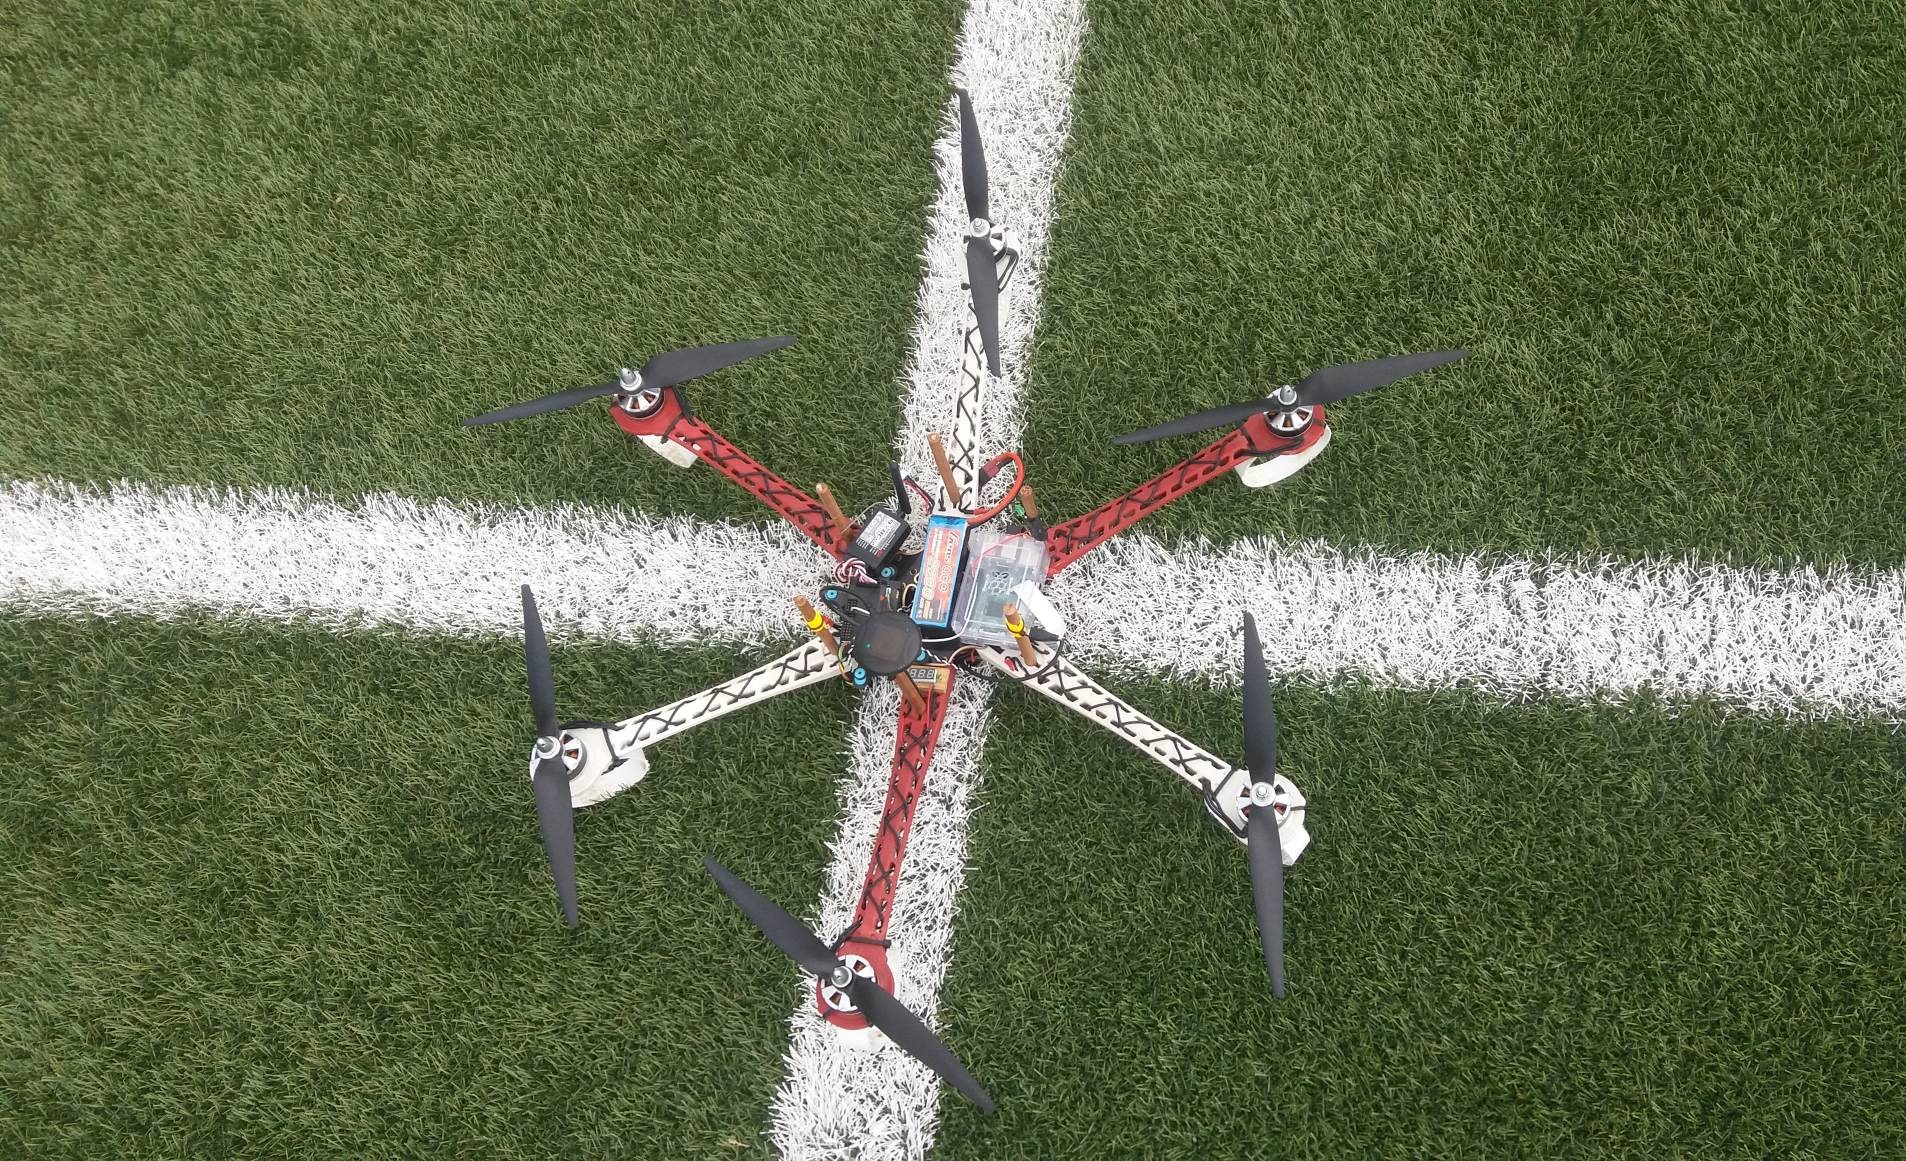
\includegraphics[scale=0.11]{images/hex3.jpg}
\caption{Hex multirotor landed}
\end{subfigure}
\begin{subfigure}{0.5\textwidth}
\centering
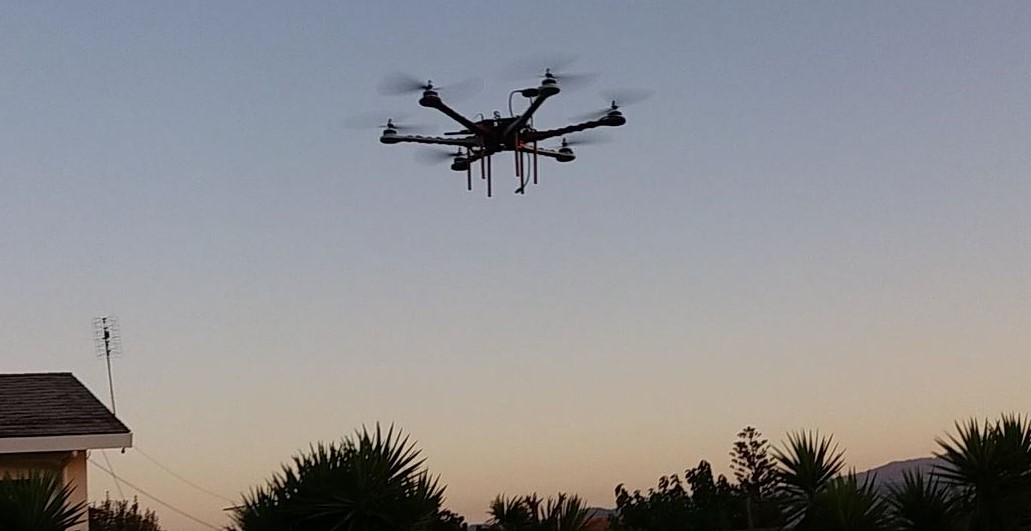
\includegraphics[scale=0.3]{images/hex2.jpg}
\caption{Hex multirotor in-flight}
\end{subfigure}
\caption{Large cinematography multirotor}
\label{fig:hex}
\end{figure}

Recreational usage may use 'mini multicopter frames' for flying indoors and outdoors \cite{frame} as in Figure \ref{fig:small_quad}. They're extremely light, but do not have enough space or power for other peripherals\footnote{GPS, Raspberry Pis etcetra}.\\

\begin{figure}[H]
\centering
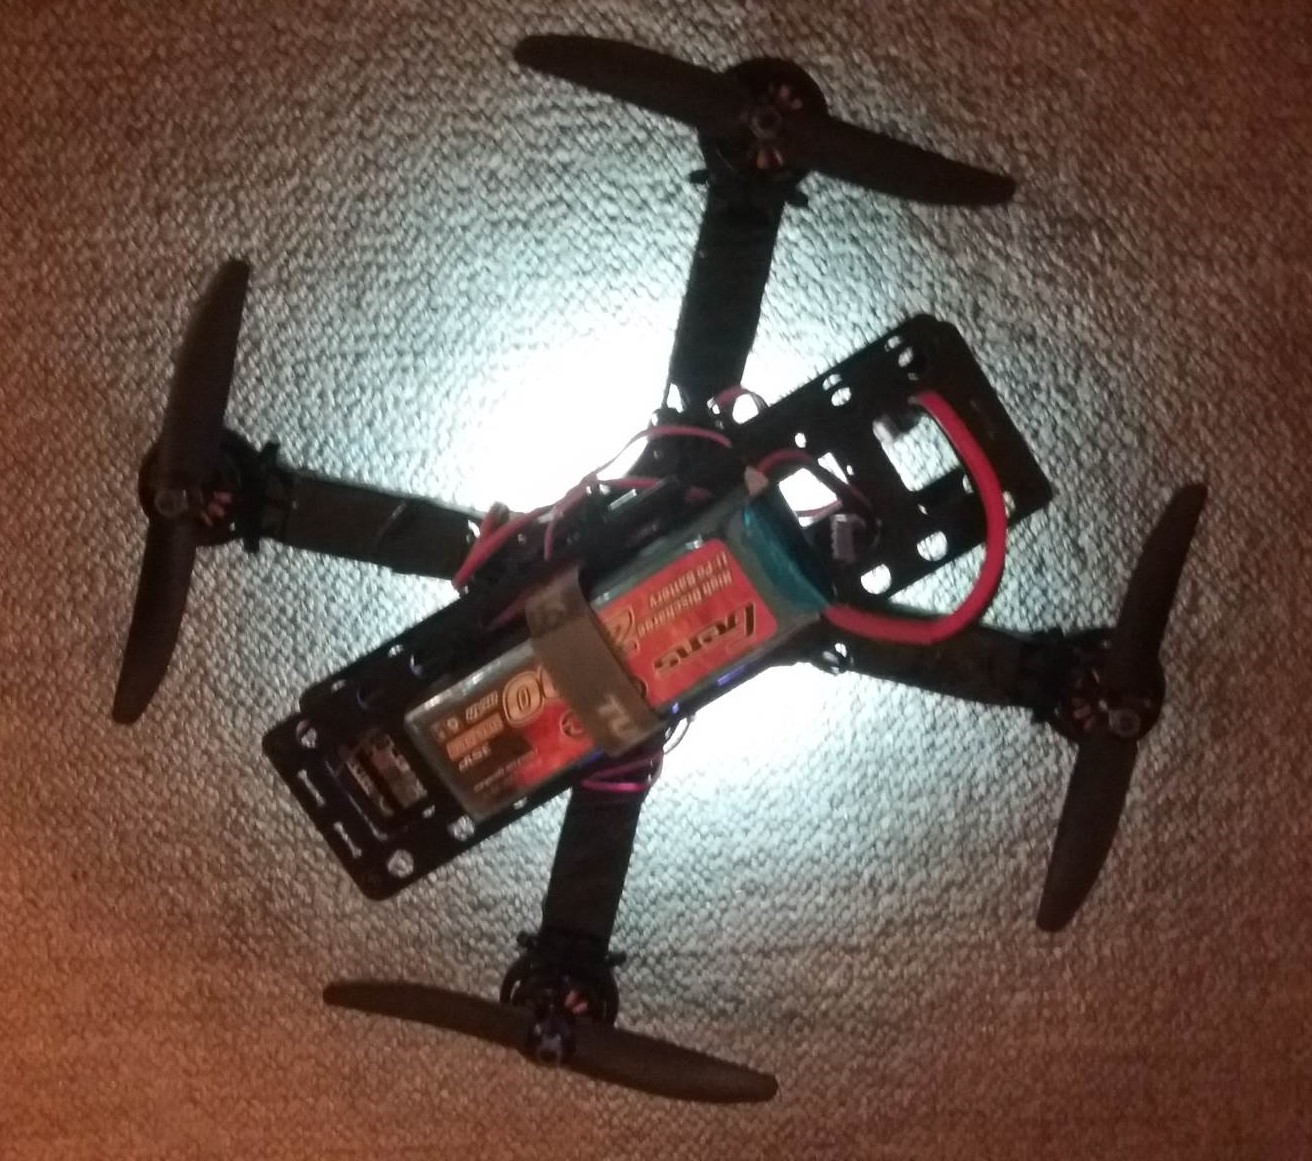
\includegraphics[scale=0.12]{images/small_quad.jpg}
\caption{Small recreational quadcopter}
\label{fig:small_quad}
\end{figure}

Sports drones are light and fast, but they require high discharge batteries. Like the quadcopter\footnote{Four propellers. Hex is 6, and `multirotors' have any number more than 2.} in Figure \ref{fig:small_quad} which has 2300 KV\footnote{KV is not kilo-volts. It is a measure of the revolutions per minute when 1 Volt is applied with no load attached to the motor} rated motors, sports/racing drones also have 2000+ KV ratings, but they will typically have thicker windings, which means it is capable of a higher wattage. One may be able to make enough room, but the batteries will not last very long.\\

A combination of these configurations means that a medium sized quadcopter/drone will be suitable. It is not too light or too heavy, and has room and power for other peripherals.\\

Materials include carbon-fibre, aluminium, fibreglass and synthetic polymers. The differences between them are not major, except that aluminium is heavier, requires larger motors and induces more vibrations. Carbon-fibre contributes to radio interference\cite{frame}, but is the lightest.\\

The closest local-supplier competition before the F450-V2 quadcopter frame was chosen was the ZMR250 Carbon Mini Quad FPV Frame as in Figure \ref{fig:zmr}.

\begin{figure}[H]
\centering
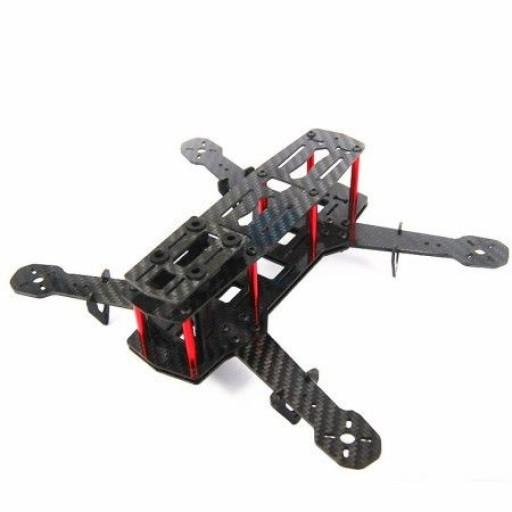
\includegraphics[scale=0.35]{images/zmr250.jpeg}
\caption{ZMR250 Carbon Mini Quad FPV Frame \cite{frobot}}
\label{fig:zmr}
\end{figure}

Both frames have roughly the same price\footnote{500 ZAR}. The ZMR250 has a carbon fibre body making it extremely light (145g), but fell into the class of `mini multicopter' as mentioned earlier. Therefore due to its local availability and accommodating space, the F450-V2 frame was chosen as in Figure \ref{fig:frame}.

\subsubsection{Landing Gear}

Four lengths of 10mm pine dowels approximately 15mm long were used. They totalled about 10 ZAR. The frame has 5cm legs, but accomodation has to be made for the nadir cameras.

\subsubsection{Motors}

The motors are rated at 920 KV and 230 W. This is relatively low compared to the more common racing motors with around 2000 KV or more (which the ZMR250 frame would use). KV is related to the power output and torque level of a motor. This is determined by the number of turns on the armature and the strength of the magnets.\\

\begin{figure}[H]
\centering
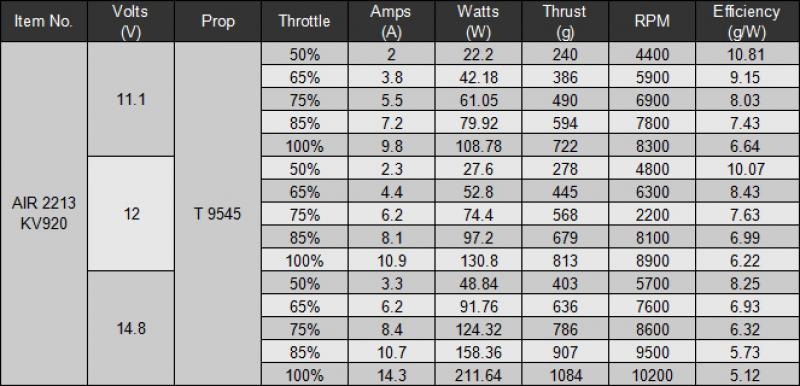
\includegraphics[scale=0.4]{images/motor_specs.jpg}
\caption{Motor and propeller combination specifications \cite{frobot}}
\label{fig:mot_prop_specs}
\end{figure}

Besides the many other characteristics, at maximum throttle, and using 3 cell batteries, the thrust is determined to be 3252 g in Figure \ref{fig:mot_prop_specs}. This gives a thrust to weight ratio of 2.95, which is satisfactory.

\subsubsection{Propellers}

The propellers have a pitch of 4.5', which is basically a measure of the 'bite', or distance it travels through the air on one revolution.

\subsubsection{Protective enclosure}

A housing is needed to protect the exposed electronics from the elements. Also, dramatic airflow can affect the barometer readings. A case \cite{3d_case} was 3D printed for the Navio2 and Raspberry Pi as in Figure \ref{fig:fcarpc2}.

\begin{figure}[H]
\begin{subfigure}{0.5\textwidth}
\centering
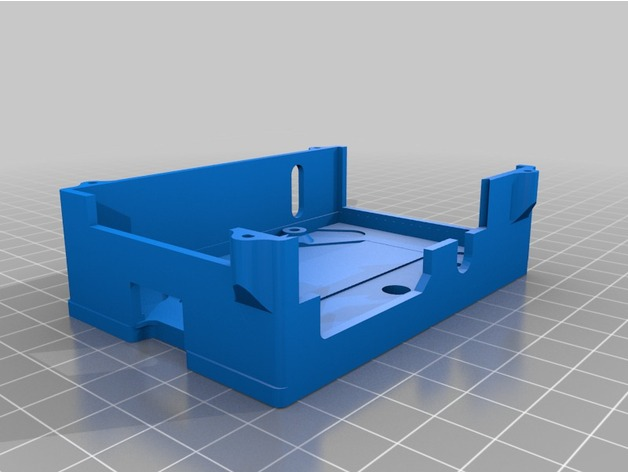
\includegraphics[scale=0.25]{images/drone-build-3d-case-render.jpg}
\caption{Case render}
\label{fig:fcarpc1}
\end{subfigure}
\begin{subfigure}{0.5\textwidth}
\centering
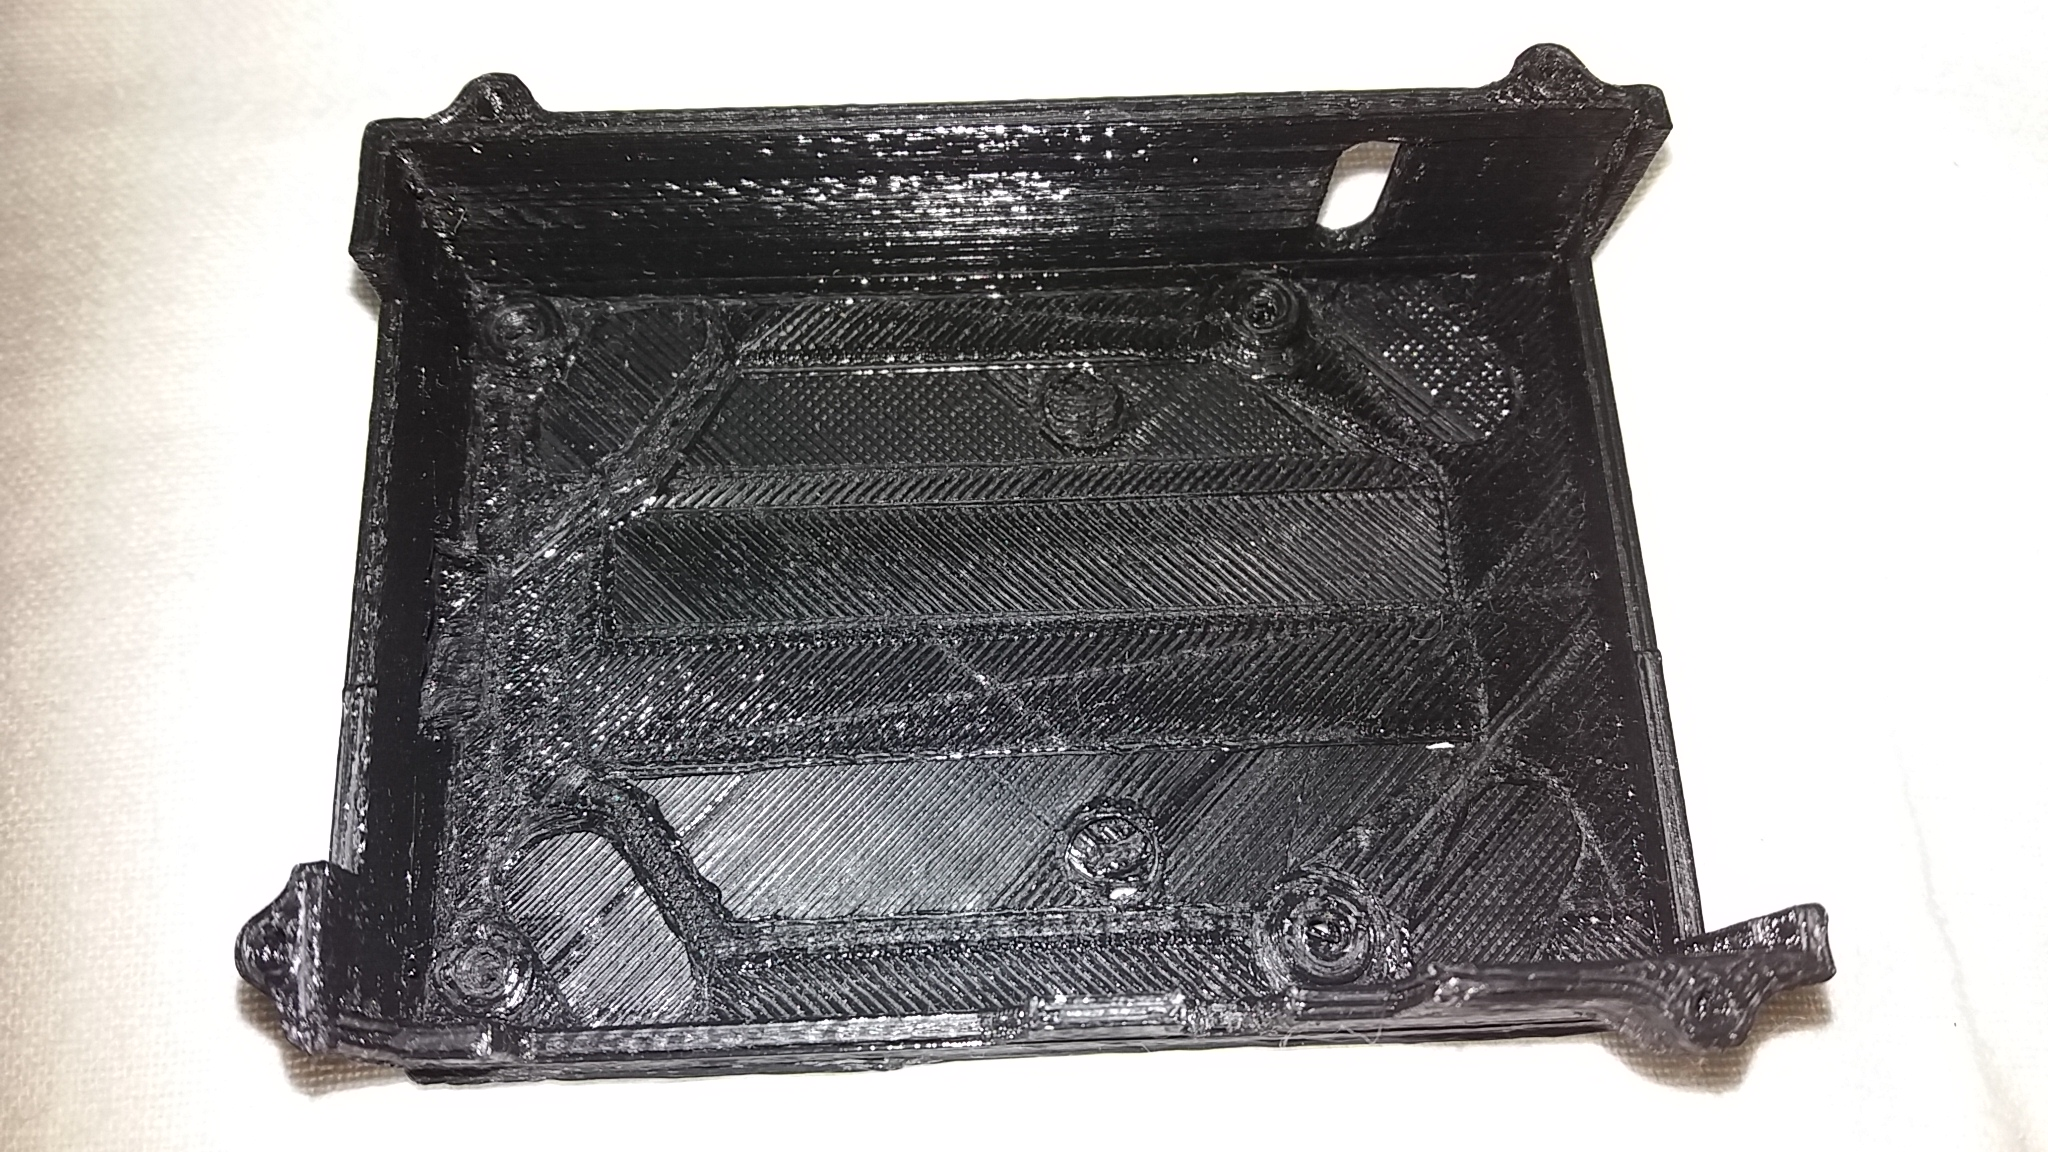
\includegraphics[scale=0.1]{images/drone-build-3dcase.jpg}
\caption{3D printed case for Raspberry Pi and Navio2.}
\label{fig:fcarpc2}
\end{subfigure}
\caption{Flight controller and Raspberry Pi case}
\label{fig:fcarpc}
\end{figure}

\subsection{Electrical subsystem design}
\subsubsection{Batteries}

Multiple 3S1P batteries will be used as in Figure \ref{fig:batteries}, since the price cost-point was the cheapest from Goblin Hobbies.\\

\begin{figure}[H]
\centering
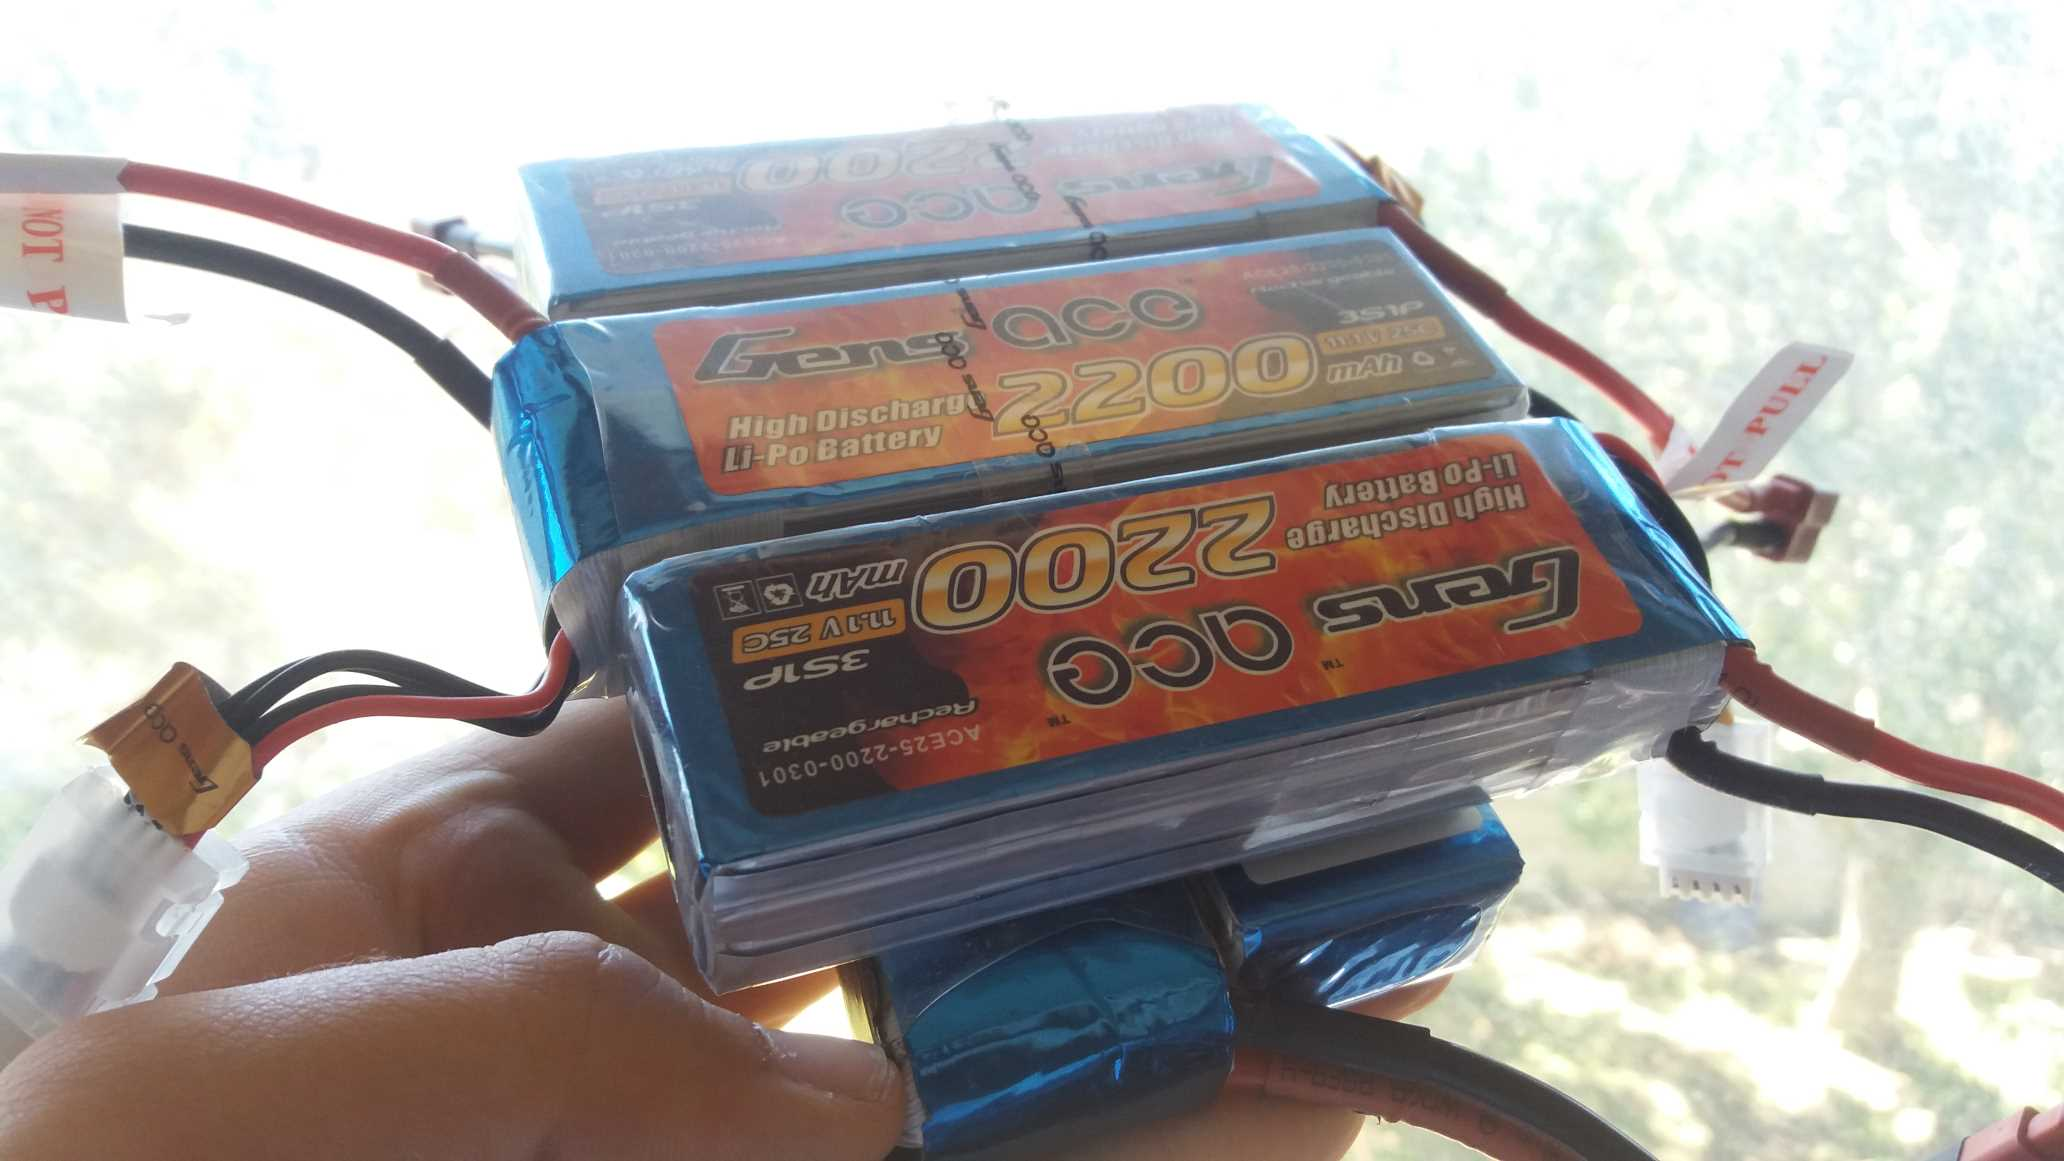
\includegraphics[scale=0.17]{images/batteries.jpg}
\caption{3SP1 GensAce Lithium batteries}
\label{fig:batteries}
\end{figure}

They are charged using a balance-charger, which charges all three cells equally so that they all age the same. Otherwise cells may burst, or cause damage due to the discrepancies.\\

With an average current draw of 20 A, each battery will only last 6.6 minutes, but long missions can be interrupted easily as noted in Section \ref{sec:dual_power}.

\subsubsection{Dual power redundancy}
\label{sec:dual_power}

The flight controller takes in two power source inputs for dual redundancy as in Figure \ref{fig:dual_redundancy}. One of the batteries powers the motors during flight. This also allows the electronics to remain on when swapping out the flight battery.

\begin{figure}[H]
\centering
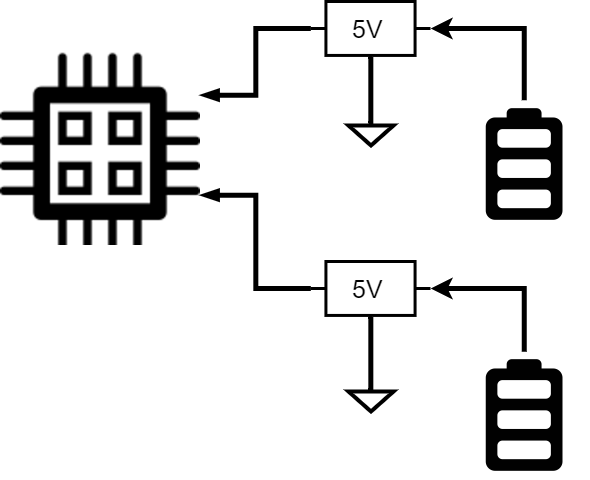
\includegraphics[scale=0.35]{images/dual_redundancy.png}
\caption{Illustrating dual power redundancy}
\label{fig:dual_redundancy}
\end{figure}

\subsubsection{Electronic speed controllers}

The 3-phase motors require speed control. This is achieved by ESCs. Maximum power draw from the motors is 18A. 20A rated ESCs are used.

\subsection{Processor subsystem design}

The Navio2 flight controller fits perfectly onto the Raspberry Pi's 40-pin header in Figure \ref{fig:insertion_navio}. It also uses every signal pin, except for one. The Navio2 communicates directly with the Broadcom CPU on the Pi, resulting in a multi-processor system. The greatest significance in this case is that flight variables can be monitored and controlled. It is non-trivial in standalone flight controllers, as the on-board firmware has to be modified with utmost care.\\

The Navio2 has a co-processor to handle PPM/Sbus inputs and provides PWM output for the ESCs.

\subsection{Control subsystem design}

\subsubsection{Flight controller}
Flight controller is needed to stabilize the airborne vehicle, and set mission waypoints. The Raspberry Pi, Navio2, and camera symbiosis was good since all three together are quite configurable even during flight, compared to other solutions which require hands-on intervention.\\

The Navio2 was chosen specifically for its harmonious relationship with the Raspberry Pi.

\subsubsection{Flight modes}

Loiter mode uses GPS to maintain altitude and location. Altitude hold only uses the barometer. Stabilize mode gives the pilot full control of the throttle, and can be used to quickly change height, albeit it is a bit dangerous. Auto mode is used to fly autonomously in missions. Return to launch (RTL) uses GPS and does as its namesake suggests. Brake mode is used to pause its current activity, and if moving quickly it will actively brake by tilting in the other direction to prevent drift. All these flight modes can be accessed in flight by the remote controller, except Auto mode which is activated using the GCS.

\subsection{Communication subsystem design}
\label{sec:comms}

The drone communicates with the handheld remote controller via S-BUS, which is a universal standard. The beauty of it is that it communicates with one signal wire as in Figure \ref{fig:attach_sbus}. Previous implementations one may have had to use pulse position modulation (PPM), where each channel requires a wire. Even though this may sound simple, it does increase PCB size, complexity and cost in the end. One the same note, each electronic speed controller (ESC) gets a signal wire and power input.

%(add picture showing all the wireless technologies)\\

The drone can communicate via wifi as its medium of wireless telemetry; but the interference from other devices in the crowded 2.4 GHz ISM band drastically reduces range -- especially from the handheld remote controller. That, and the wifi dongles that were available seemed to work only for about 10 m.\\

Thus, 433 MHz 100mW transceivers were connected between the GCS and the drone as in Figure \ref{fig:attach_433}, at a 56400 baudrate. Real-time telemtery to a ground station is useful for pre-flight checks, in-flight monitoring and control, and missions.\\

For development purposes, wifi is used extensively to SSH into the Raspberry Pis and to analyse photos using SAMBA. It should be noted that due to the conflict with the remote controller, it is not possible to view photos in-flight. Nevertheless, there are many cases where the wifi disconnects, and it was required to have a script running to reconnect the wifi whenever it goes down (see code in appendix \ref{code:wifiup}).\\

The flight controller controls the ESCs via PWM signals as in Figure \ref{fig:pwm}. Likewise, the remote controller (as in Section \ref{sec:remote_controller}) also sends the PWM values of each channel, yet via SBus (a single-wire form of uart communication). SBus supports up to 18-channels.\\

\begin{figure}[H]
\centering
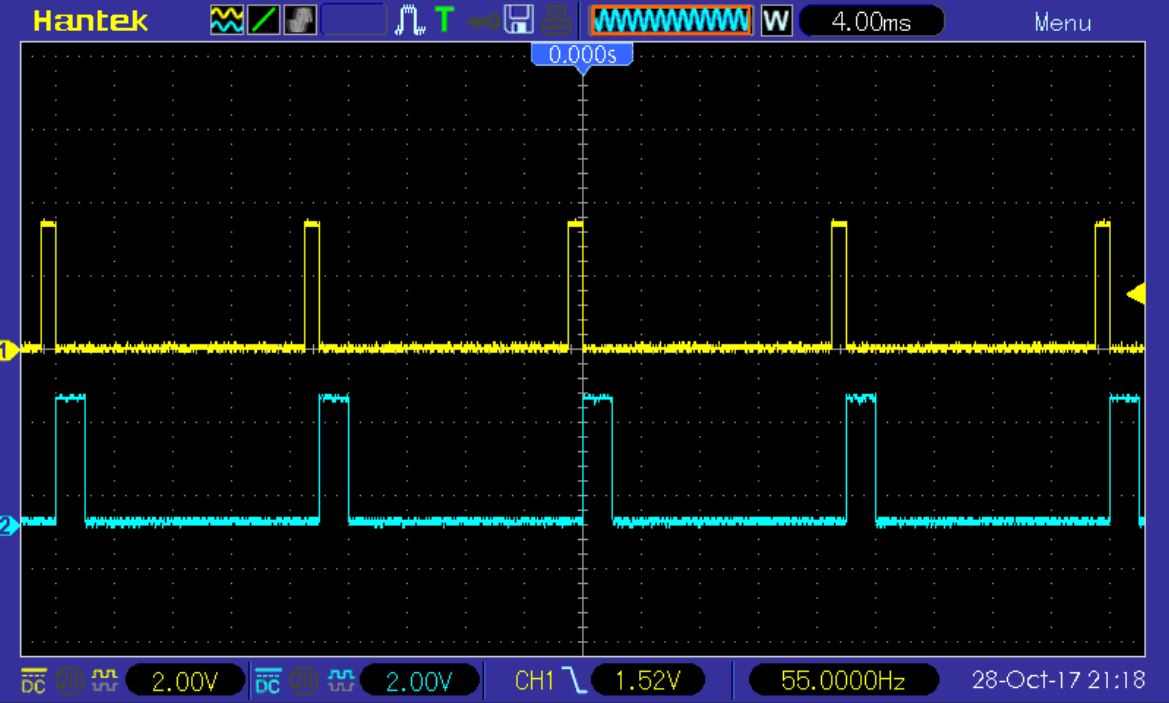
\includegraphics[scale=0.35]{images/pwm.jpg}
\caption{Min (yellow) and max (blue) duty cycle of PWM}
\label{fig:pwm}
\end{figure}

The PWM has a wavelength of 18 ms, and a duty cycle between 1 ms and 2 ms.

\subsection{Sensor subsystem design}

The flight controller has dual IMUs for redundancy, a GNSS receiver and a high resolution barometer for 10cm altitude resolution.

\begin{enumerate}
\item MPU9250 9DOF IMU
\item LSM9DS1 9DOF IMU
\item MS5611 Barometer
\item U-blox M8N Glonass/GPS/Beidou
\end{enumerate}

\subsection{Construction process and Integration}

At first, the frame is put together. This gives one a good idea of the actual size from the beginning.

\begin{figure}[H]
\begin{subfigure}{0.5\textwidth}
\centering
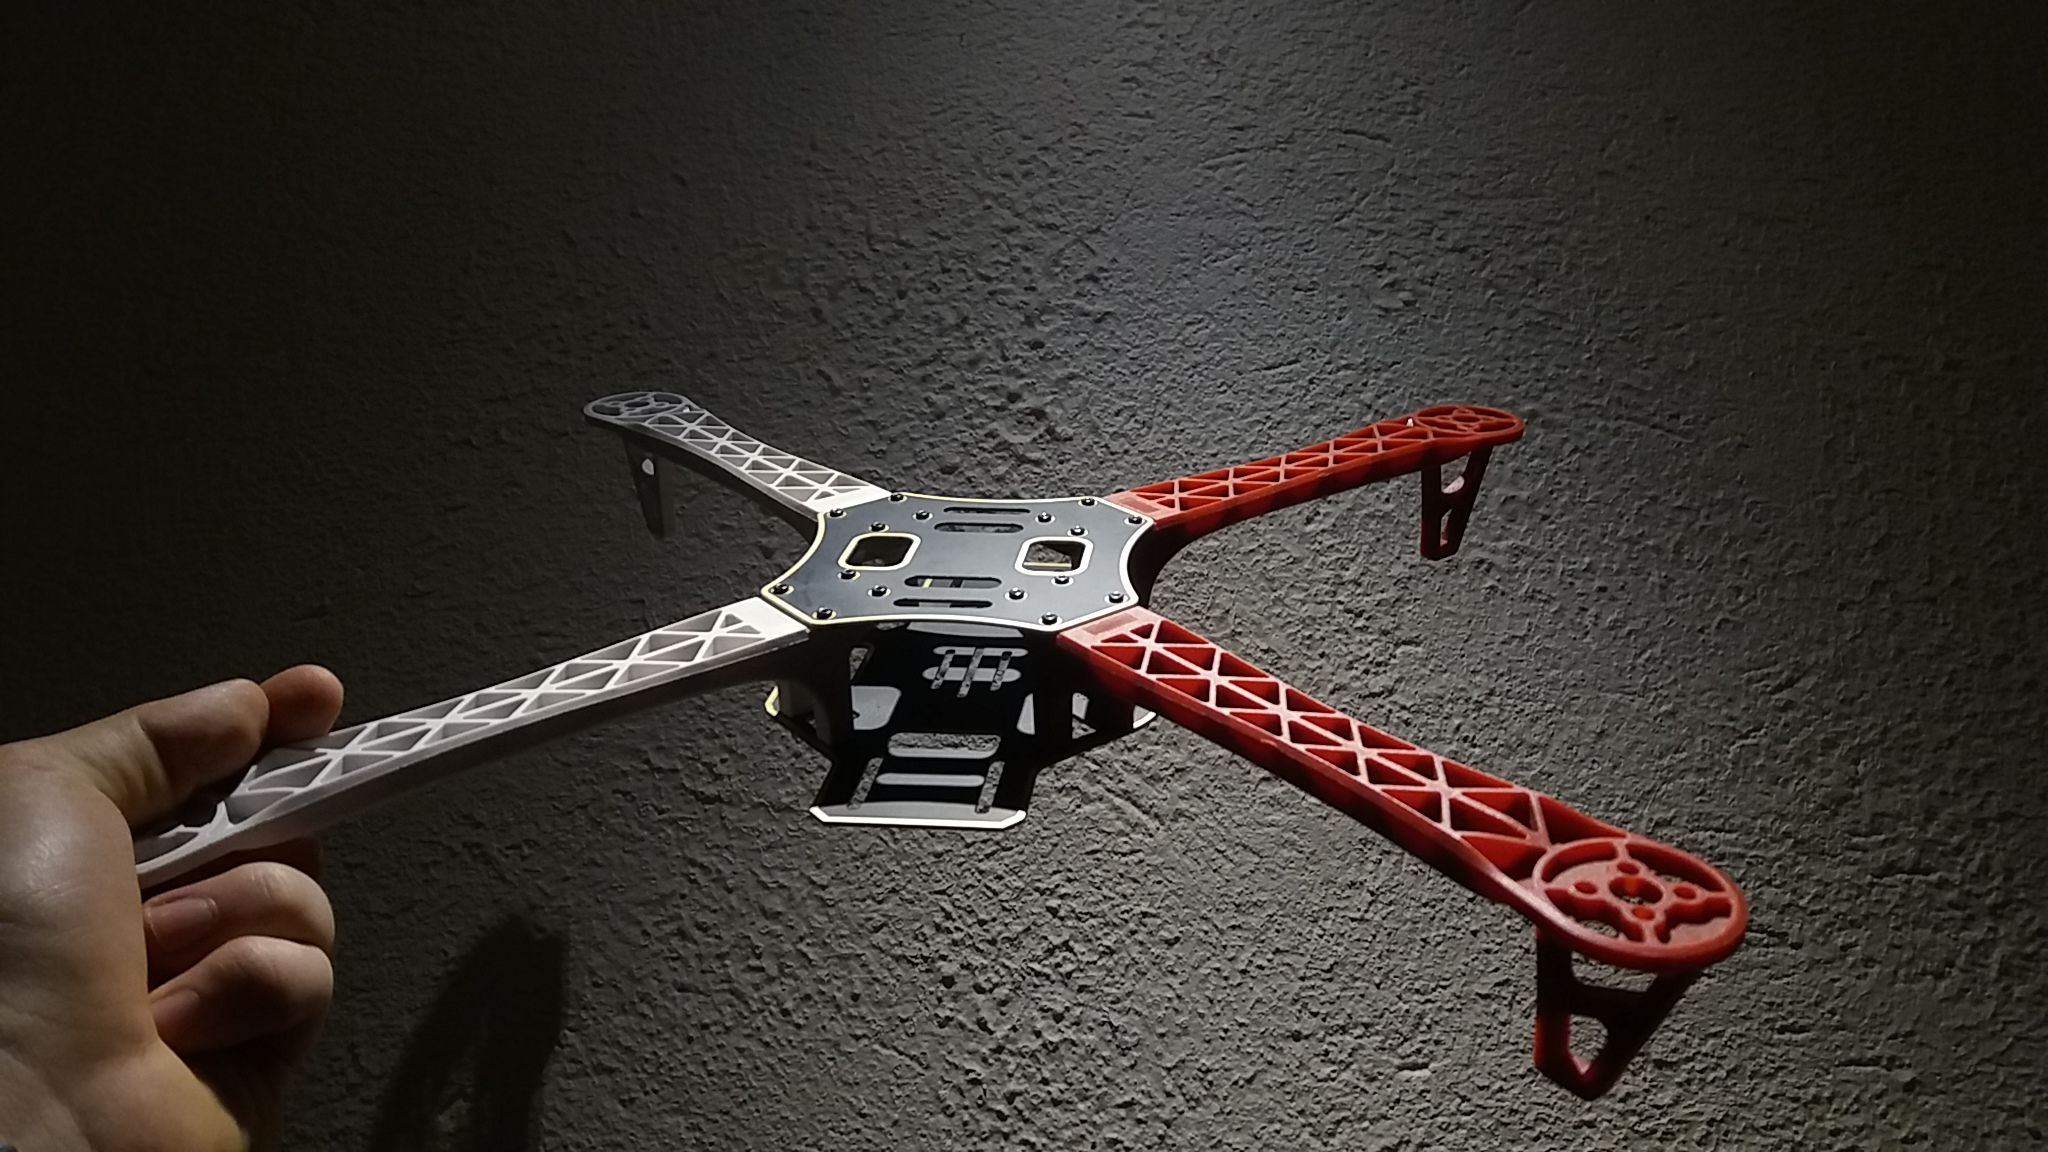
\includegraphics[scale=0.1]{images/drone-build-frame.jpg}
\caption{F450-V2 frame.}
\label{fig:frame}
\end{subfigure}
\begin{subfigure}{0.5\textwidth}
\centering
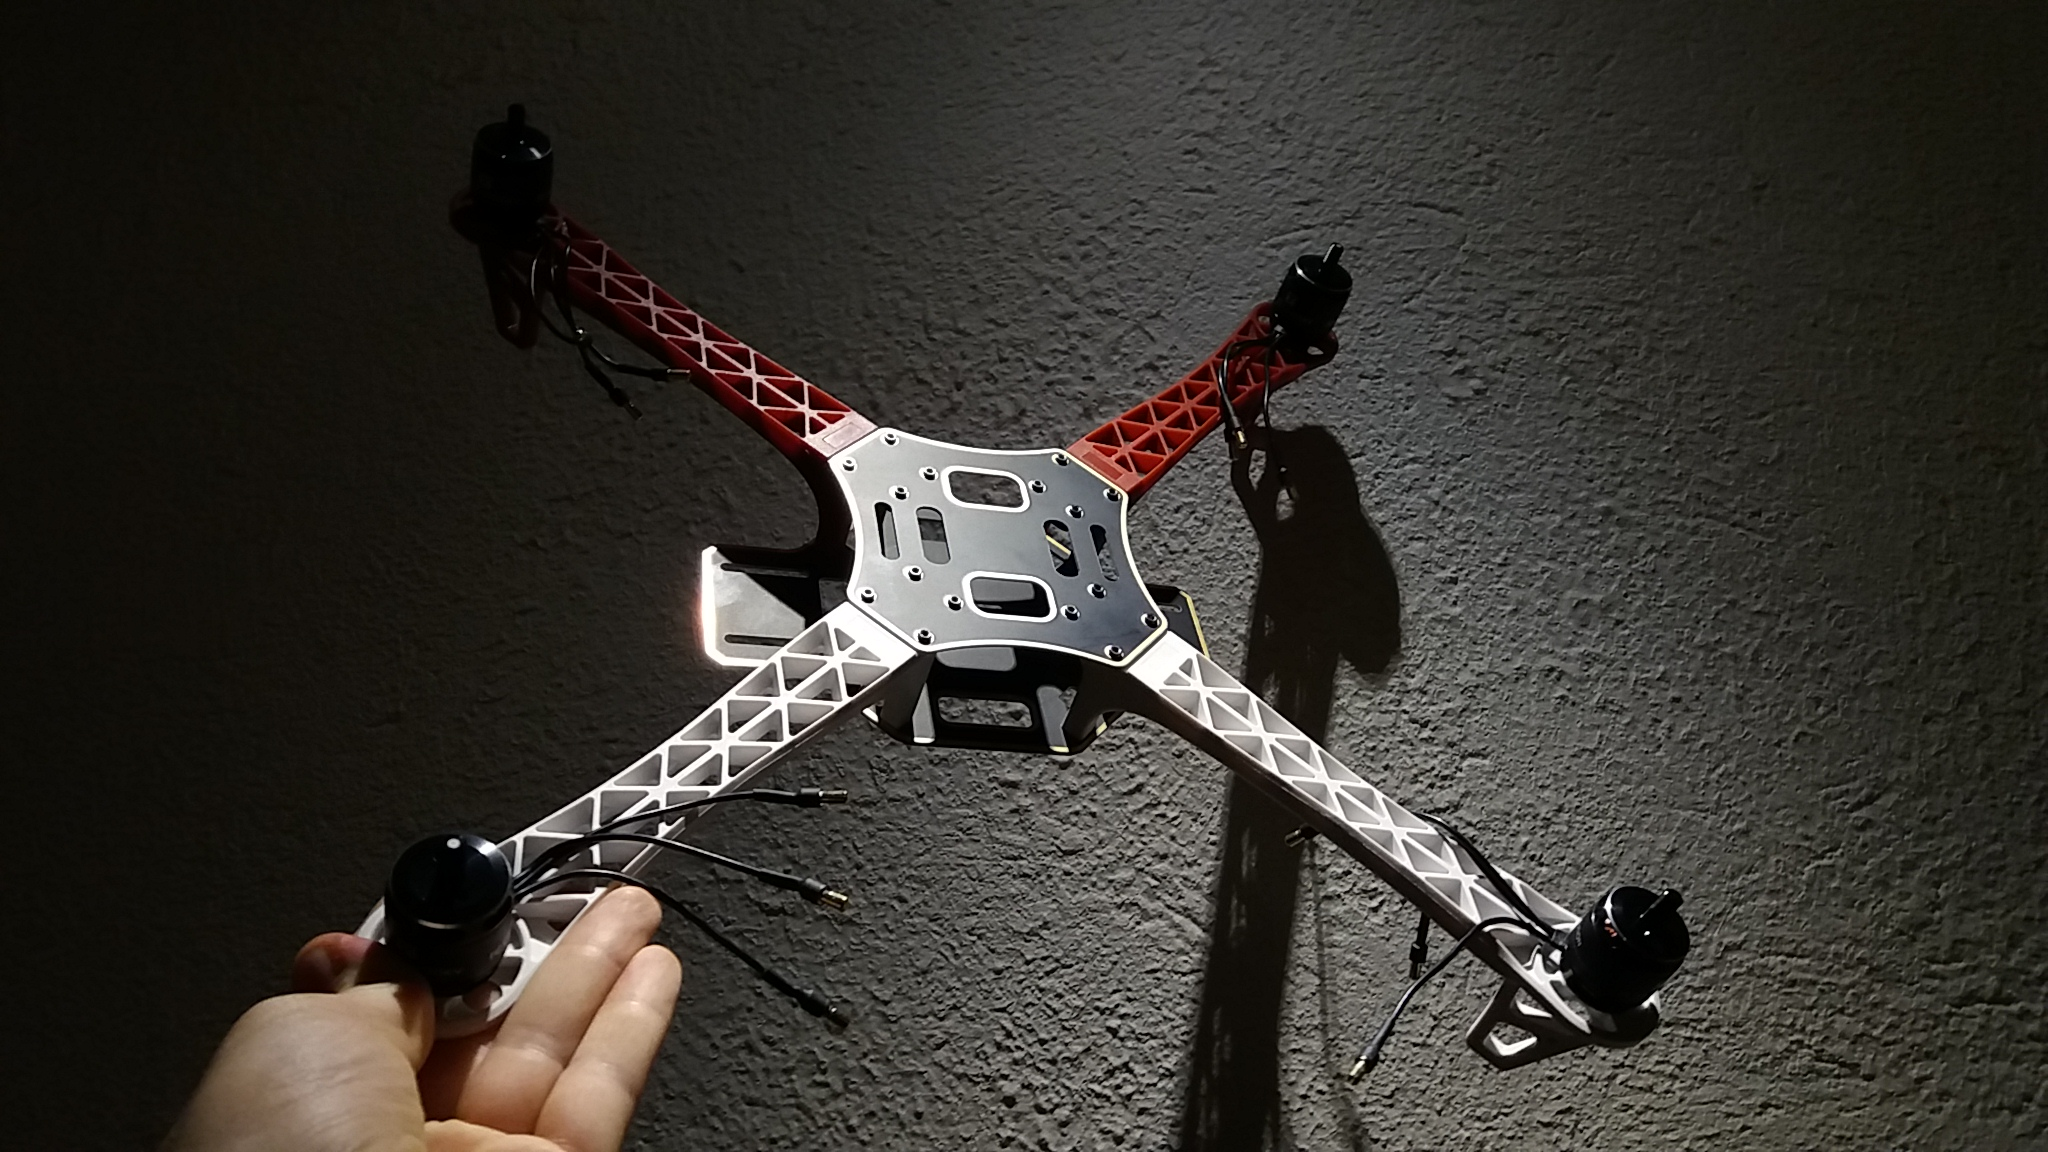
\includegraphics[scale=0.1]{images/drone-build-motors.jpg}
\caption{Adding the 920kv motors.}
\label{fig:motors}
\end{subfigure}
\caption{Frame and motors}
\label{fig:frame_motors}
\end{figure}

The nylon polymer frame as in Figure \ref{fig:frame} seems surprisingly robust, especially considering that the centre is PCB based.\\

\begin{figure}[H]
\begin{subfigure}{0.5\textwidth}
\centering
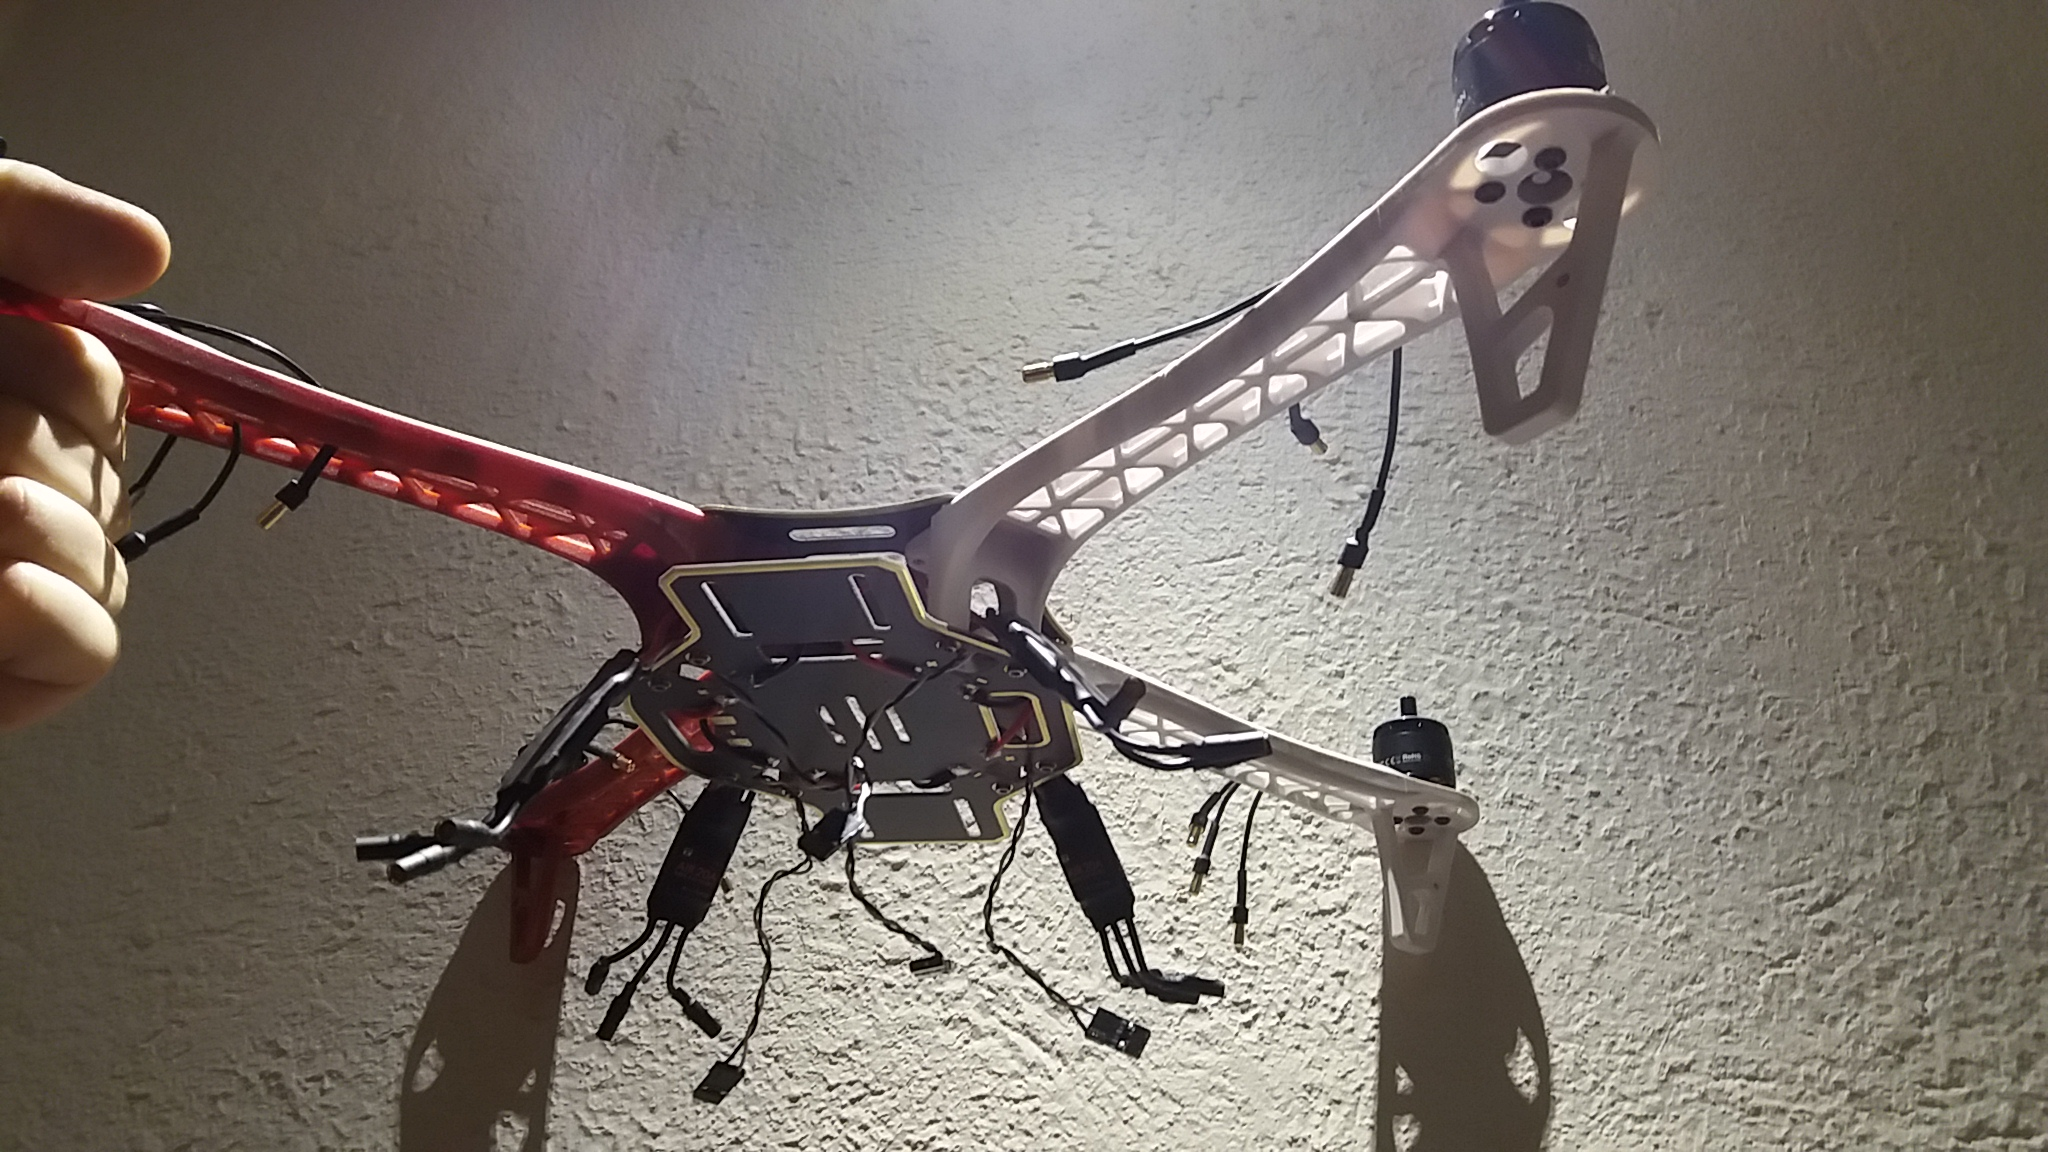
\includegraphics[scale=0.1]{images/drone-build-esc-3phaseunconnected.jpg}
\caption{Adding the ESCs. Motors require 3-phase power}
\label{fig:ESCs_uplugged}
\end{subfigure}
\begin{subfigure}{0.5\textwidth}
\centering
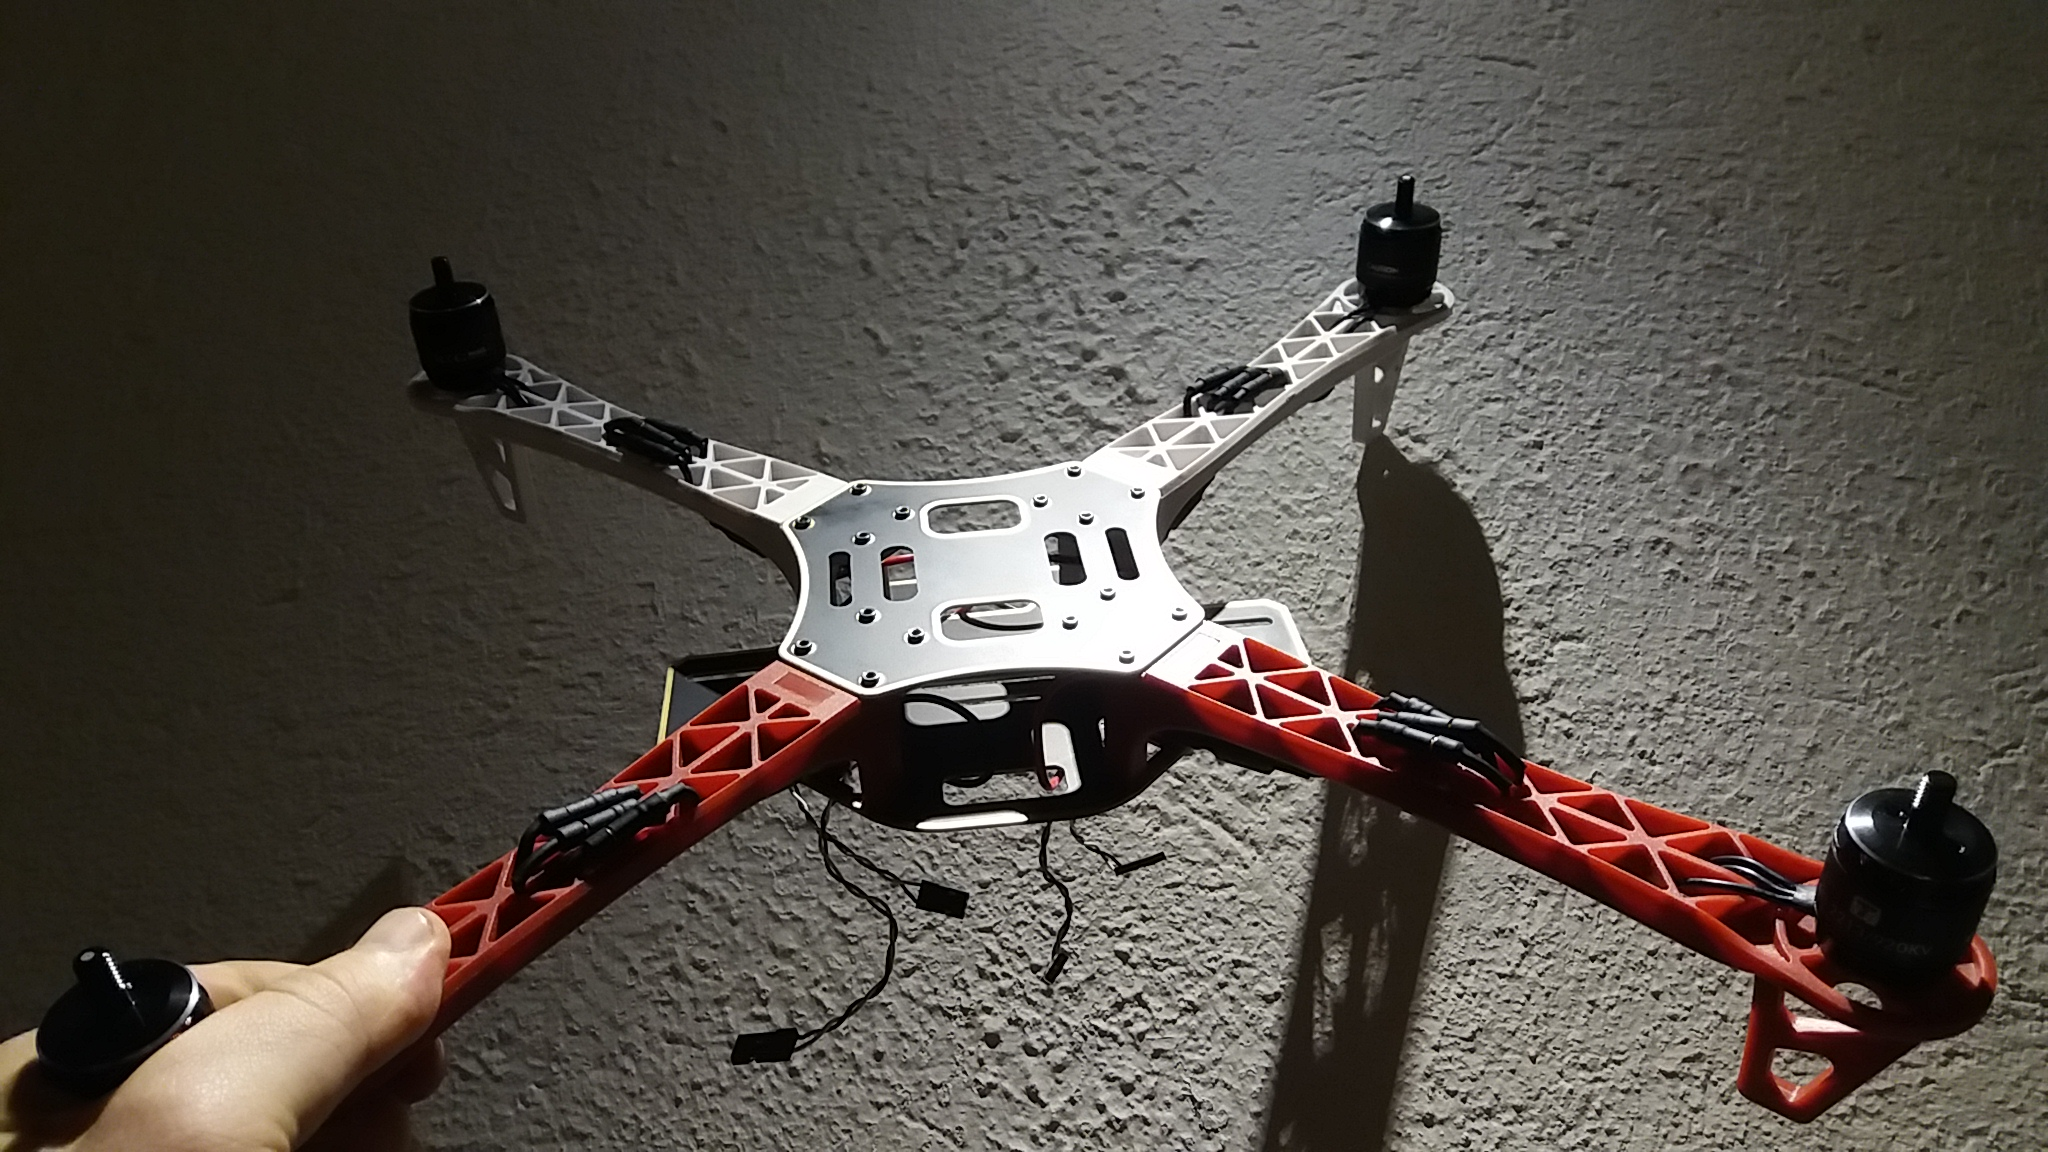
\includegraphics[scale=0.1]{images/drone-build-esc-3phaseconnected.jpg}
\caption{Power leads plugged in and secured}
\label{fig:ESCs_plugged}
\end{subfigure}
\caption{ESCs}
\label{fig:ESC}
\end{figure}

The leads are easy to plug/unplug. Any two phase leads can be swapped to change motor direction as in Figure \ref{fig:ESC}.\\

\begin{figure}[H]
\begin{subfigure}{0.5\textwidth}
\centering
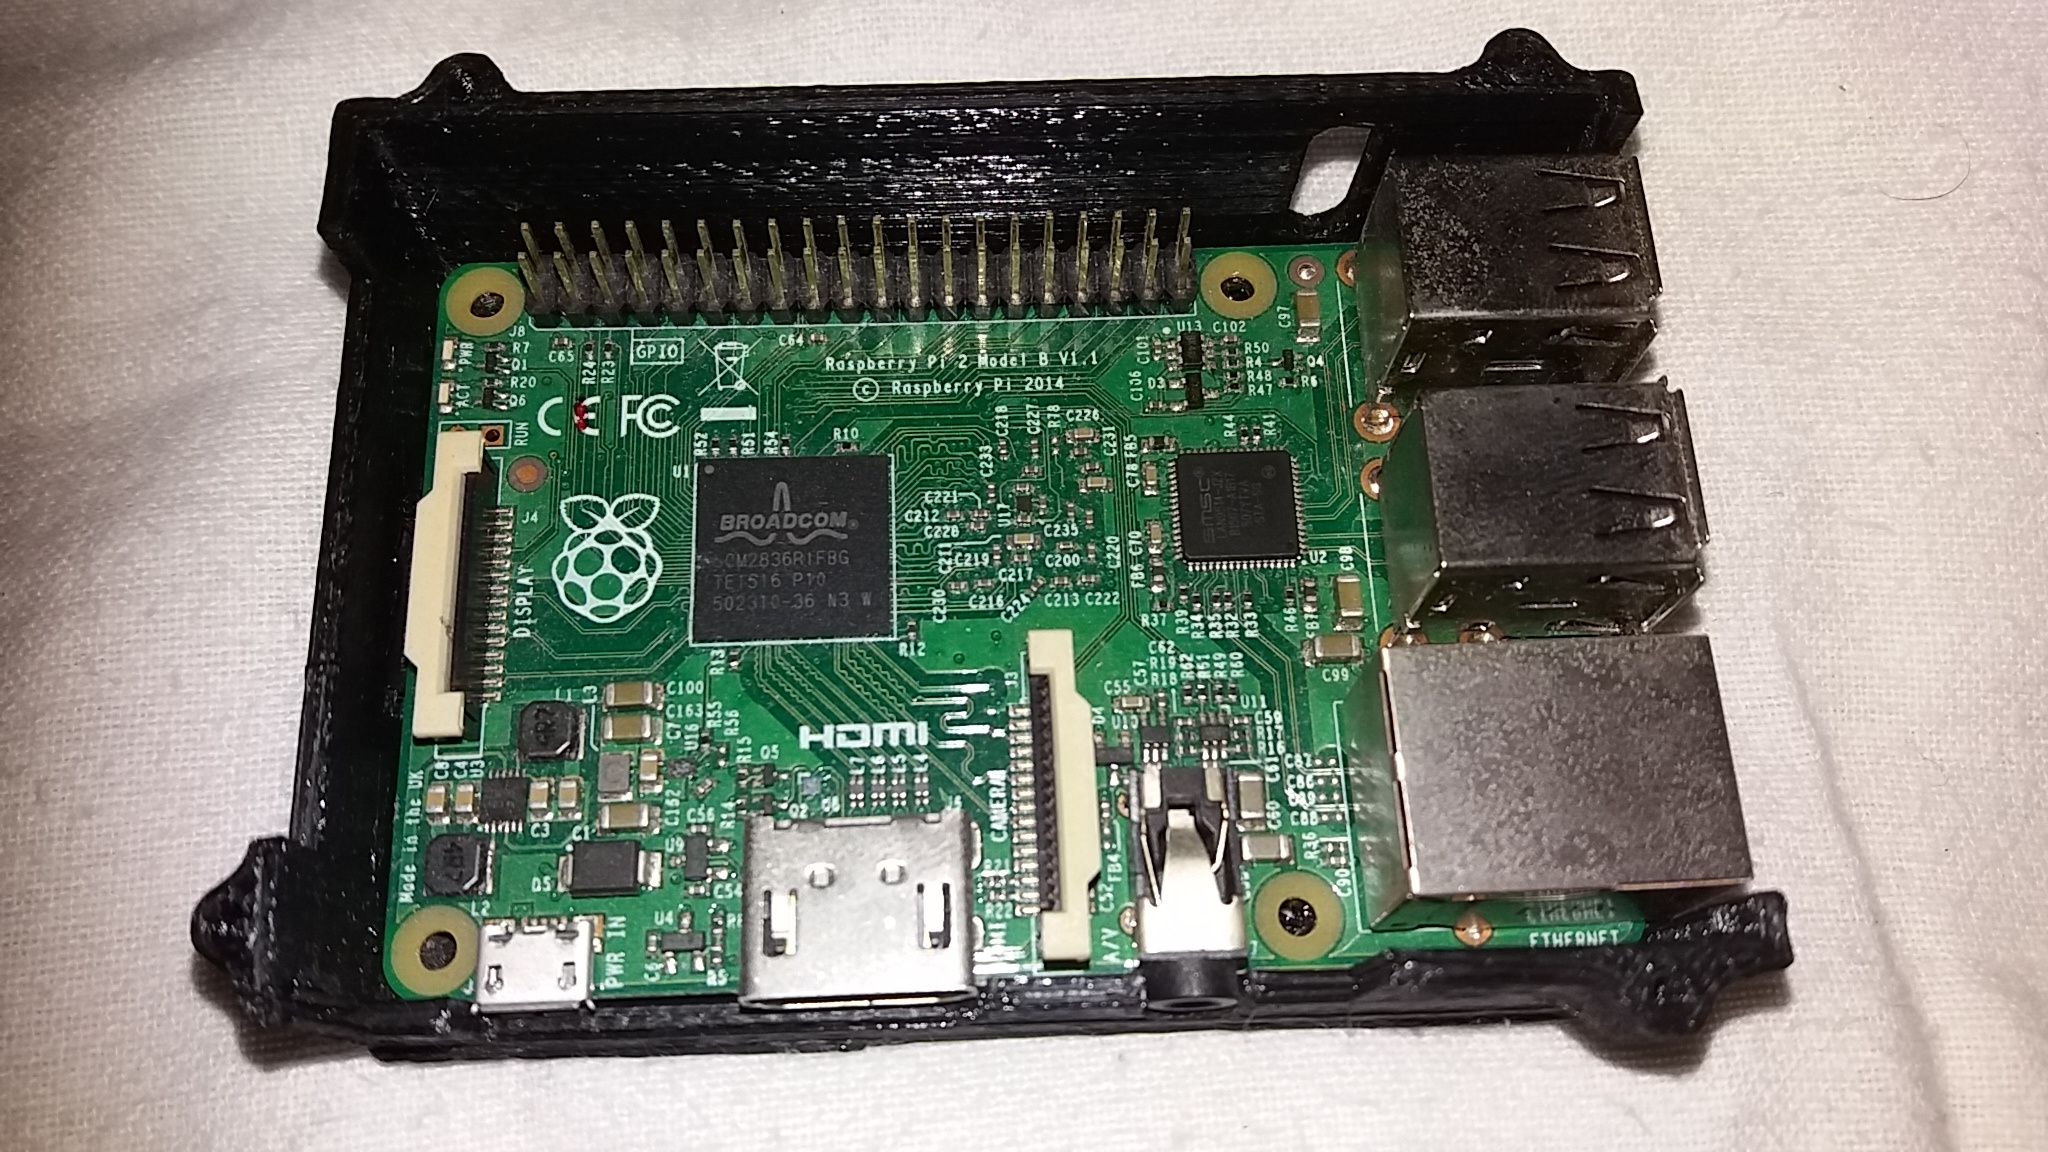
\includegraphics[scale=0.1]{images/drone-build-3dcase-pi.jpg}
\caption{Putting the Pi in the case.}
\label{fig:insertion_pi}
\end{subfigure}
\begin{subfigure}{0.5\textwidth}
\centering
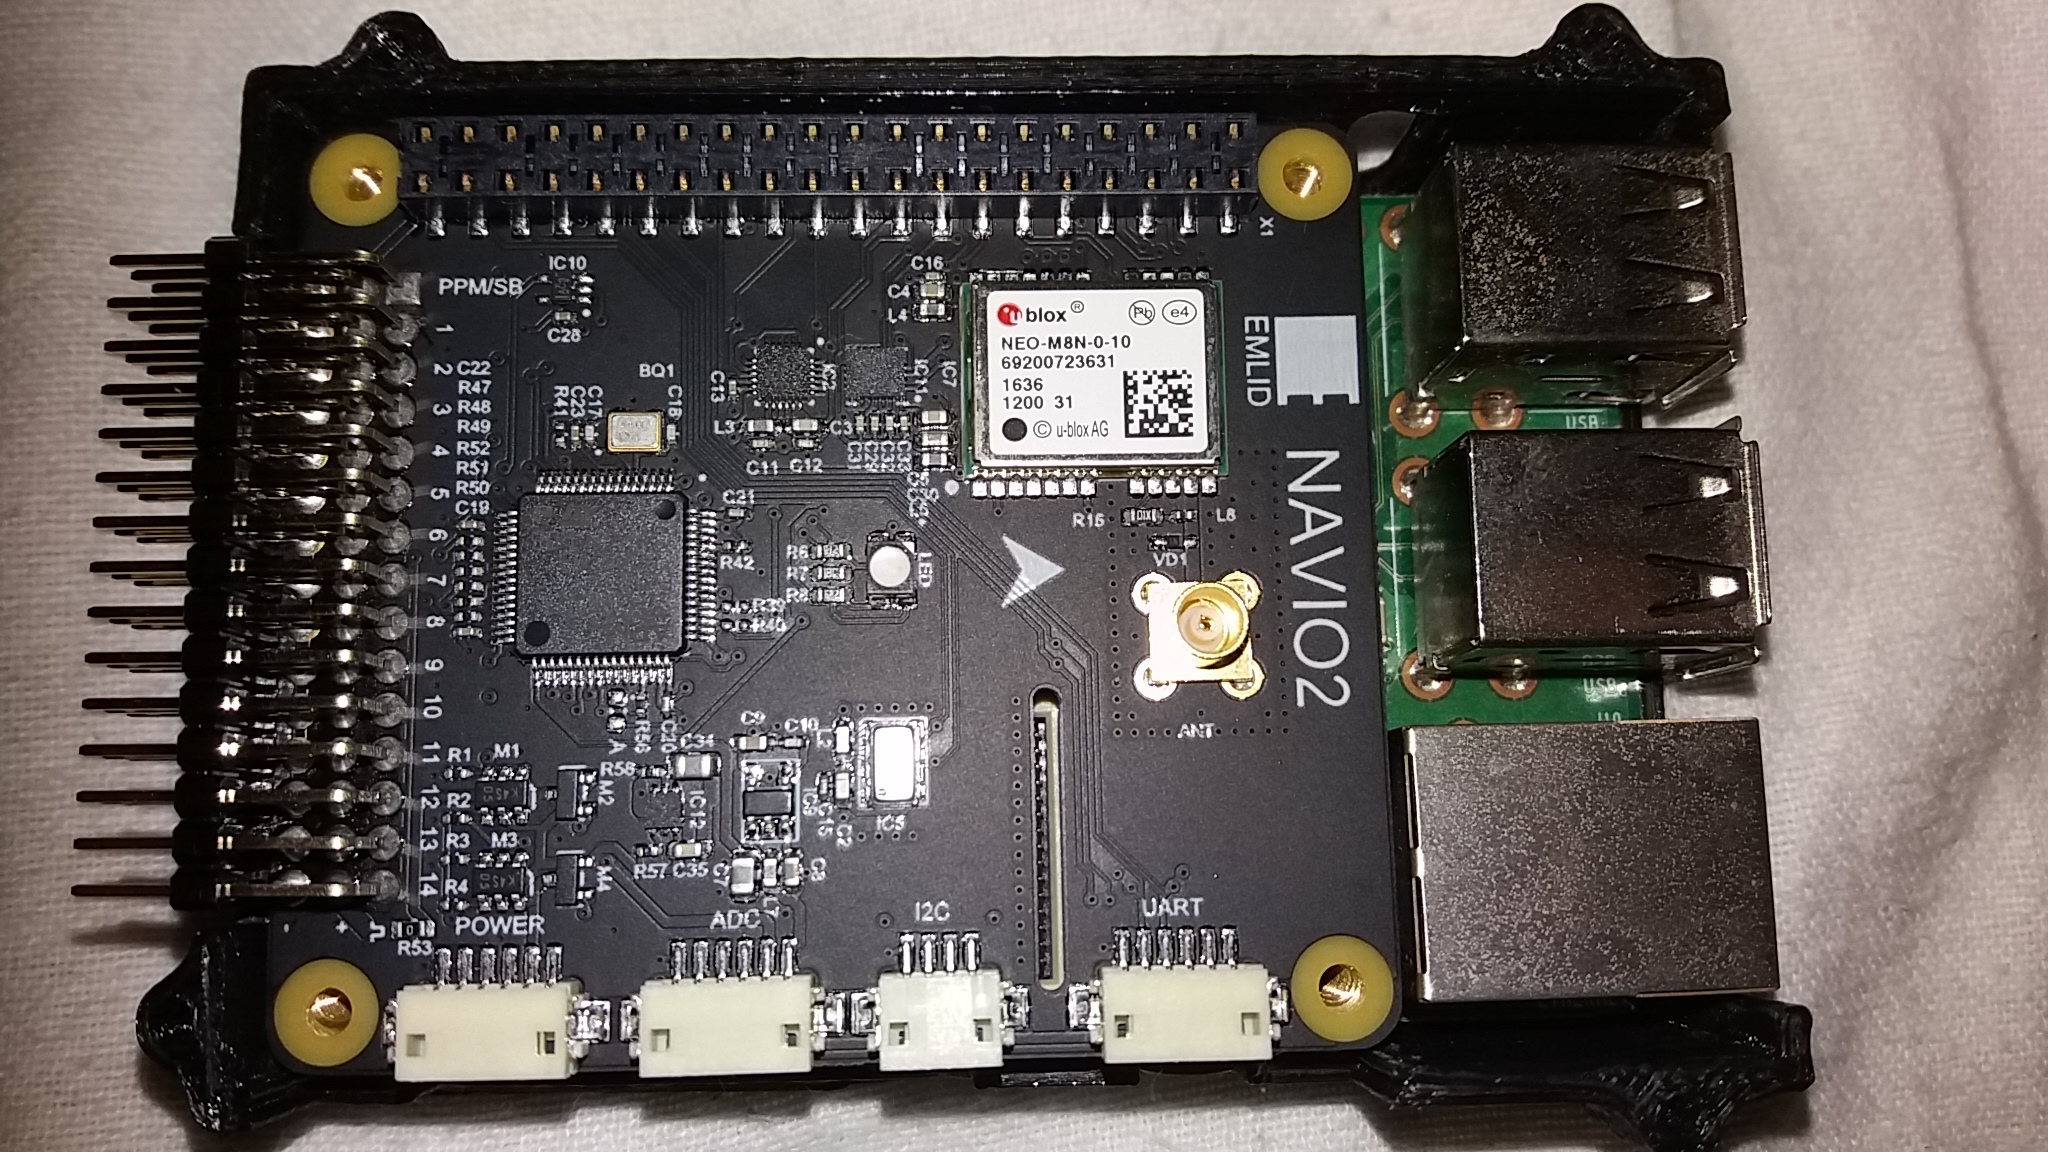
\includegraphics[scale=0.1]{images/drone-build-3dcase-pi-navio.jpg}
\caption{Fitting the Navio2 flight controller on top.}
\label{fig:insertion_navio}
\end{subfigure}
\caption{Inserting the sensitive electronics.}
\label{fig:insertion}
\end{figure}

\begin{figure}[H]
\begin{subfigure}{0.5\textwidth}
\centering
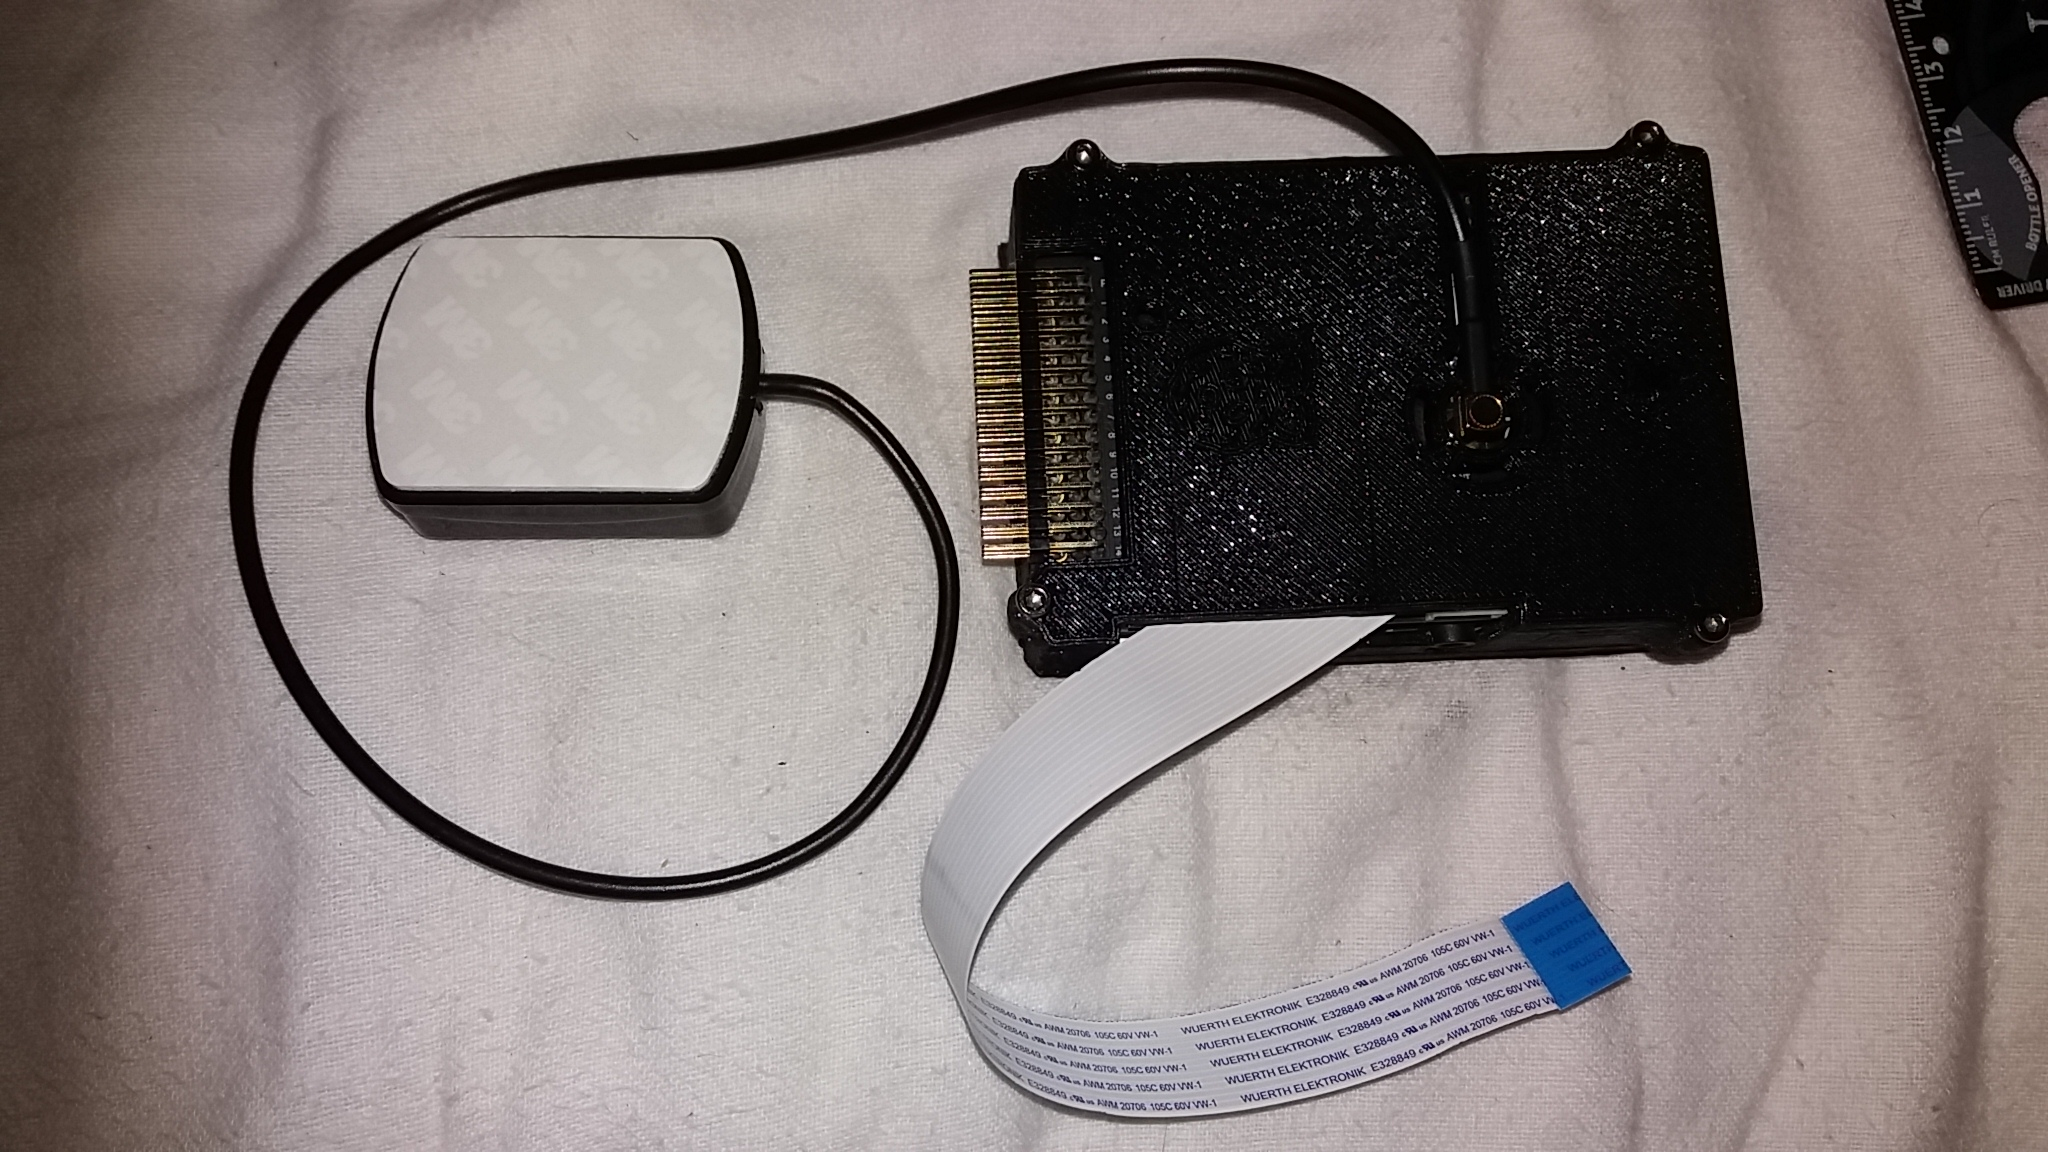
\includegraphics[scale=0.1]{images/drone-build-3dcase-gps.jpg}
\caption{Connecting Ublox Neo-7 GPS antenna and 15-pin camera CSI ribbon cable.}
\label{fig:stab_gps}
\end{subfigure}
\begin{subfigure}{0.5\textwidth}
\centering
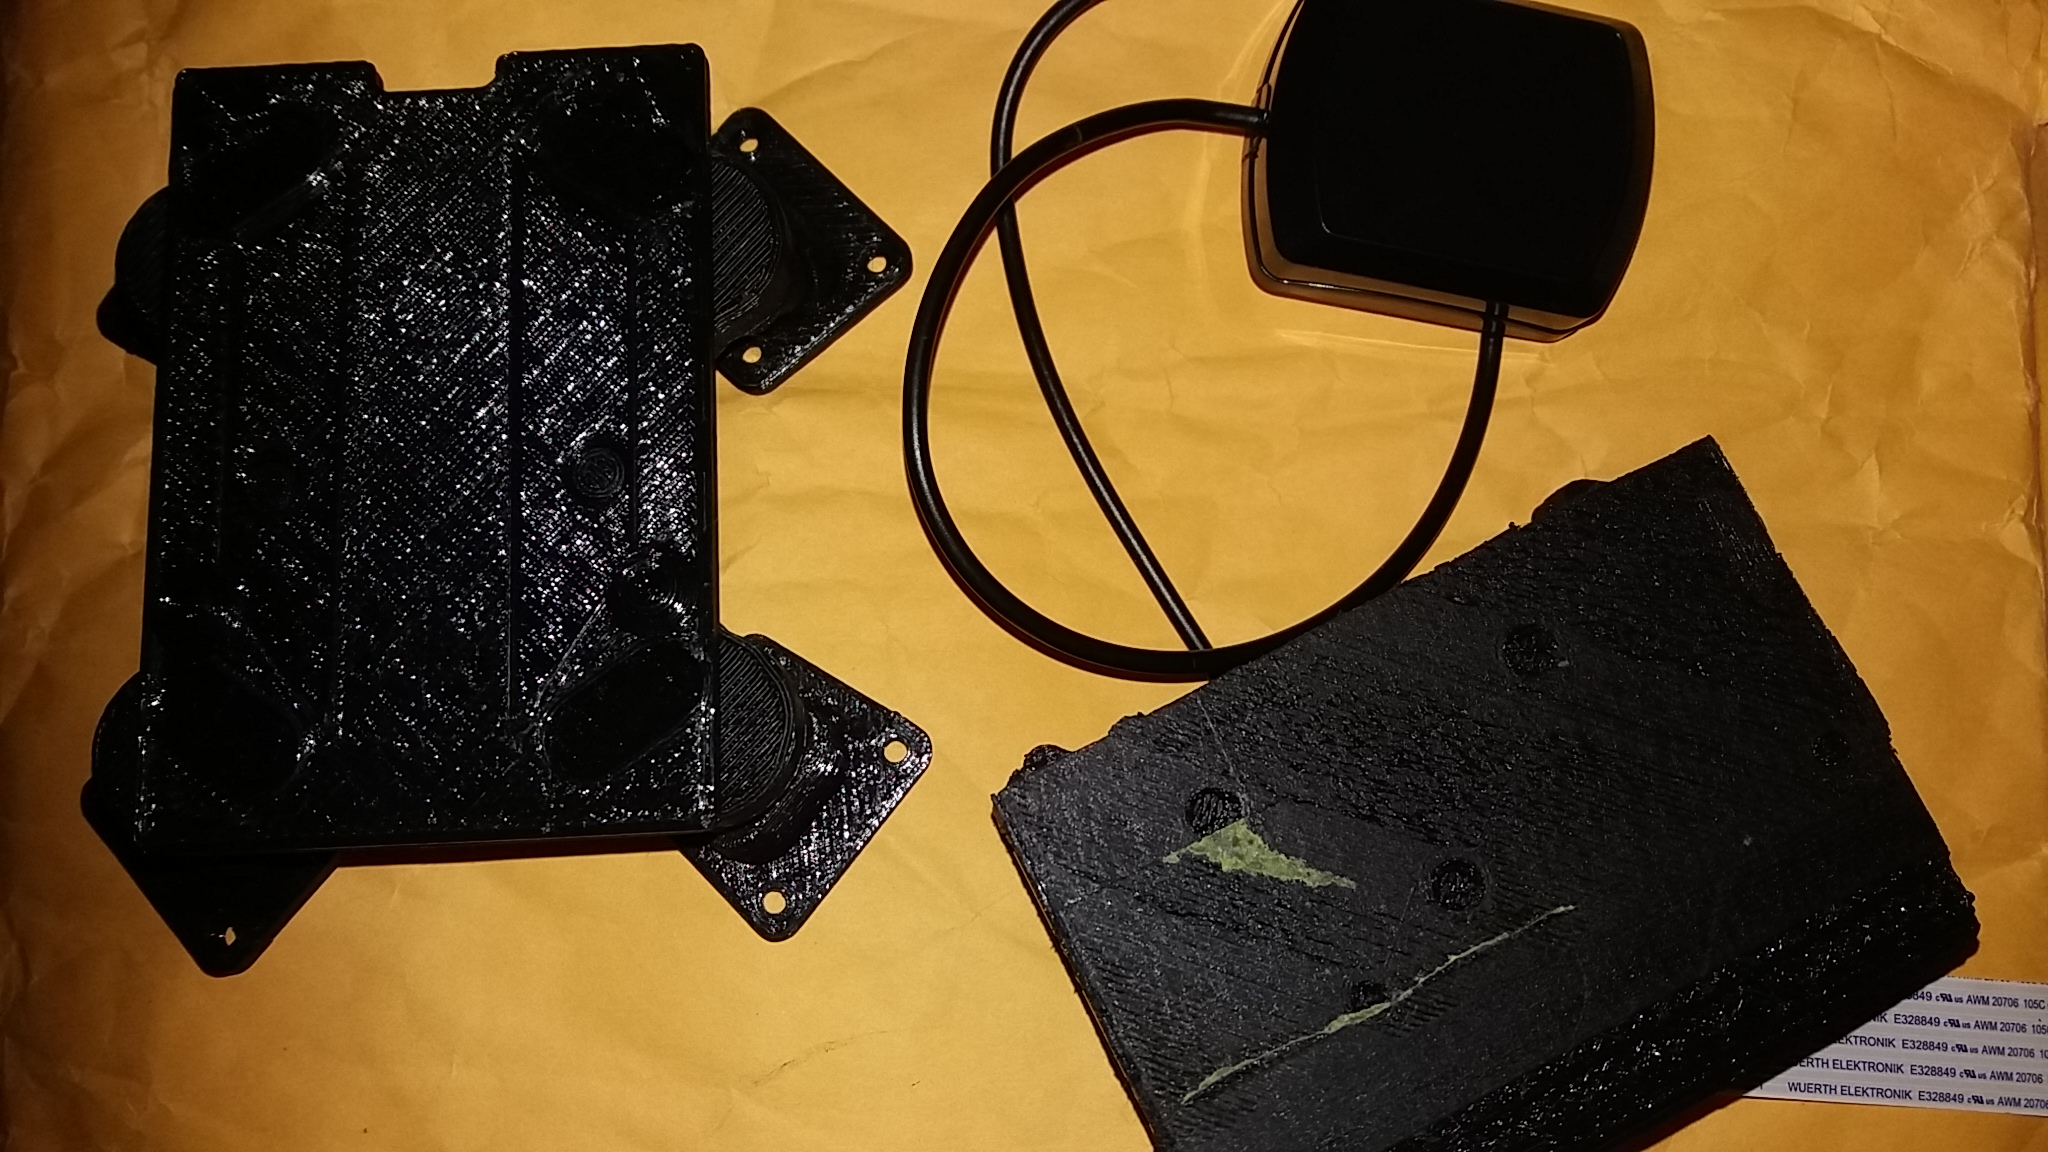
\includegraphics[scale=0.1]{images/drone-build-3dplatform.jpg}
\caption{Case and platform}
\label{fig:stab_case_plat}
\end{subfigure}
\caption{Putting the case and platform together}
\label{fig:stabilize_platform}
\end{figure}

The GPS antenna lead fits snugly onto an SMA connector in Figure \ref{fig:stab_gps}, and is exposed in such a way as to leave enough freedom for the cable to bend, but not wear as if it were rigidly attached.

\begin{figure}[H]
\begin{subfigure}{0.5\textwidth}
\centering
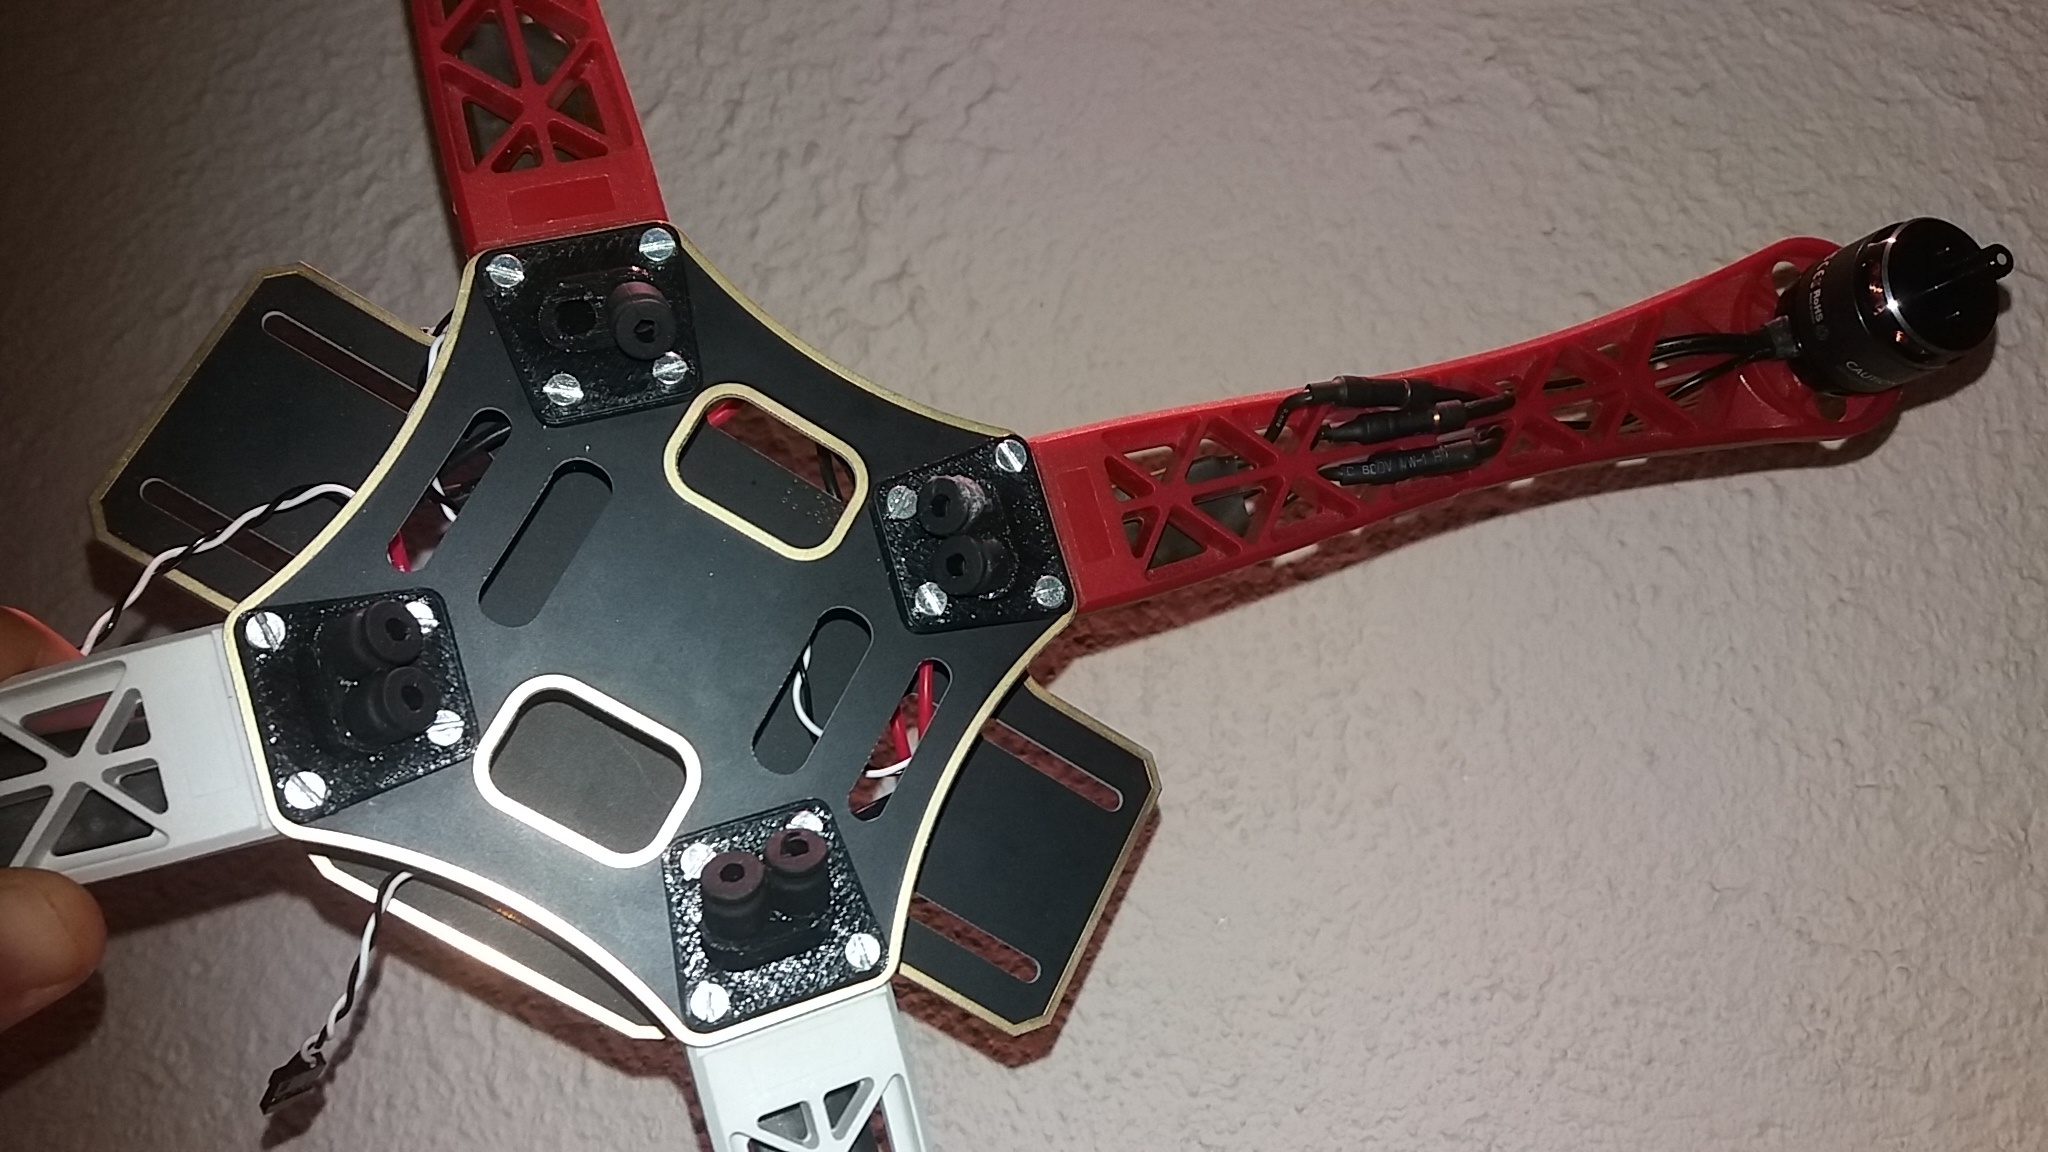
\includegraphics[scale=0.1]{images/drone-build-feet.jpg}
\caption{Added feet for platform.} 
\label{fig:feet}
\end{subfigure}
\begin{subfigure}{0.5\textwidth}
\centering
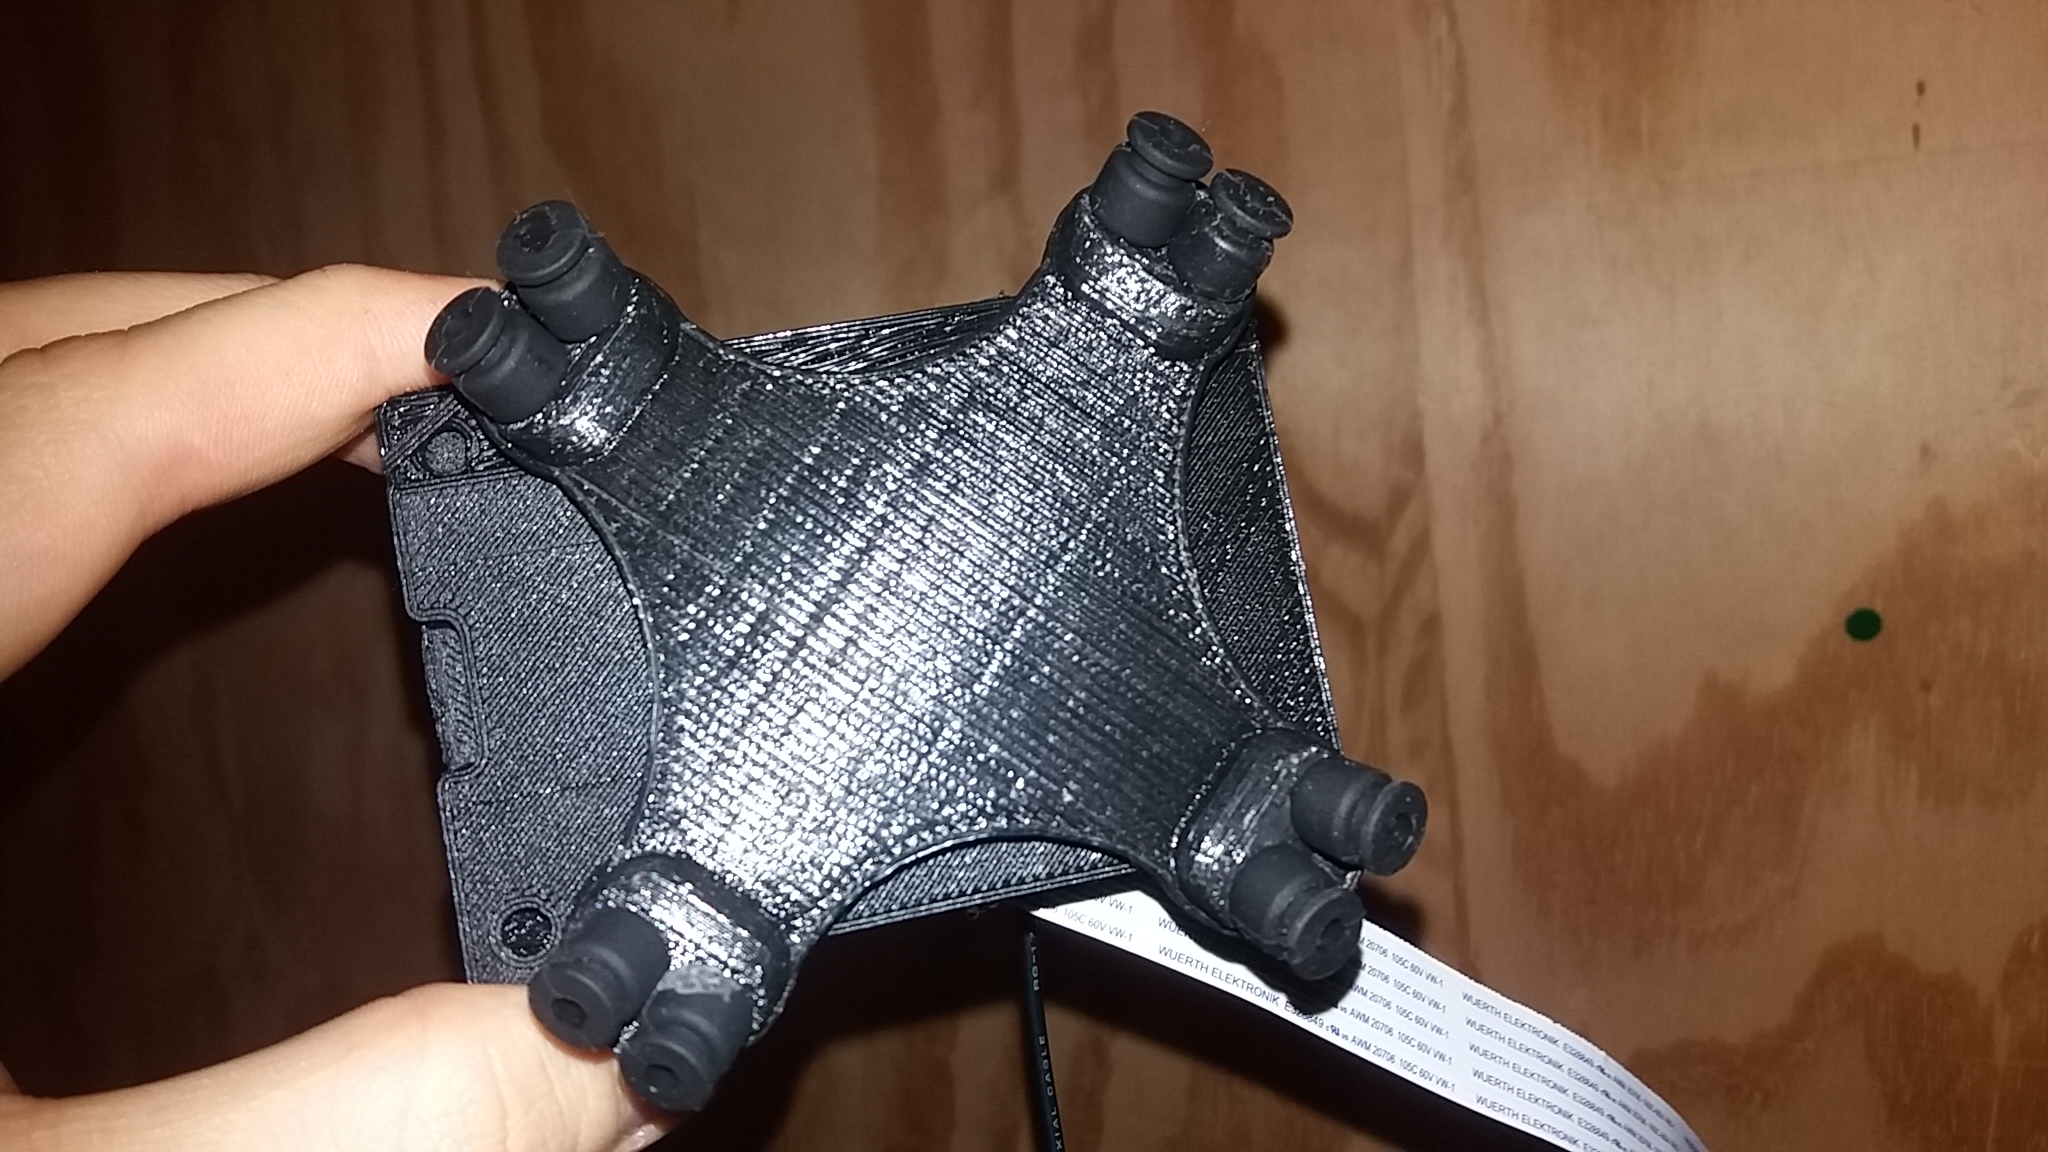
\includegraphics[scale=0.1]{images/drone-build-damper-balls.jpg}
\caption{Rubber vibration damper balls for platform.}
\label{fig:balls}
\end{subfigure}
\caption{Isolating vibrations between flight controller and the rest of the drone}
\label{fig:stabilize_platform}
\end{figure}

One of the biggest problems in a drone is the vibrations emanating from the motors, travelling along the frame and affecting the flight controller. If not isolated from the flight controller, they induce a disturbance to the PID loop since the accuracy of the gyroscope, accelerometer and barometer readings are affected. In some cases, disturbed more than the PID loop can reasonably determine the current state of the drone.\\

Thus, damper balls can be used to isolate vibrations significantly from the flight controller.

\begin{figure}[H]
\begin{subfigure}{0.5\textwidth}
\centering
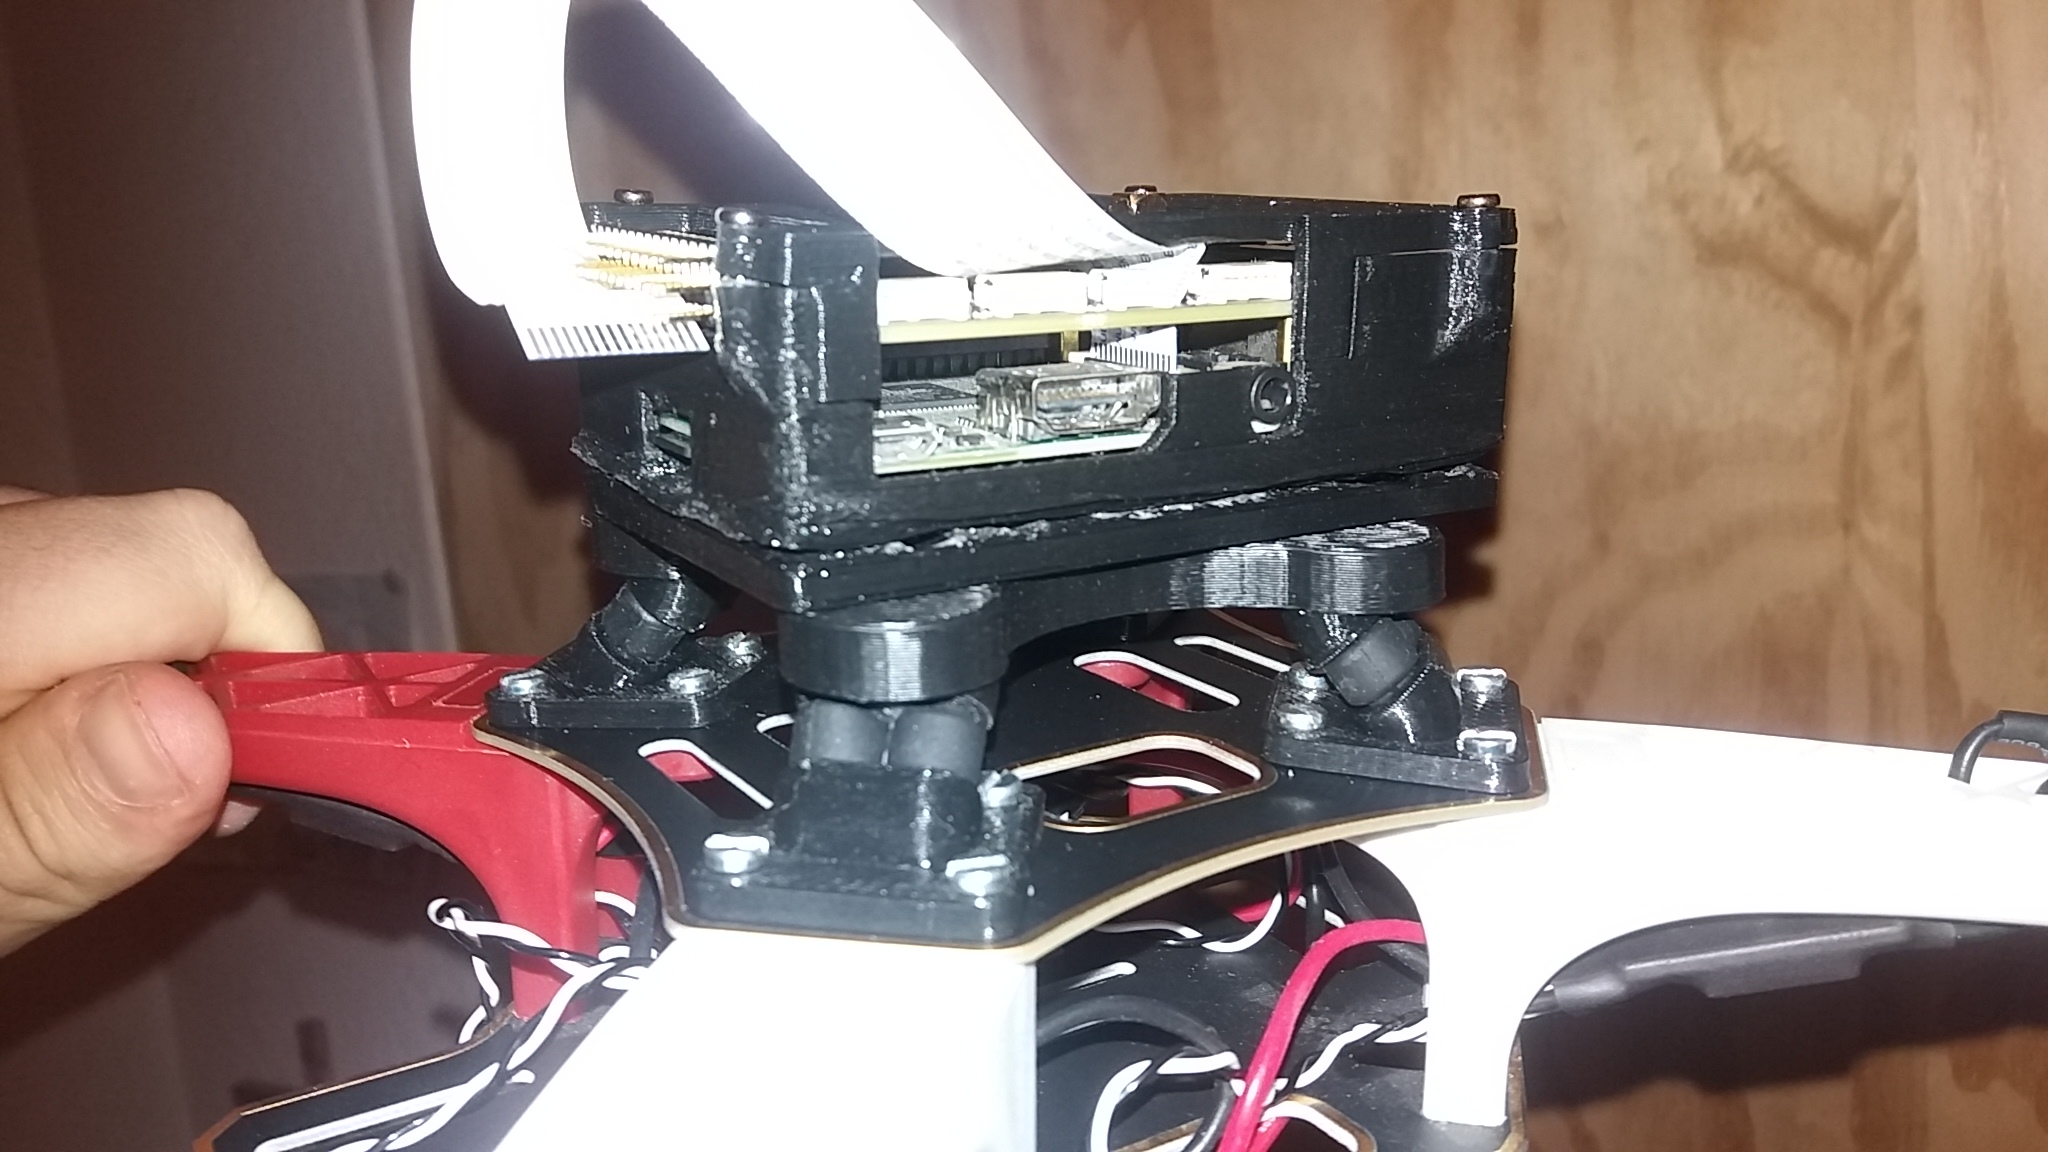
\includegraphics[scale=0.1]{images/drone-build-case-ondrone.jpg}
\caption{Attaching 3D printed case and platform to drone.}
\label{fig:attach_case_drone}
\end{subfigure}
\begin{subfigure}{0.5\textwidth}
\centering
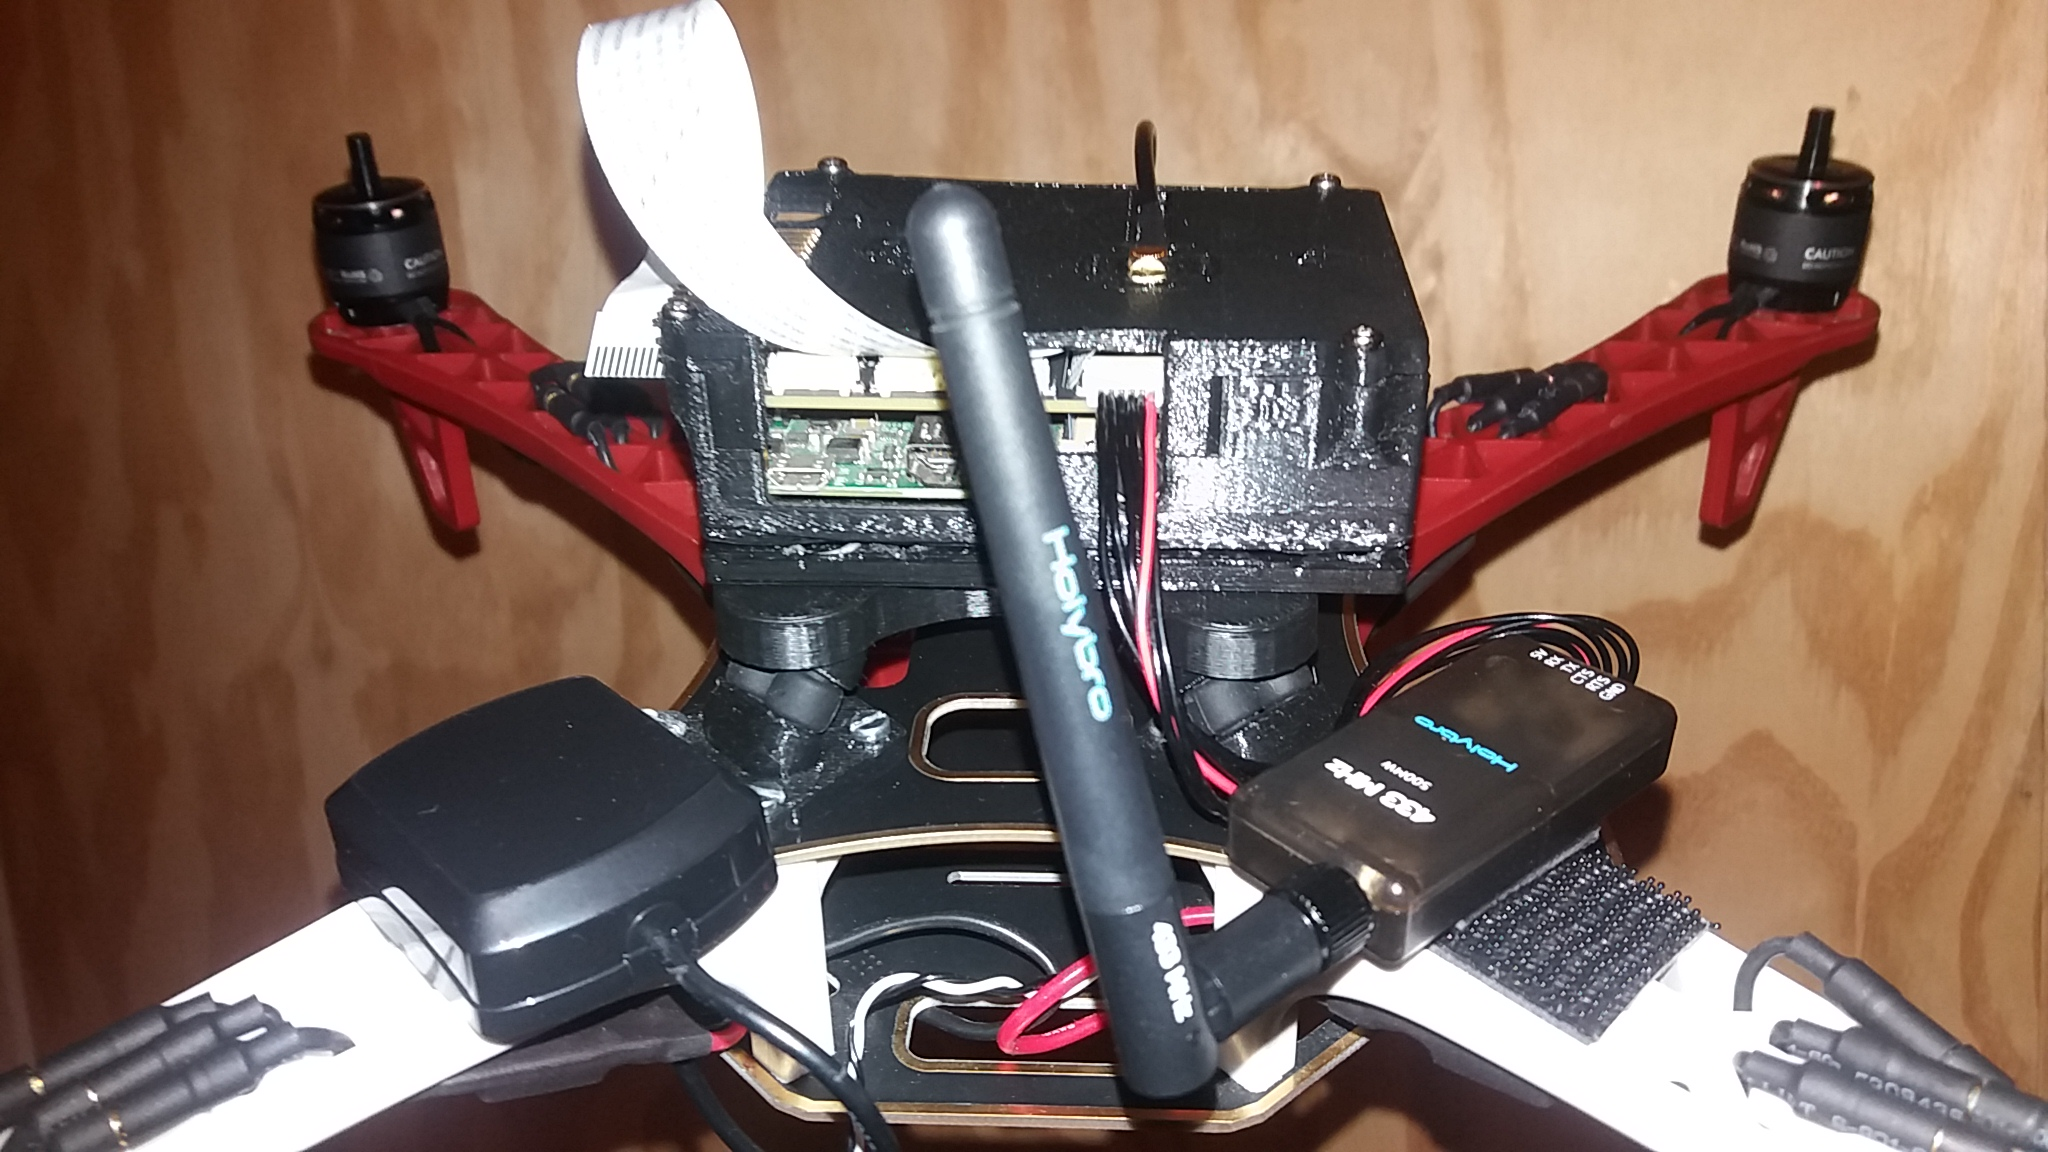
\includegraphics[scale=0.1]{images/drone-build-433.jpg}
\caption{Adding 433MHz telemtery to drone.}
\label{fig:attach_433}
\end{subfigure}
\caption{Adding telemetry and flight controller}
\label{fig:attach_case_433}
\end{figure}

\begin{figure}[H]
\begin{subfigure}{0.5\textwidth}
\centering
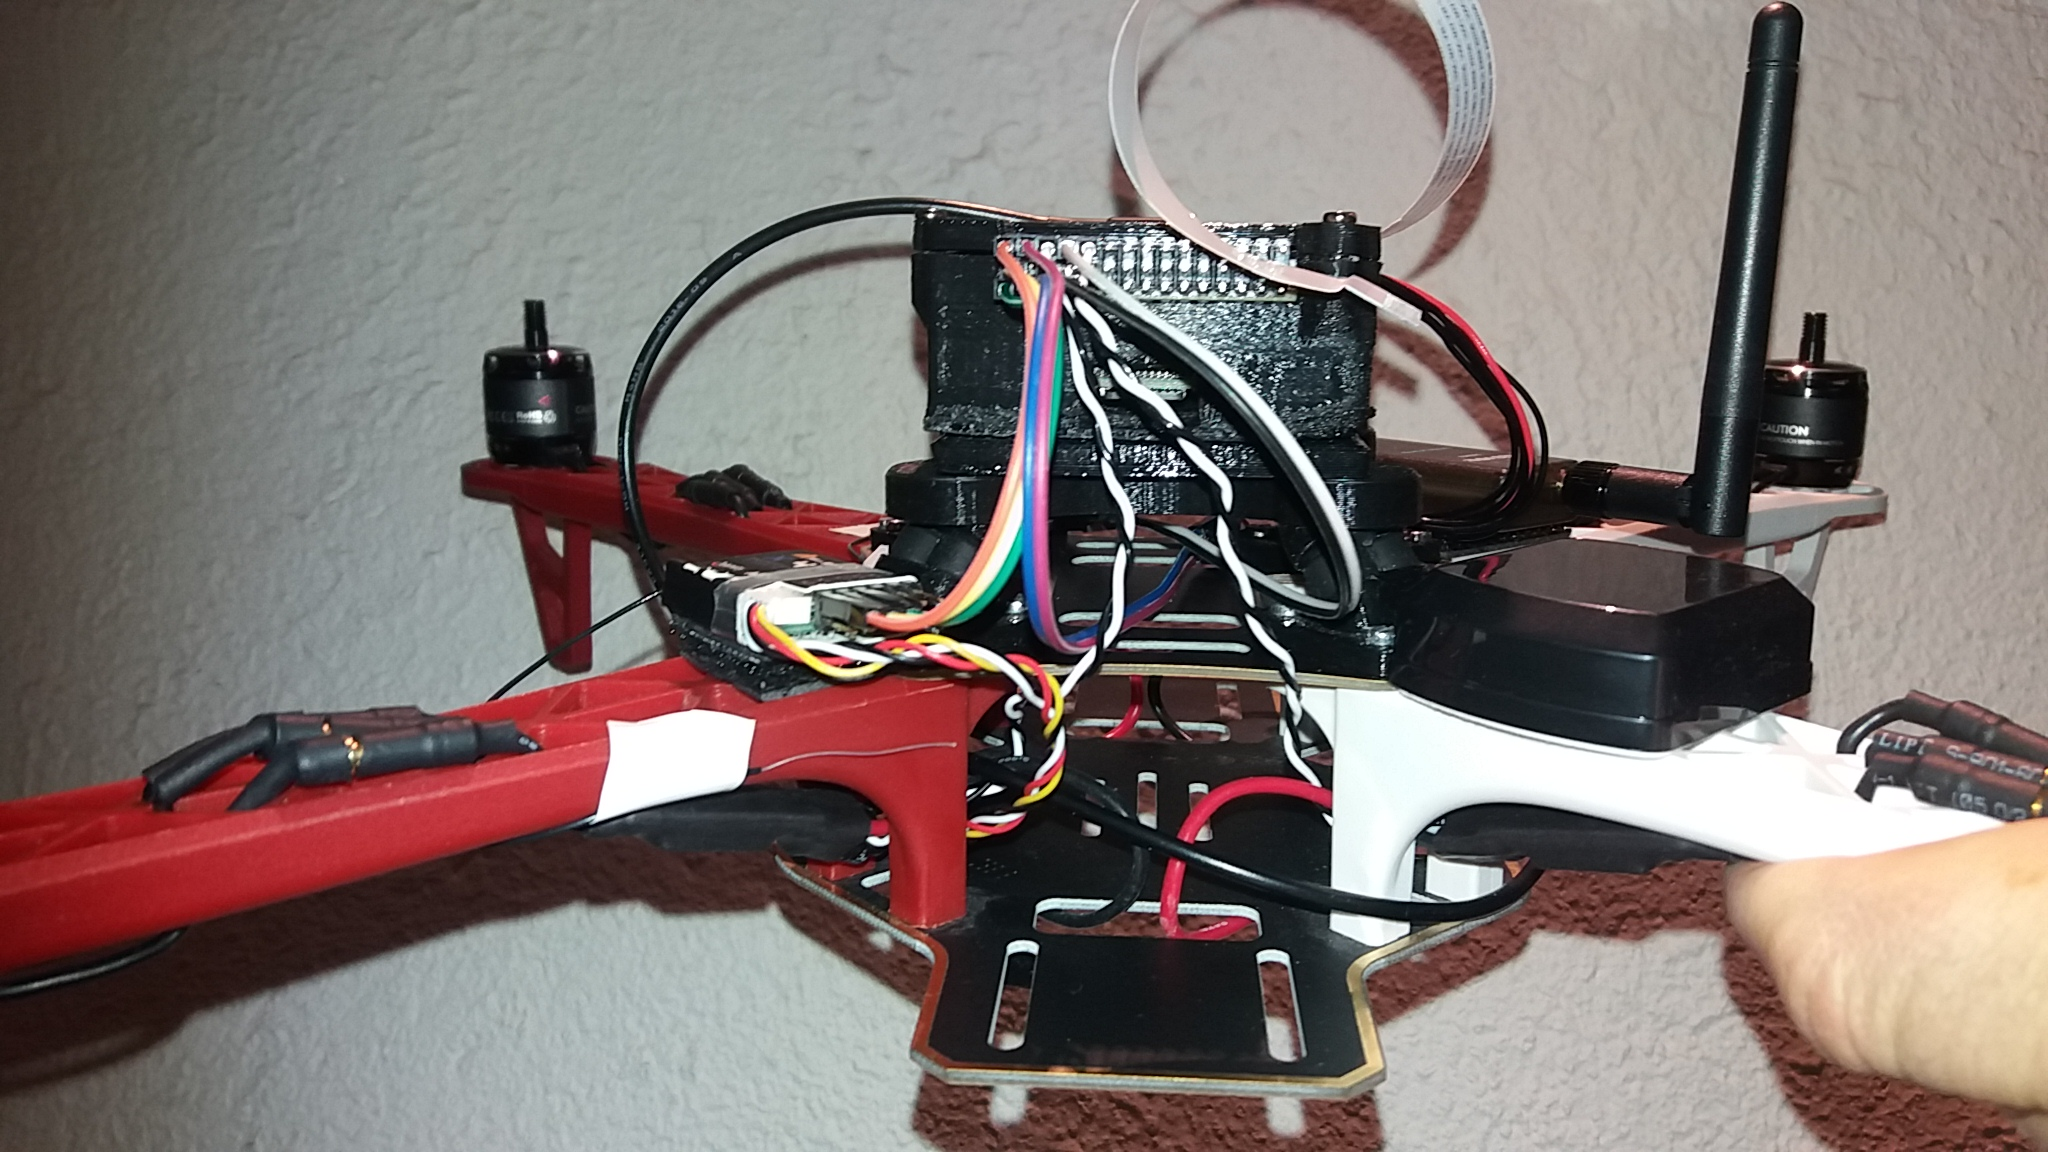
\includegraphics[scale=0.1]{images/drone-build-signal-wires.jpg}
\caption{Wiring up the signal wires}
\label{fig:attach_sbus}
\end{subfigure}
\begin{subfigure}{0.5\textwidth}
\centering
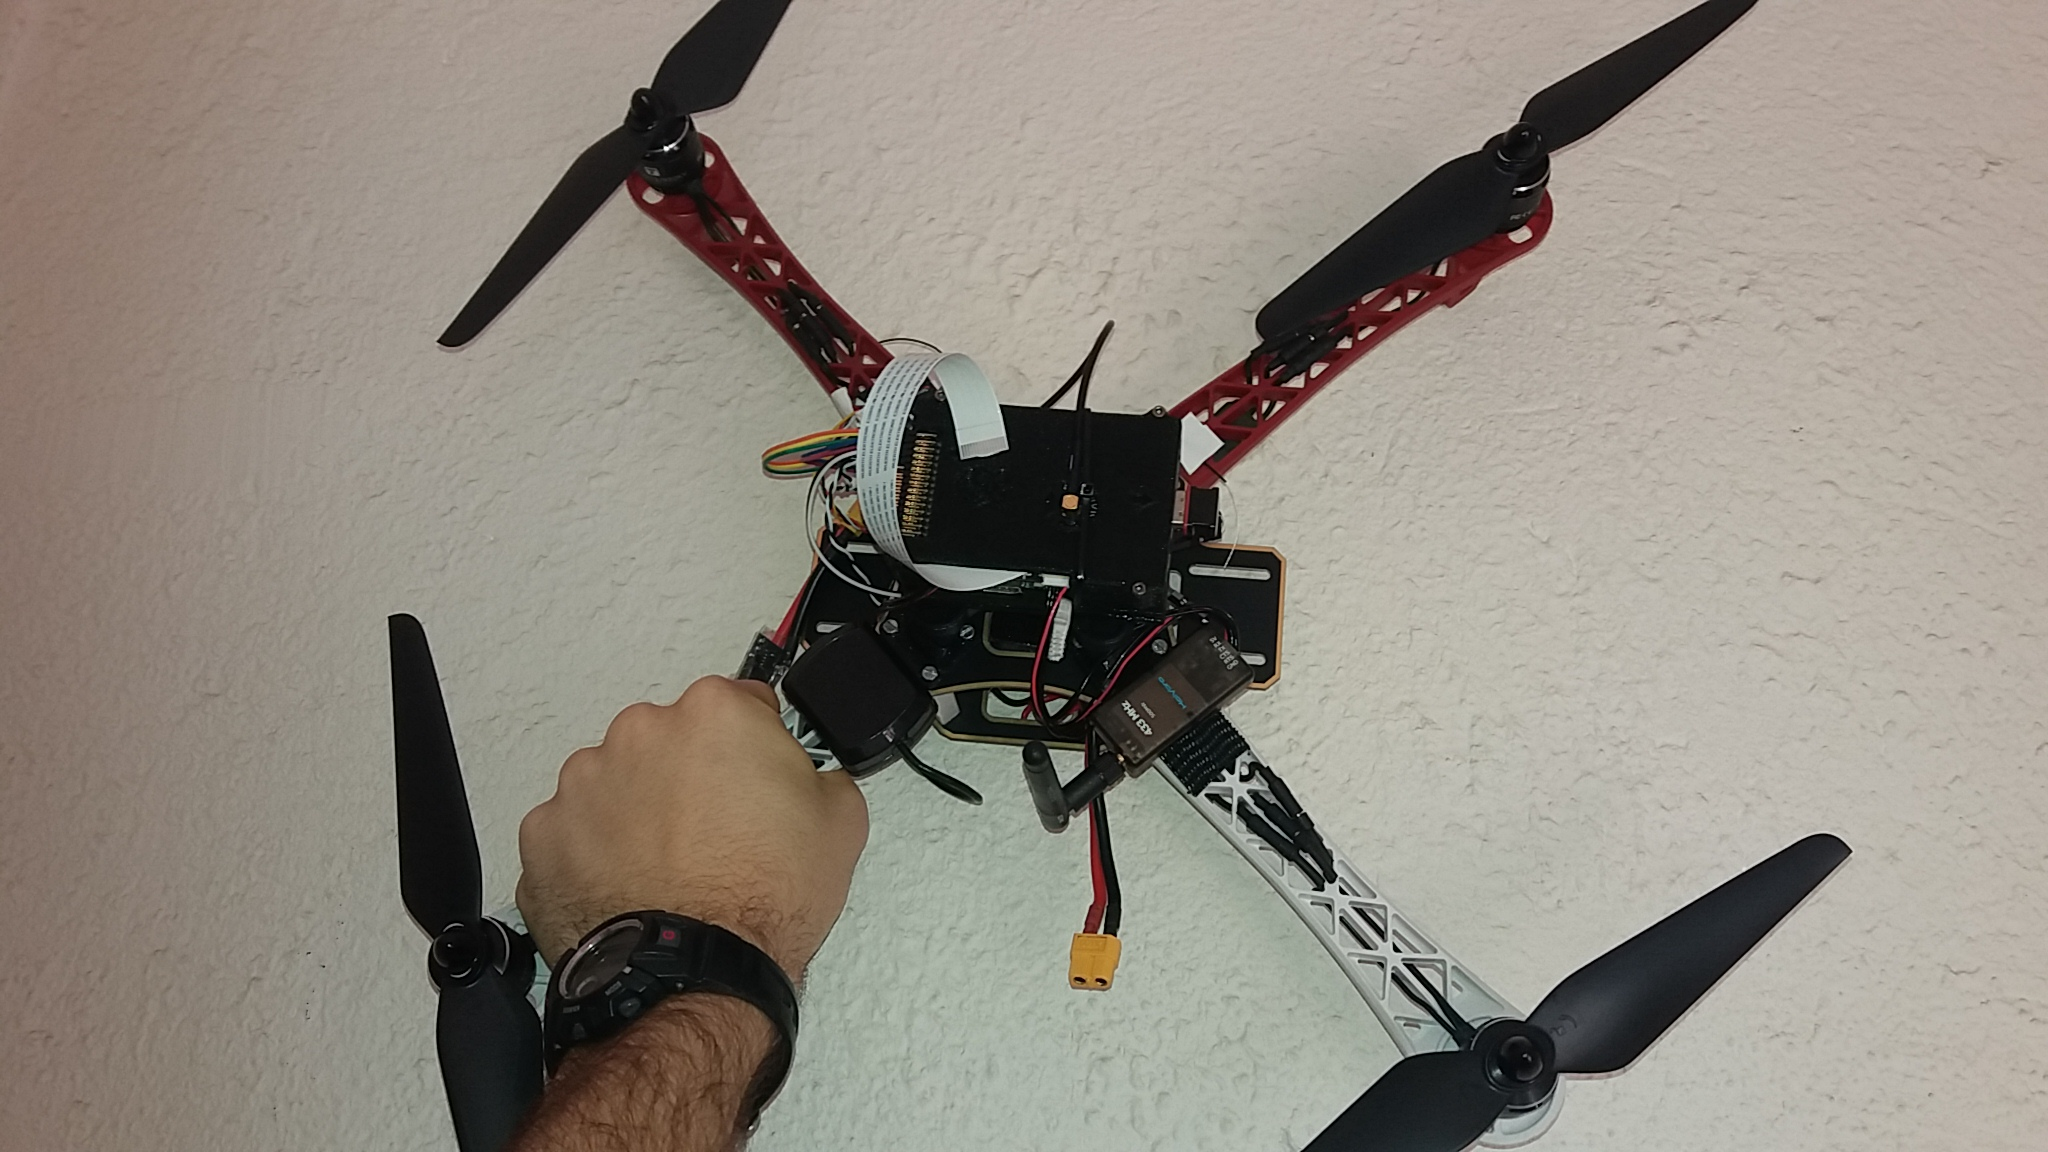
\includegraphics[scale=0.1]{images/drone-build-props.jpg}
\caption{Adding the 9.5'x4.5' propellers}
\label{fig:attach_props}
\end{subfigure}
\caption{Ready to fly}
\label{fig:attach_signal_props}
\end{figure}

\section{Ground Control Station}

The GCS is necessary for pre-flight checks, monitoring/controlling the status of the vehicle during flight, and setting waypoints.\\

The drone communicates with the GCS in Figure \ref{fig:gcs} using 433 MHz transceivers as in Figure \ref{fig:attach_433}.

\begin{figure}[H]
\centering
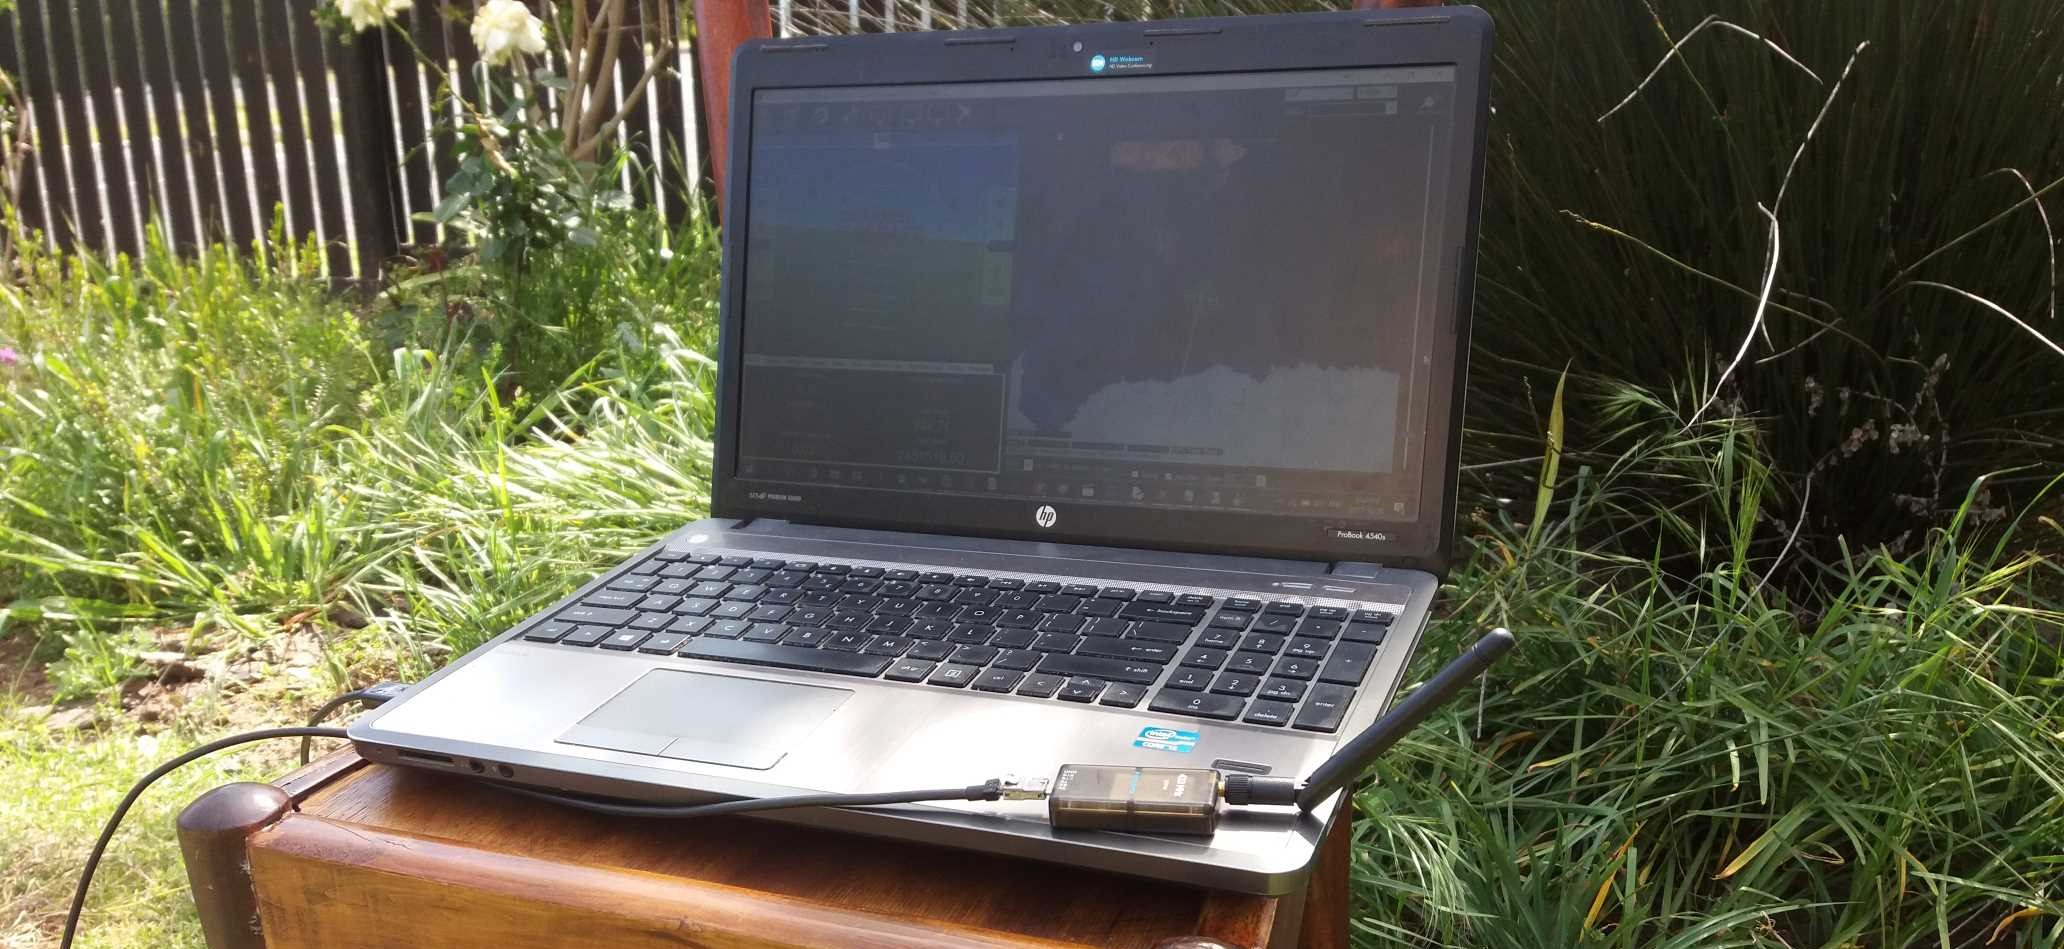
\includegraphics[scale=0.17]{images/gcs.jpg}
\caption{Ground Control Station}
\label{fig:gcs}
\end{figure}

The software used is the open source Mission Planner platform.

\begin{figure}[H]
\centering
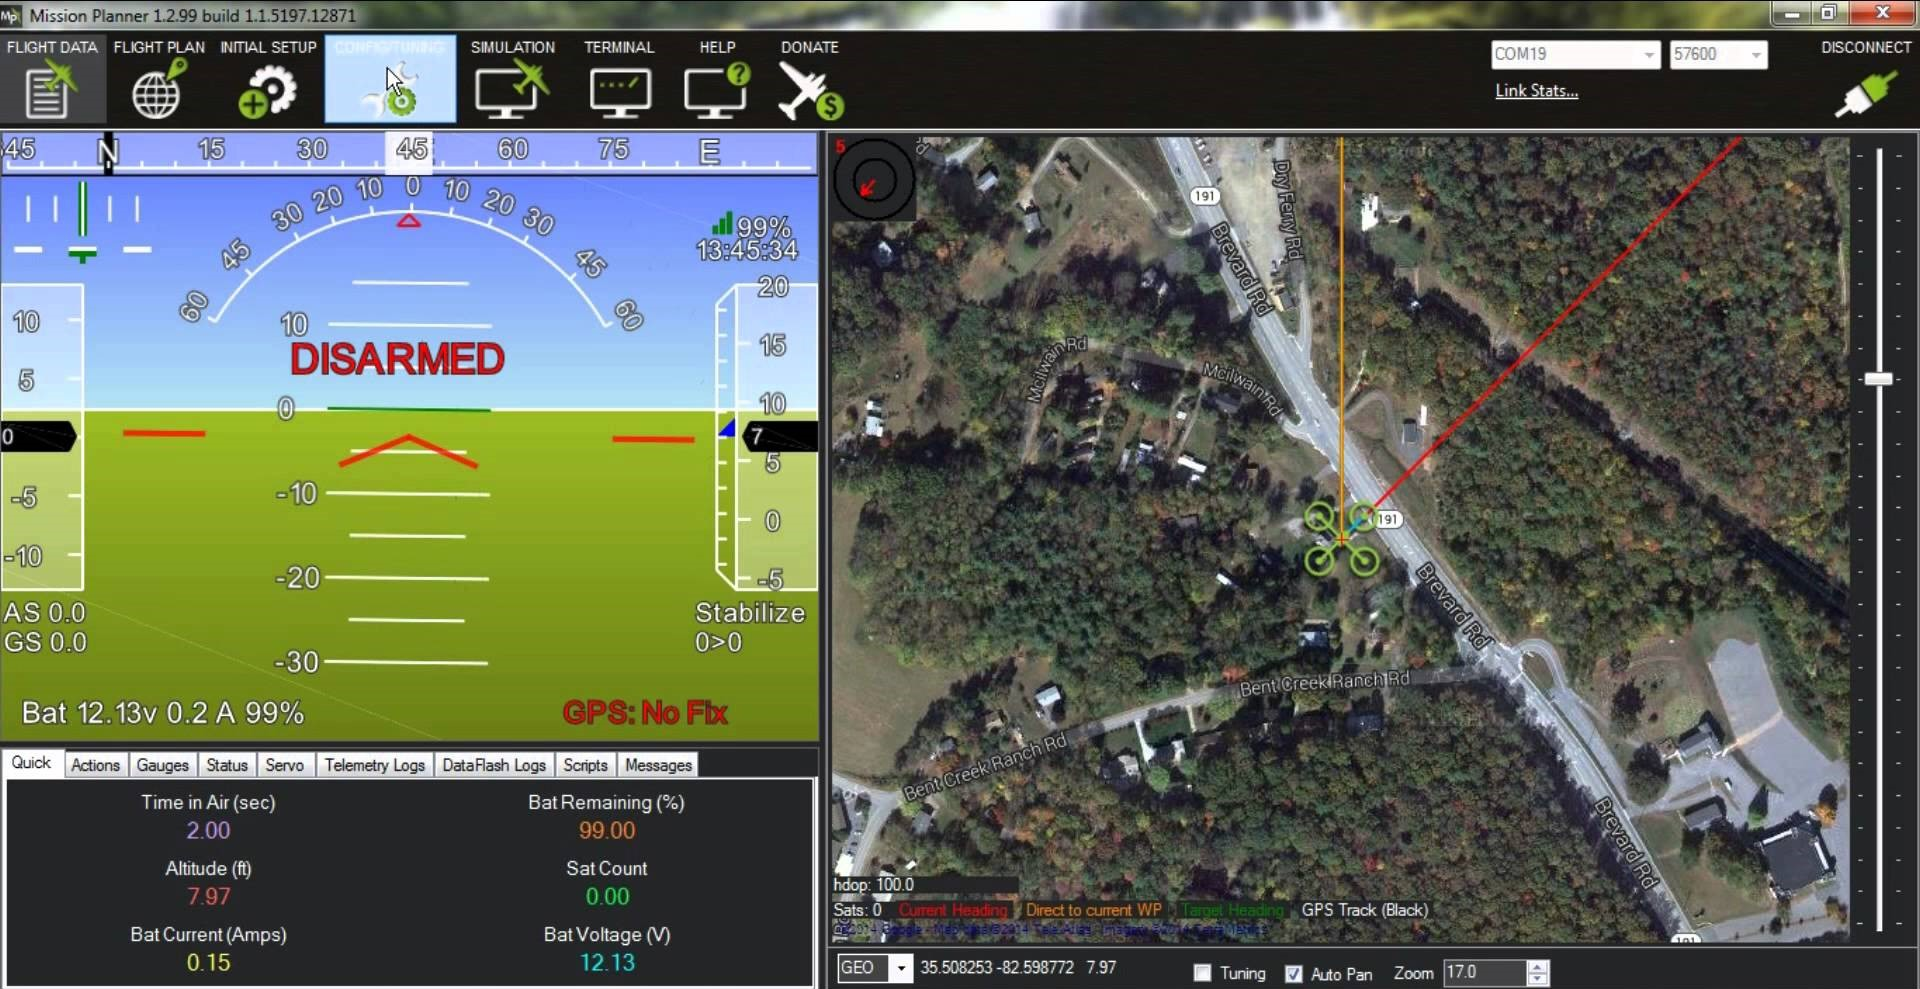
\includegraphics[scale=0.2]{images/mp.jpg}
\caption{Mission planner}
\label{fig:mission_planner}
\end{figure}

\section{Remote controller}
\label{sec:remote_controller}

The remote controller is used to manually control the drone. It is also used to monitor the battery and signal strength.\\

\begin{figure}[H]
\begin{subfigure}{0.5\textwidth}
\centering
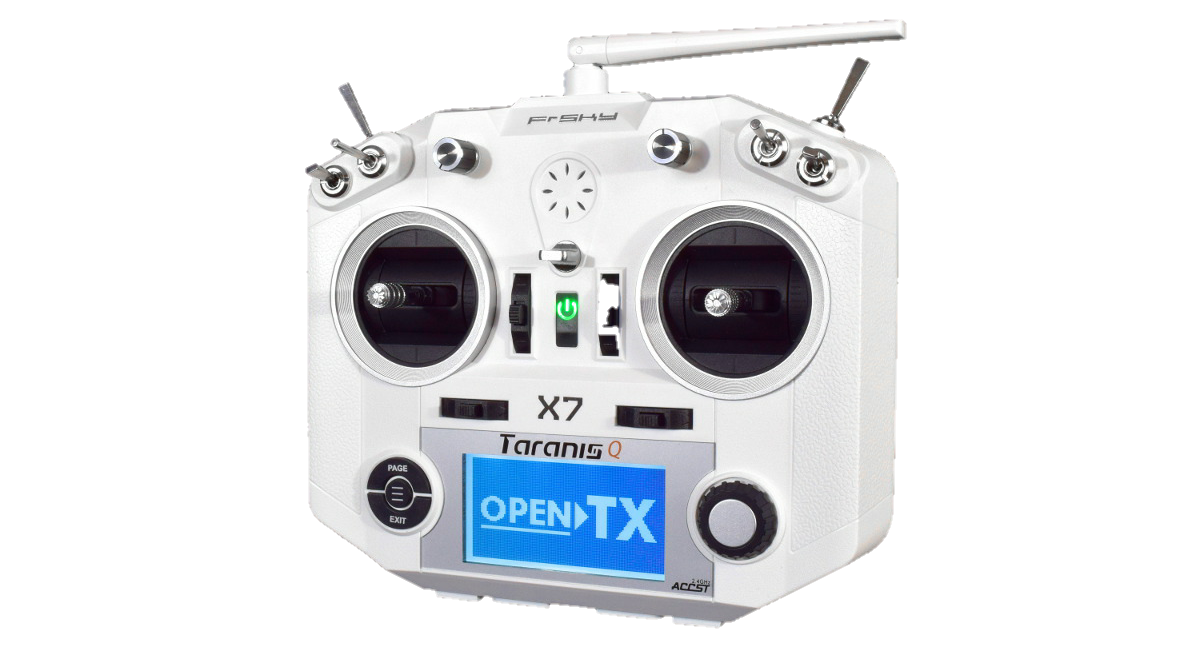
\includegraphics[scale=0.255]{images/taranis.png}
\caption{Taranis Q X7 remote controller}
\label{fig:remote_controller}
\end{subfigure}
\begin{subfigure}{0.5\textwidth}
\centering
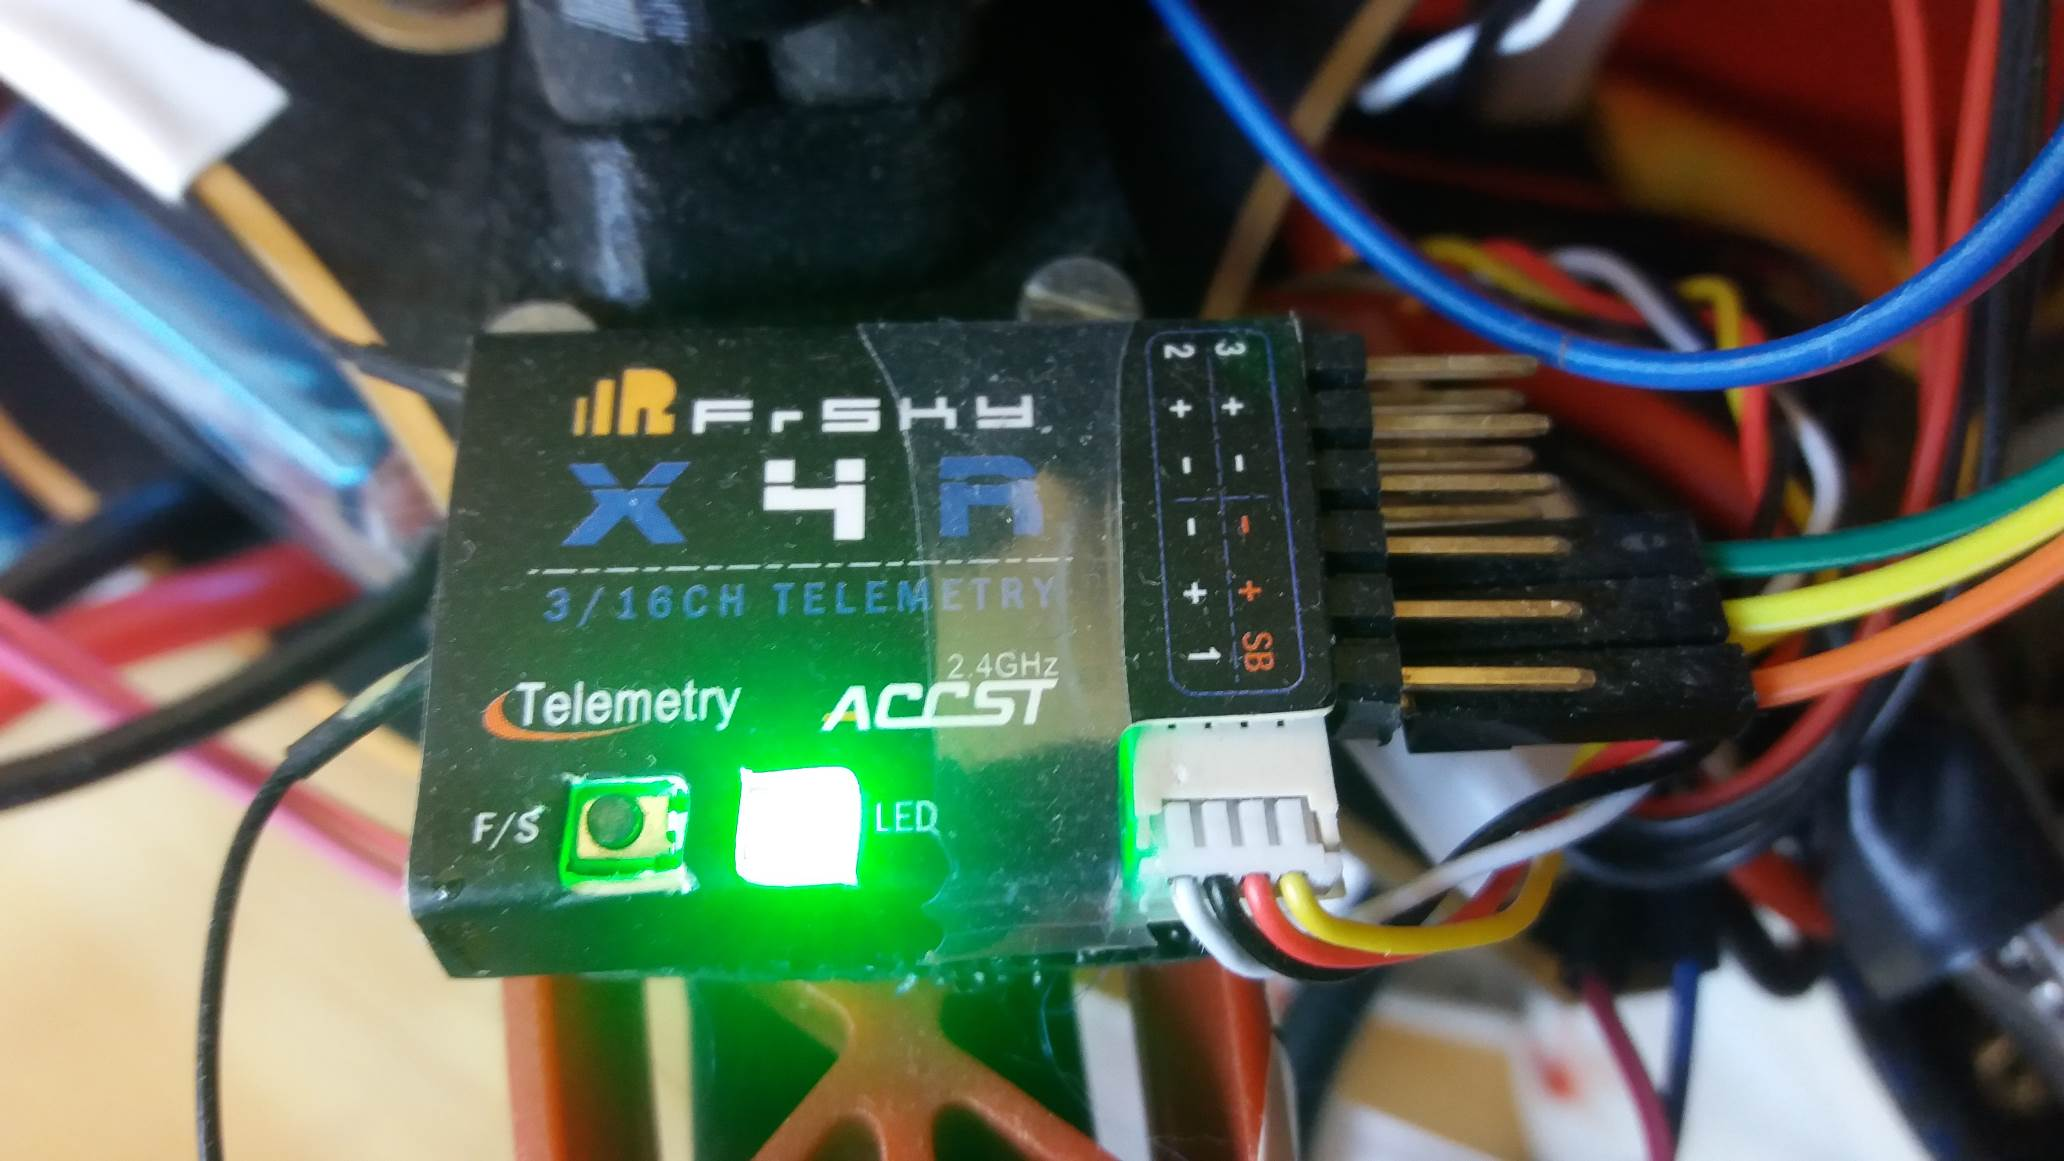
\includegraphics[scale=0.15]{images/frsky_transceiver.jpg}
\caption{FrSky X4R transceiver}
\label{fig:balls}
\end{subfigure}
\caption{Remote controller and on-board transceiver}
\label{fig:frsky_transceiver}
\end{figure}

The full-duplex remote controller outputs at 100mW. The FrSky X4R transceiver has two antennae, and also outputs at 100 mW.\\

At first, the Taranis remote controller is bound to the FrSky X4R transceiver aboard the drone in Figure \ref{fig:frsky_transceiver}. This is done by holding in the `F\/S' button on the transceiver while powering it on, and entering bind mode on the remote controller.

\begin{figure}[H]
\begin{subfigure}{0.5\textwidth}
\centering
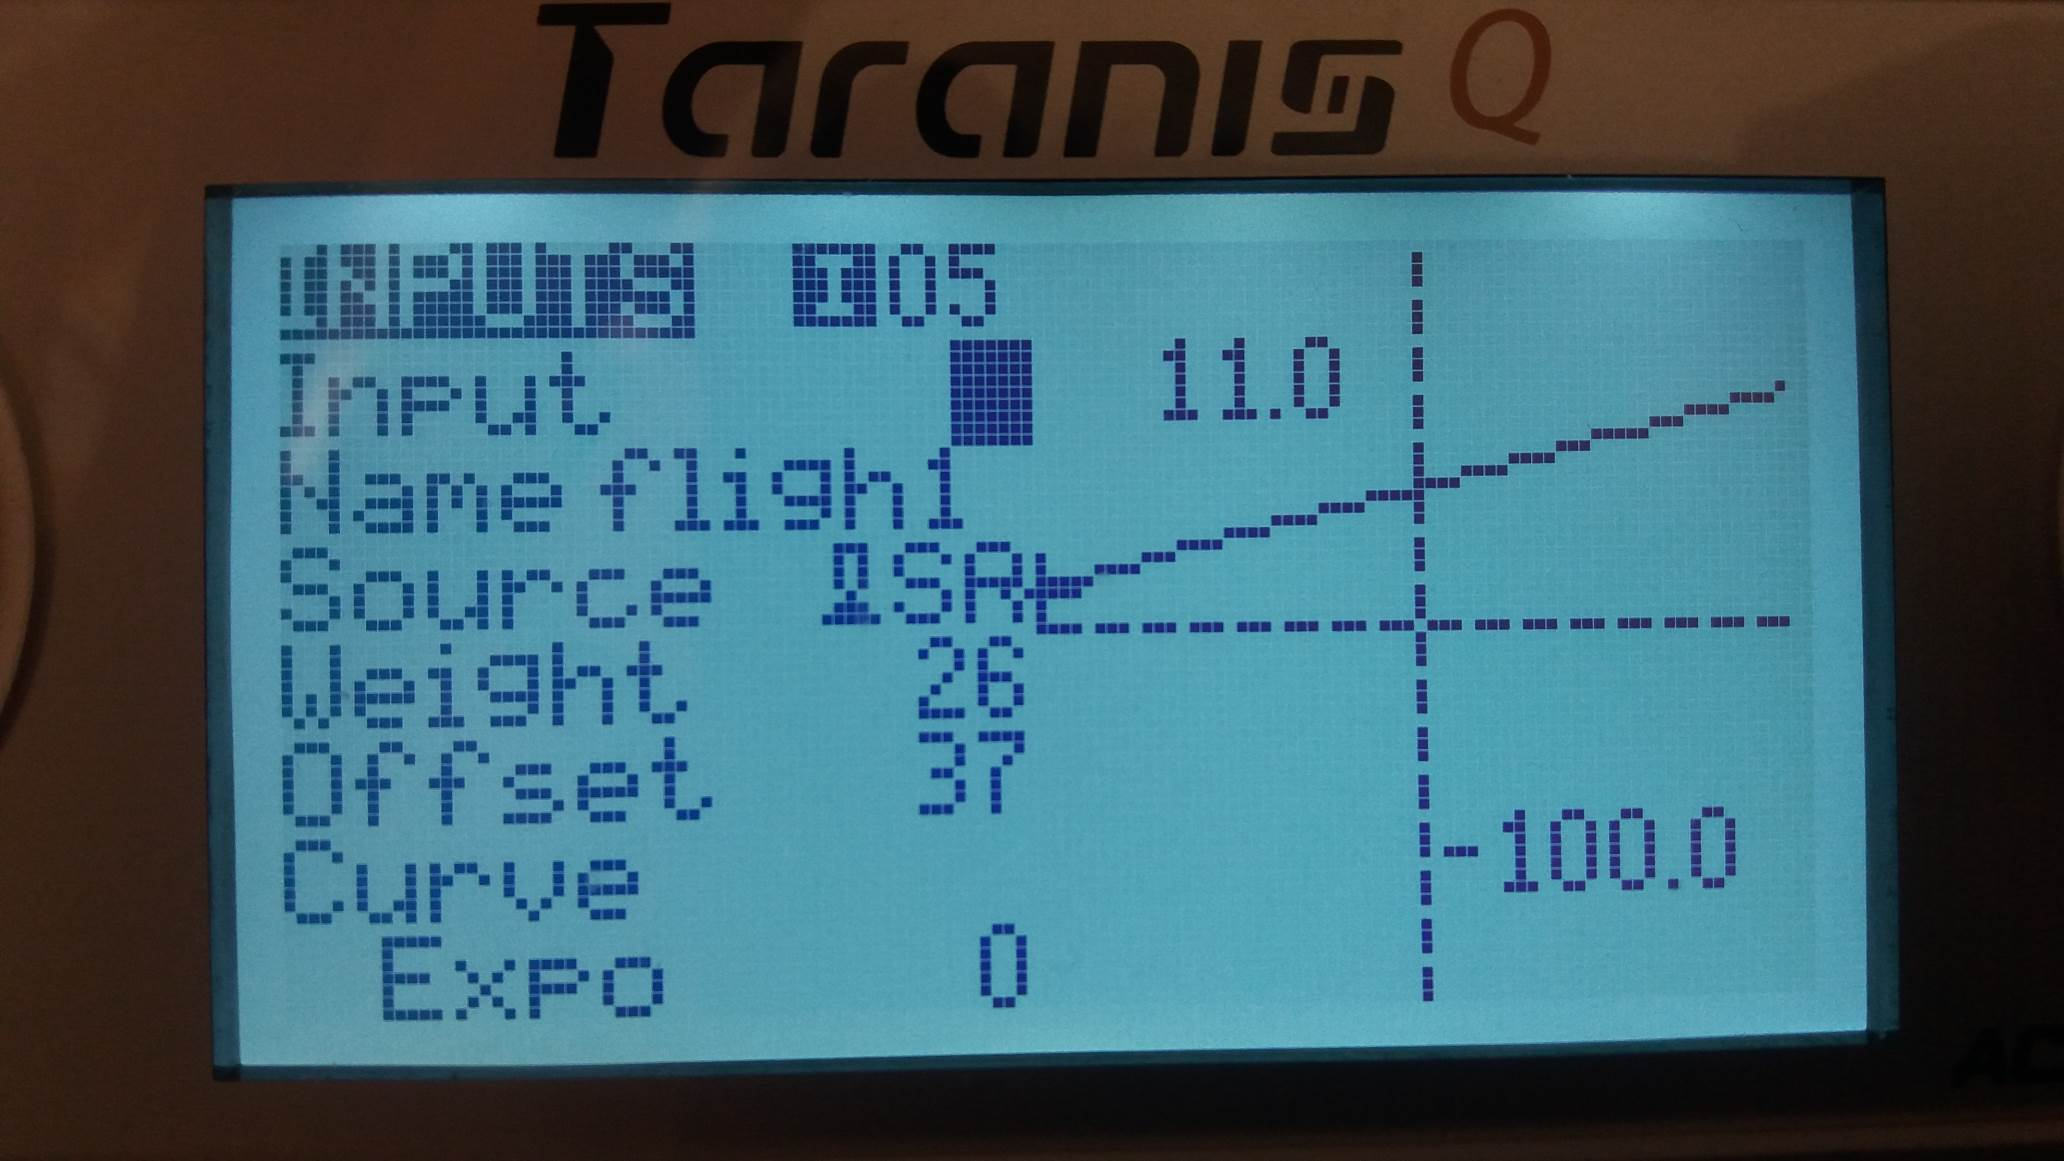
\includegraphics[scale=0.13]{images/lcd/flight_mode_but_1.jpg}
\caption{Linearised flight mode switch 1 input}
\label{fig:taranis_fm_but1}
\end{subfigure}
\begin{subfigure}{0.5\textwidth}
\centering
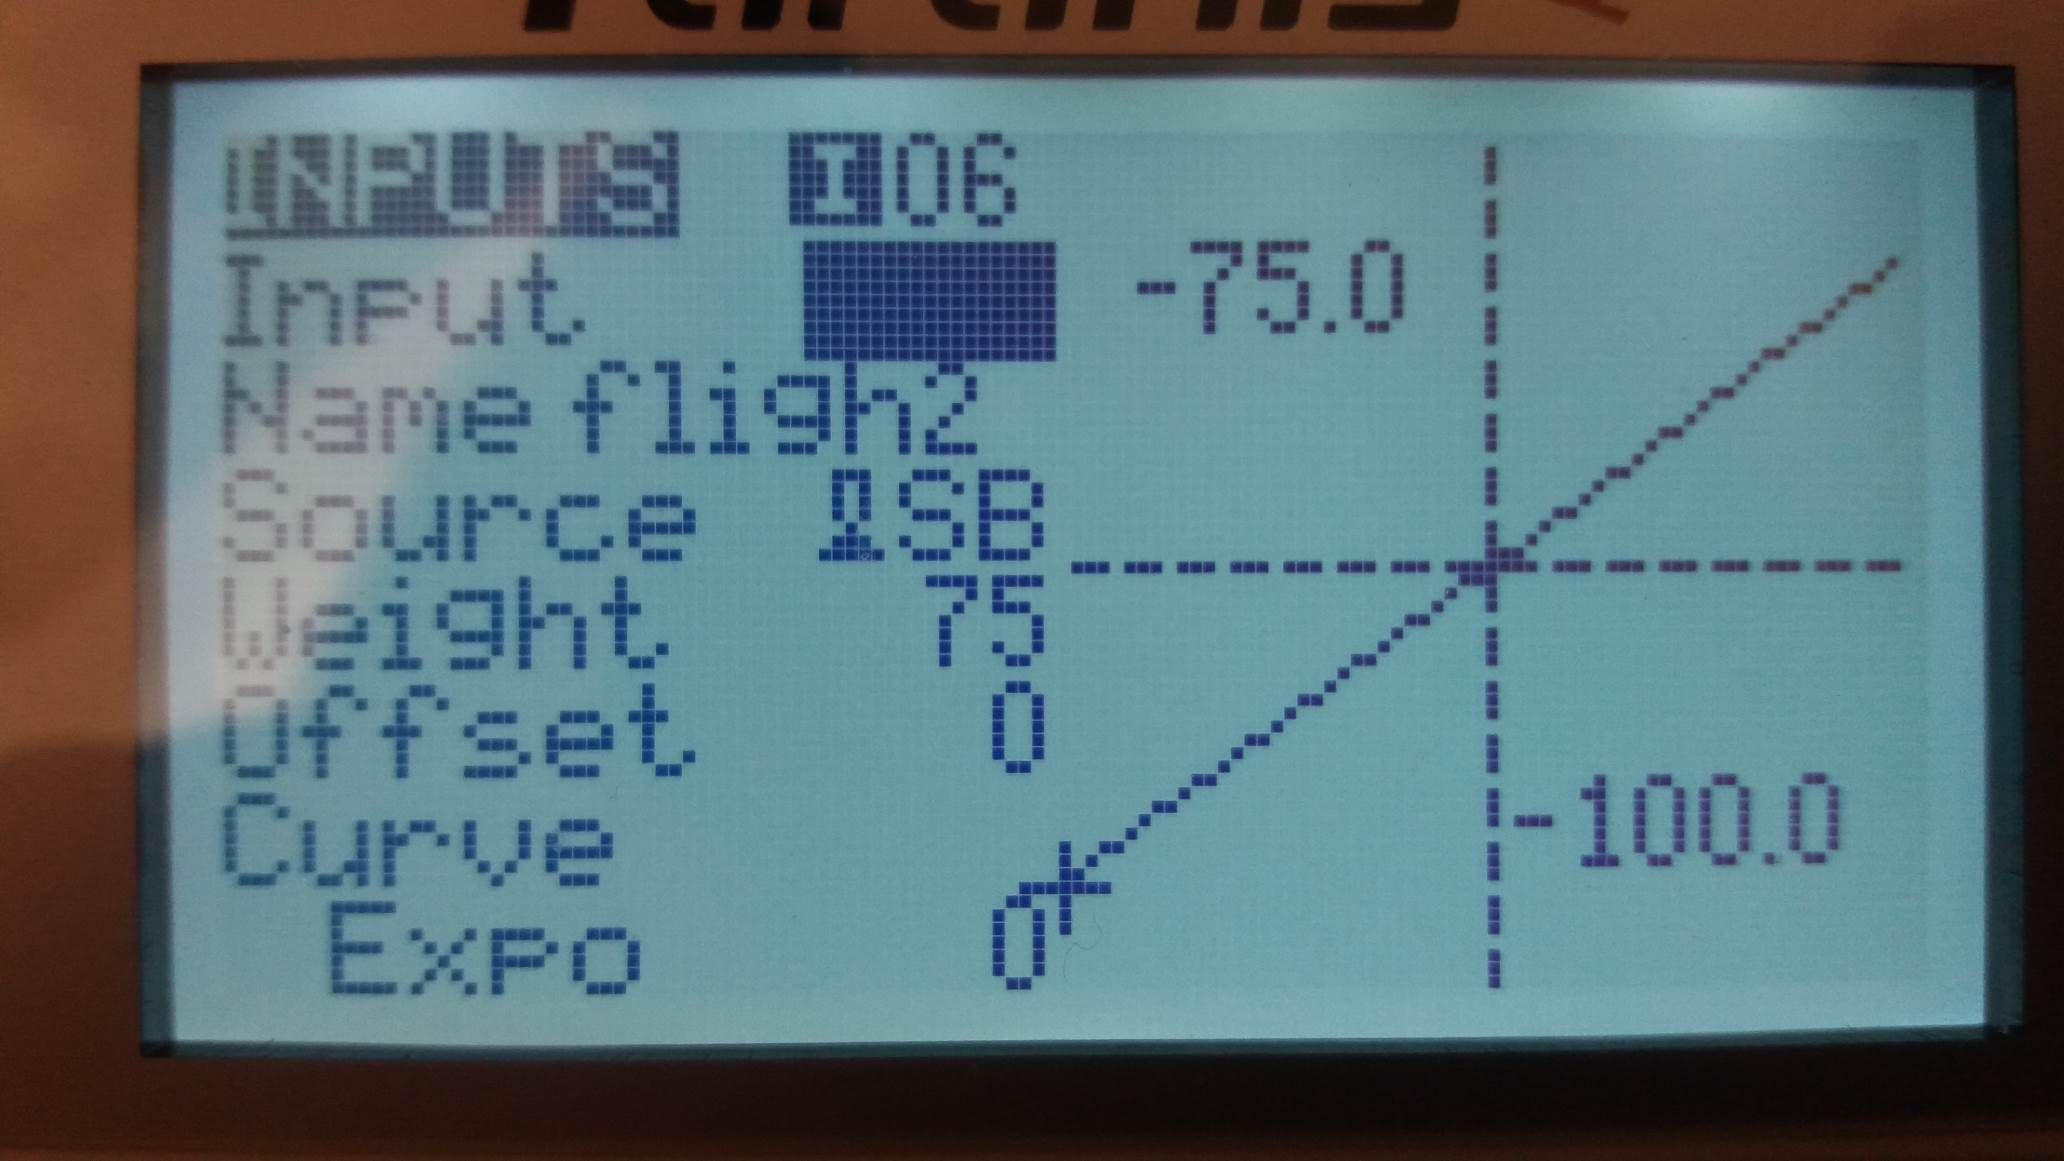
\includegraphics[scale=0.13]{images/lcd/flight_mode_but_2.jpg}
\caption{Linearised flight mode switch 2 input}
\label{fig:taranis_fm_but2}
\end{subfigure}
\begin{subfigure}{0.5\textwidth}
\centering
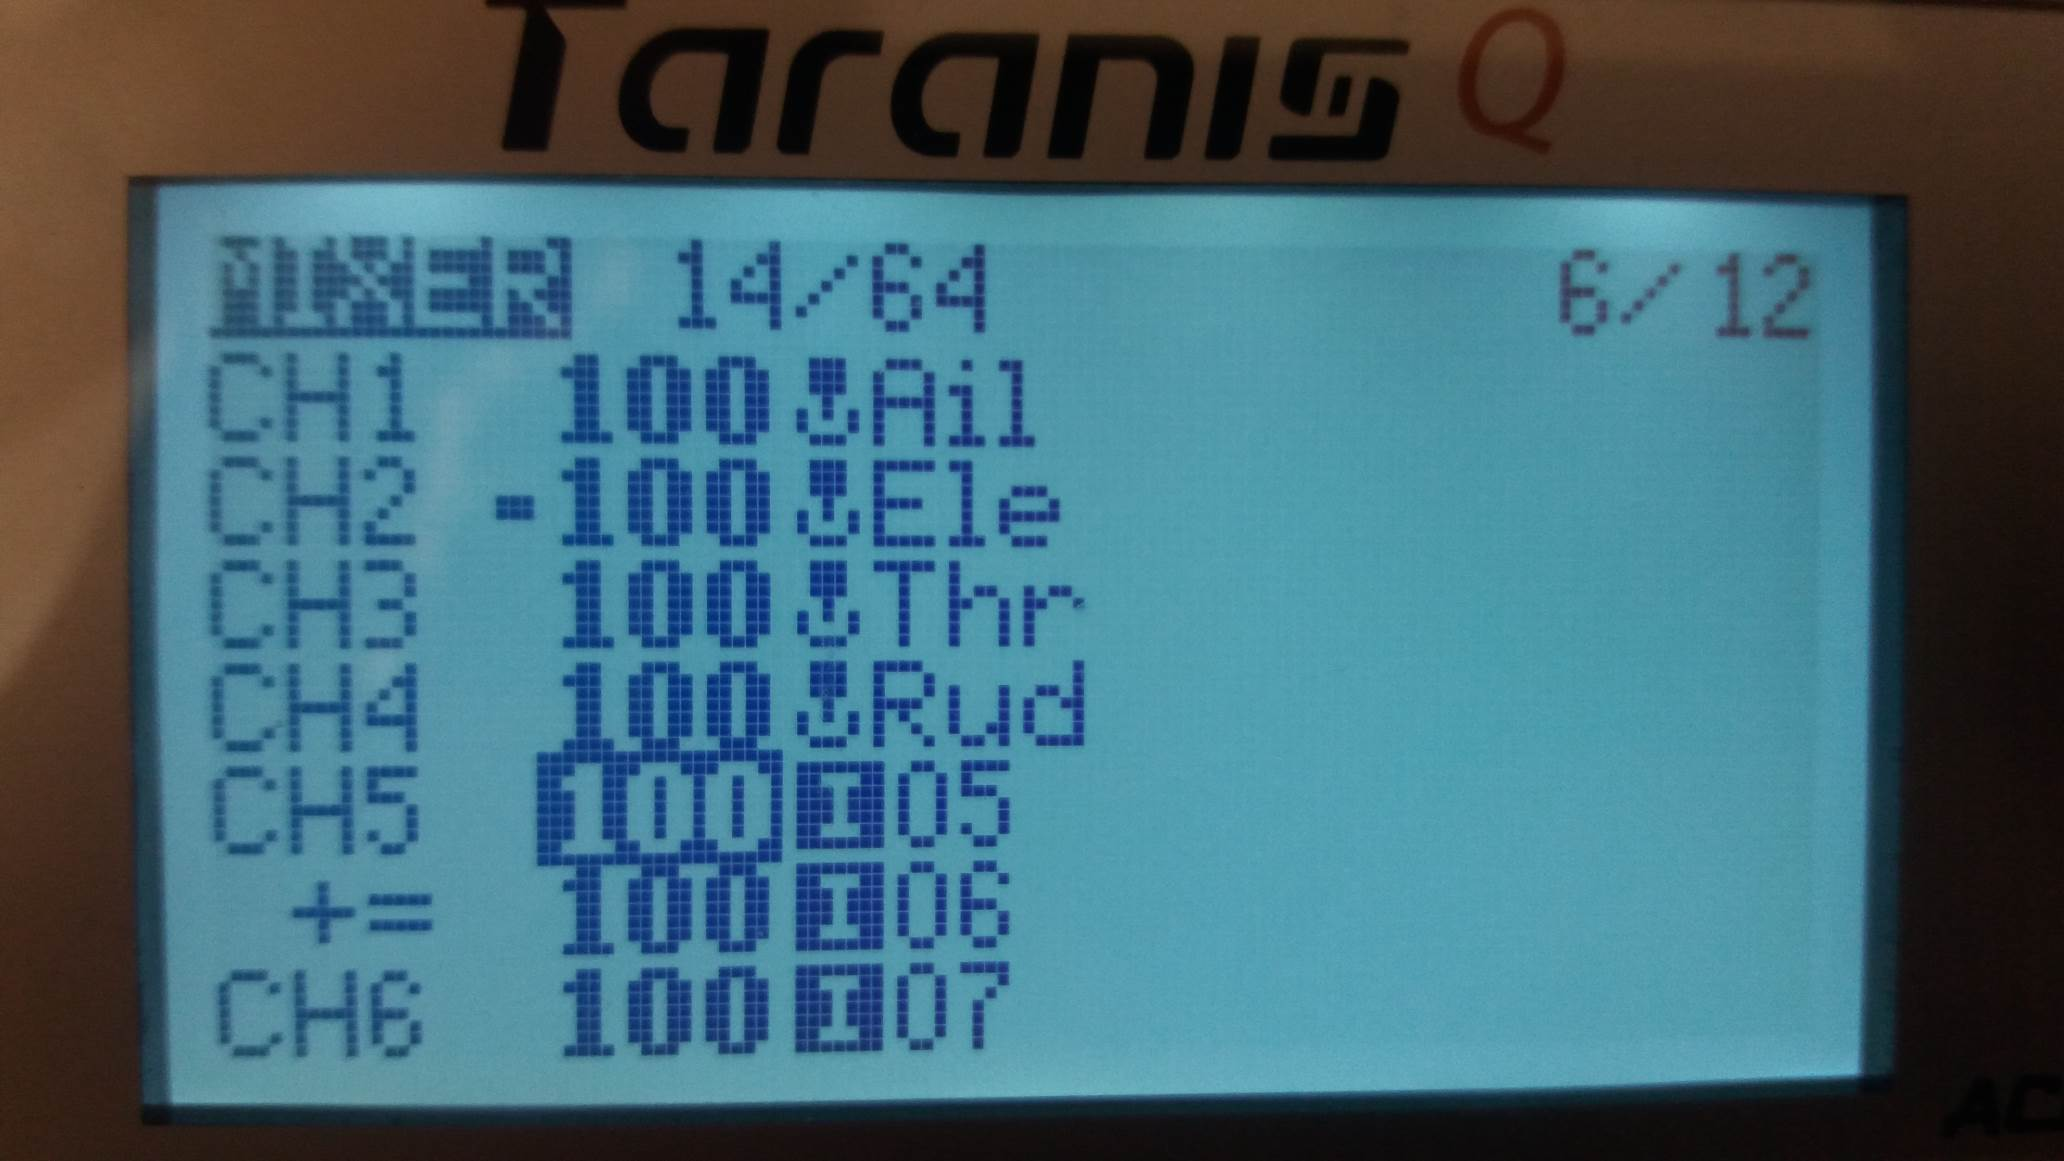
\includegraphics[scale=0.13]{images/lcd/mixer.jpg}
\caption{Mixer muxes input channels to output}
\label{fig:taranis_mux}
\end{subfigure}
\begin{subfigure}{0.5\textwidth}
\centering
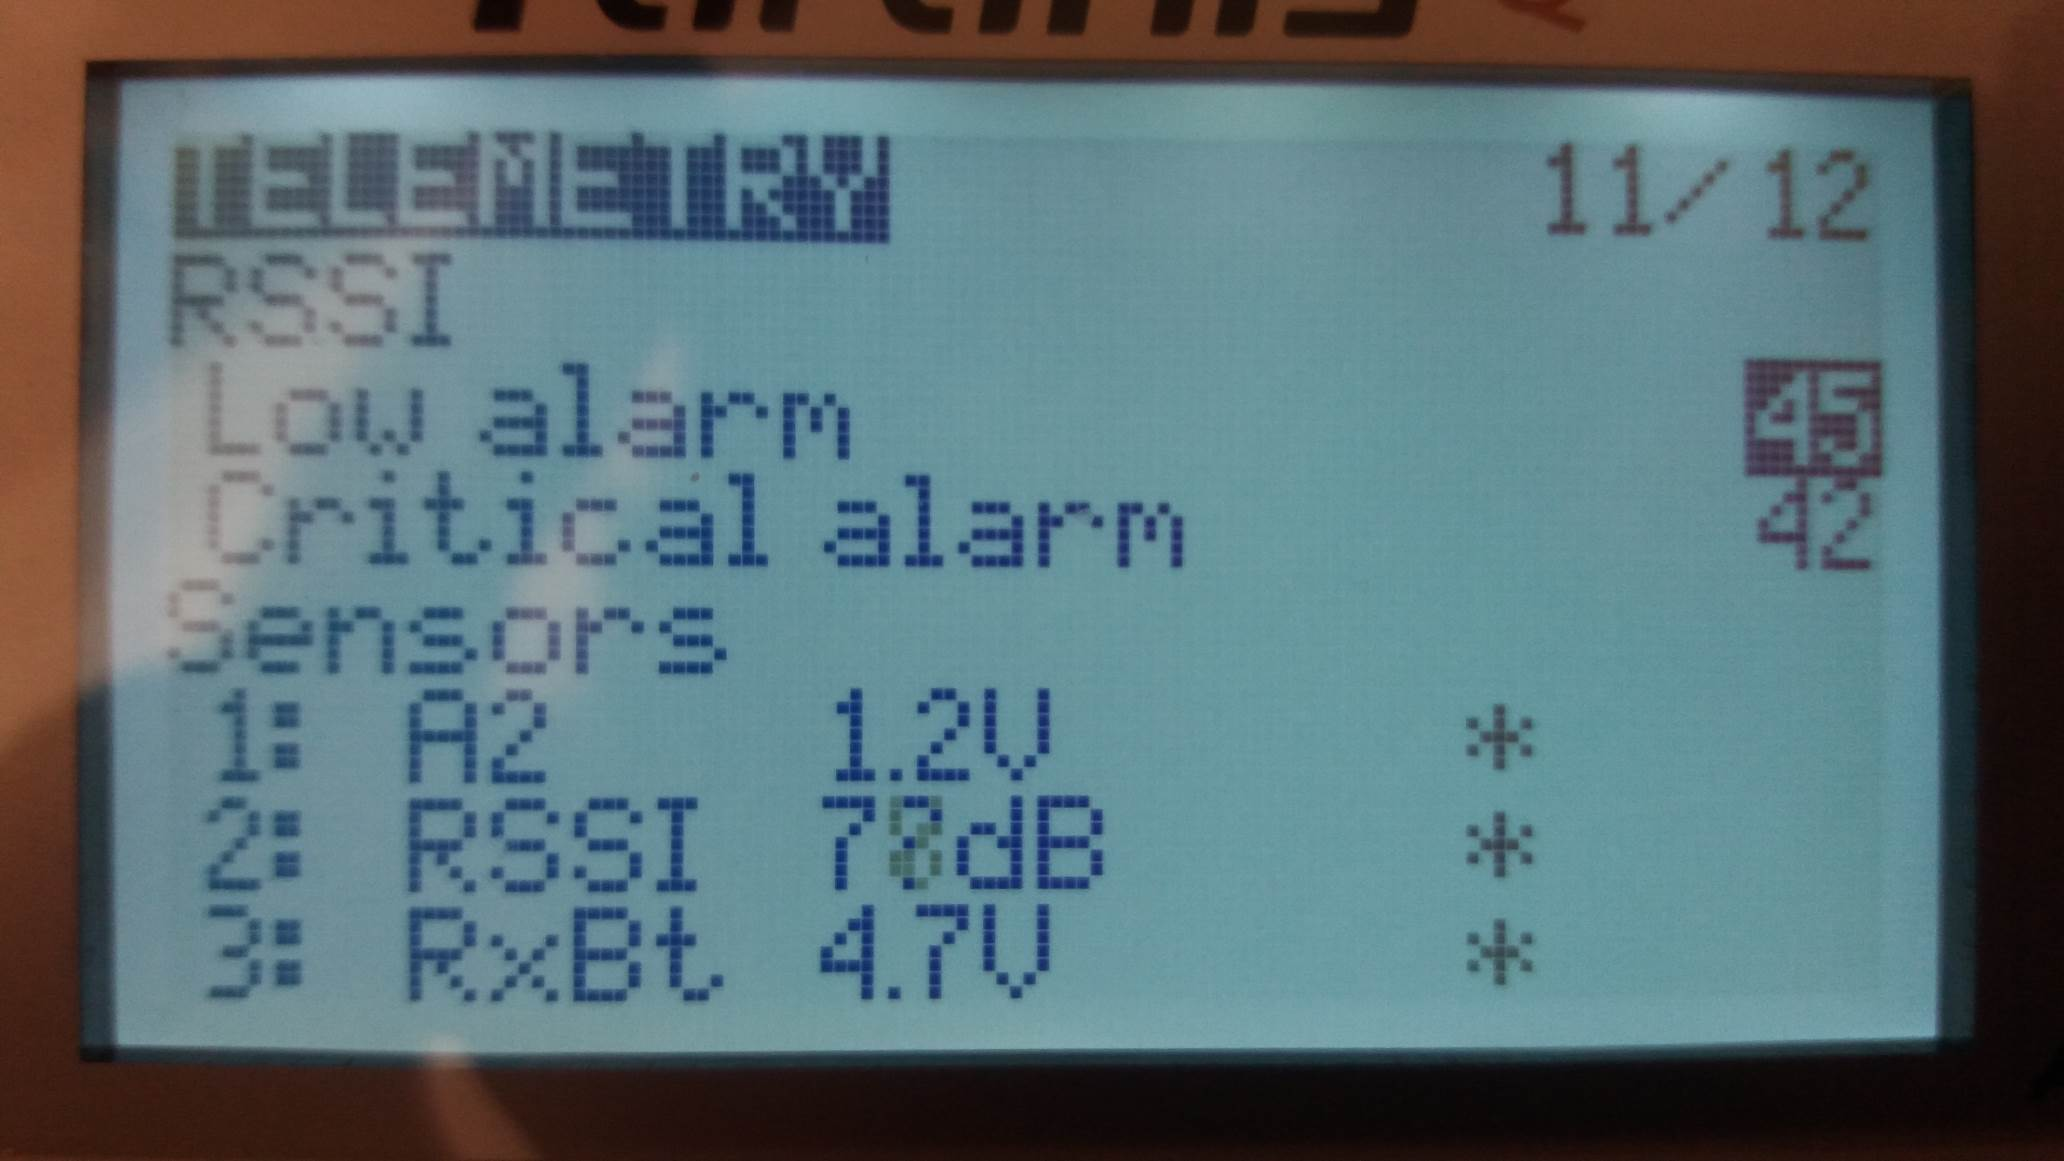
\includegraphics[scale=0.13]{images/lcd/telemetry.jpg}
\caption{Remote sensor feedback}
\label{fig:taranis_telemetry}
\end{subfigure}
\caption{Some important settings for the remote controller}
\label{fig:taranis_lcd}
\end{figure}

The two 3-way flight mode input switches as indicated in Figure \ref{fig:taranis_arm} are multiplexed into channel 5 as in Figure \ref{fig:taranis_mux}. As indicated in Figure \ref{fig:taranis_fm_but1} and \ref{fig:taranis_fm_but2}, the two switches required a peculiar linearisation such that when they are multiplexed, there exist 6 PWM positions within the duty cycle range. \begin{equation}PWM\ flight\ mode\ output\ values\ \in [1165, 1295, 1425, 1555, 1685, 1815]\ ms\end{equation}
This allows the PWM outputs to exist within the ranges as indicated in Figure \ref{fig:flight_modes}.

\begin{figure}[H]
\centering
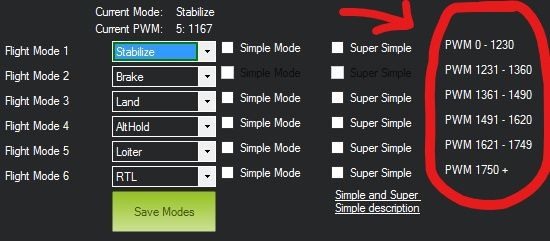
\includegraphics[scale=0.5]{images/flight_modes.JPG}
\caption{Flight modes}
\label{fig:flight_modes}
\end{figure}

To arm the drone for takeoff, move the left controller stick to the bottom right for 2 seconds, as in Figure \ref{fig:taranis_arm}. Also, lift the safety `Cut motors' switch.

\begin{figure}[H]
\centering
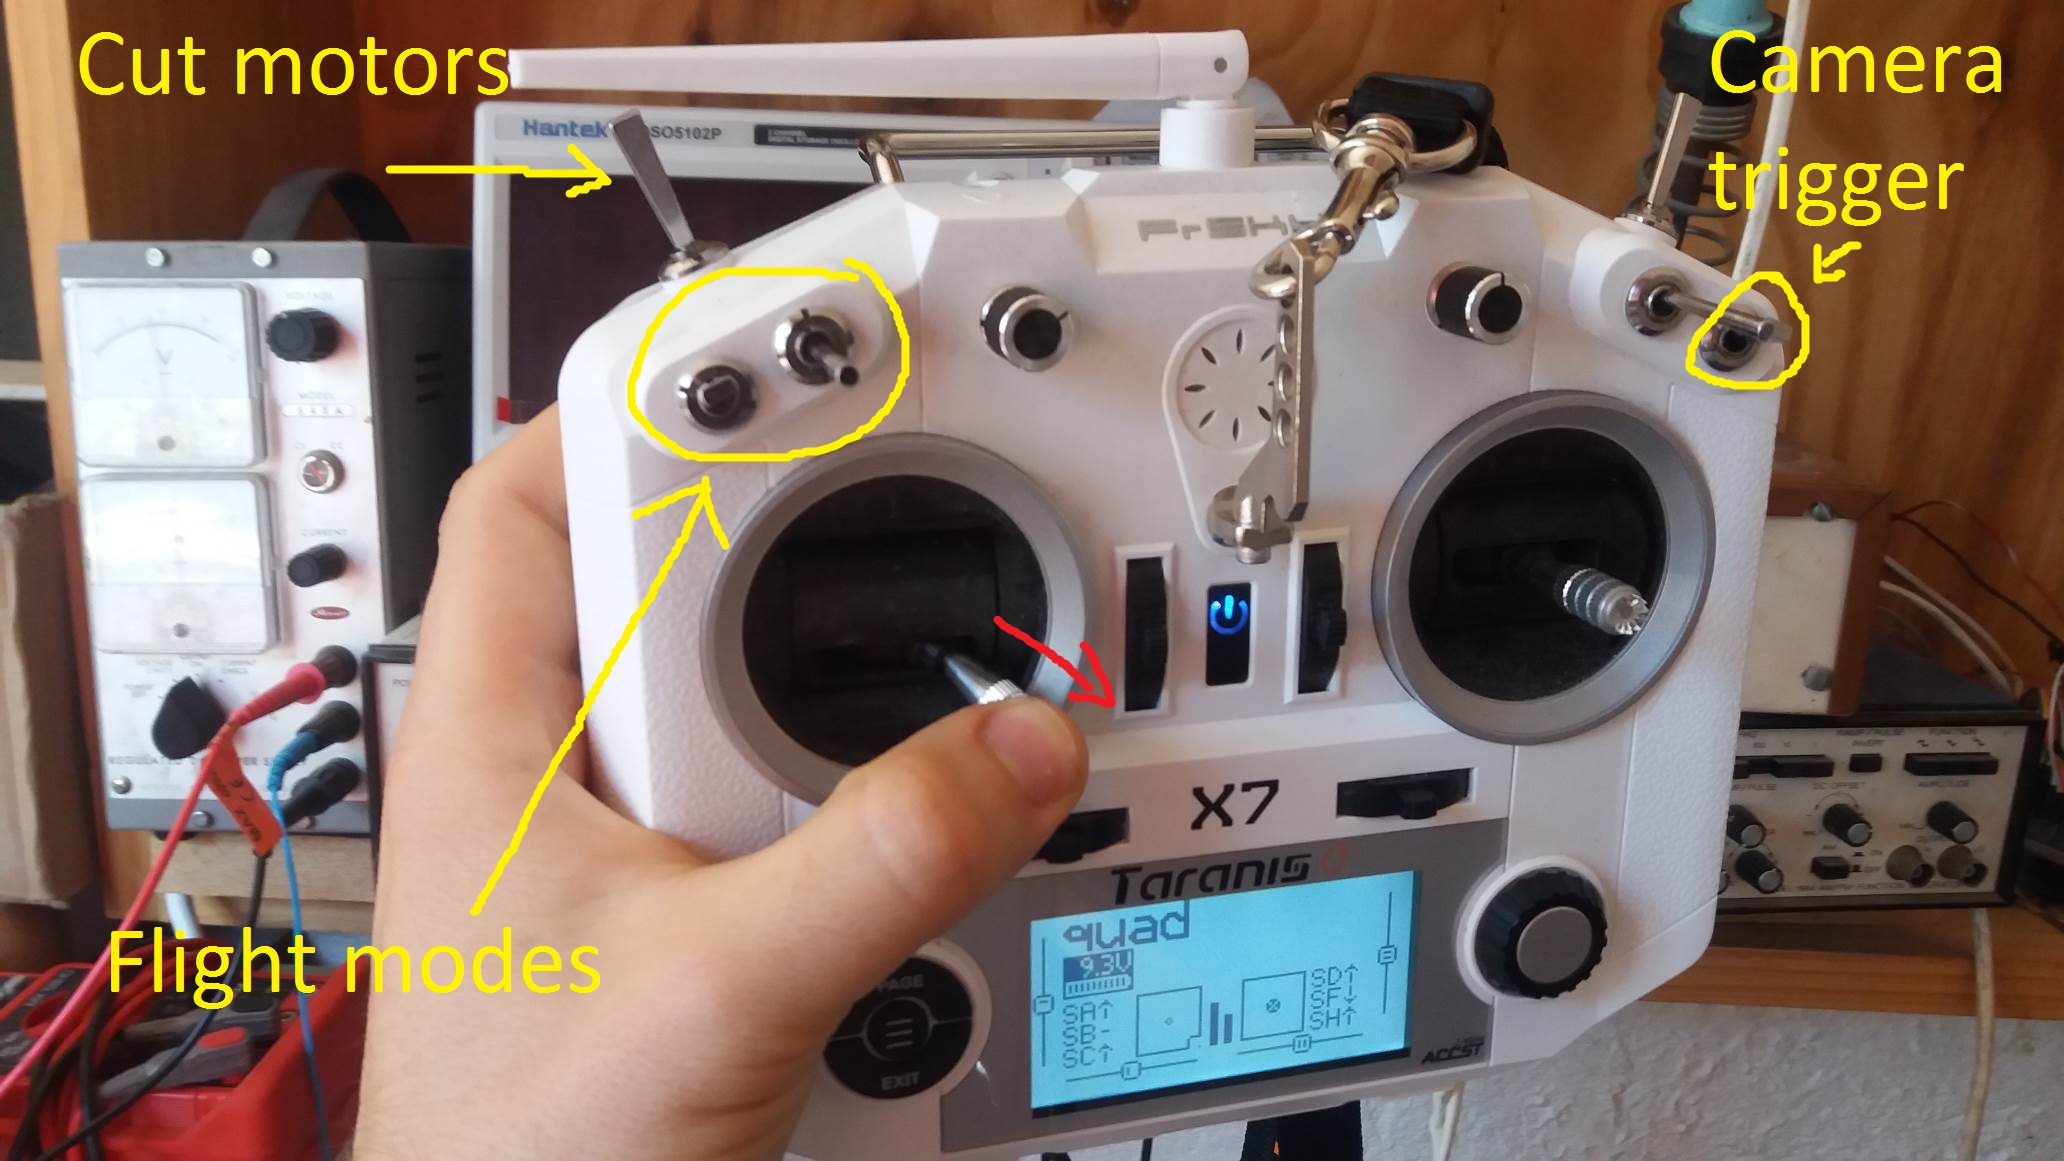
\includegraphics[scale=0.17]{images/taranis_arm.jpg}
\caption{Arming the drone (red arrow)}
\label{fig:taranis_arm}
\end{figure}

\section{Software}

This will be handled by two Raspberry Pis. Both will be used to take photos through each of their single CSI ports. The Raspberry Pis will communicate with each other via direct ethernet connection. Twisted-pair is not necessary since the driver automatically swaps the RX and TX lines.\\

Initially, one Raspberry Pi was to be used with a camera multiplexer as in Section \ref{sec:simultaneous_trig}, but it didn't work, and therefore two raspberry pis were used. Just as well, as the flight controller uses all but 1 GPIO pin.\\

A real-time kernel will be used for the Ardupilot Firmware used on the `flight controller' Raspberry Pi, extended by a Navio2. \\

\section{Testing}

There was a case where one foot holding vibration dampeners broke and induced an unstable asynchronous frequency when rolling in a certain direction as in Figure \ref{fig:leafy}.

\begin{figure}[H]
\centering
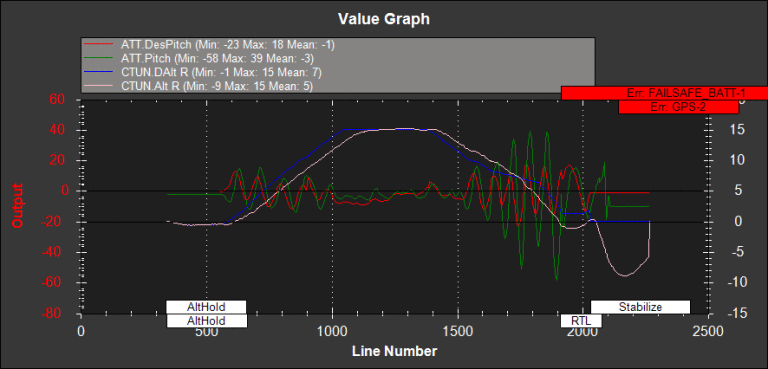
\includegraphics[scale=0.58]{images/pitch_alt.png}
\caption{Oscillations in pitch and roll}
\label{fig:leafy}
\end{figure}

The PID values for pitch and roll rate were lowered by about 11\% to account for the frame size as in Figure \ref{fig:tuning}.\\

\begin{figure}[H]
\centering
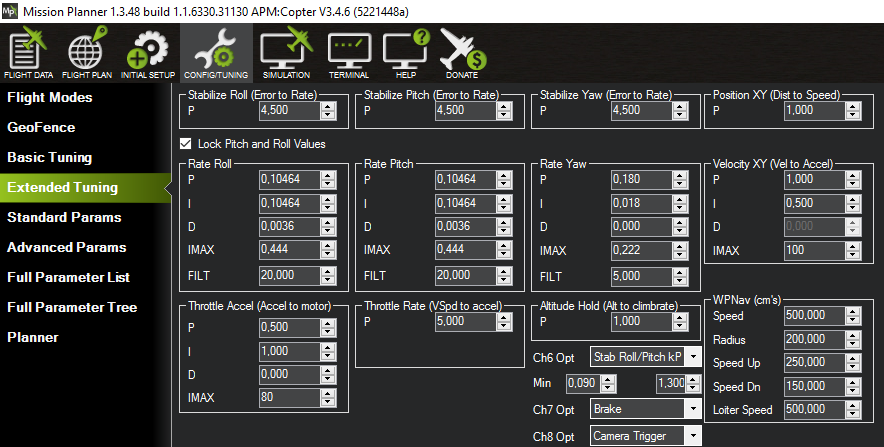
\includegraphics[scale=0.5]{images/tuning.PNG}
\caption{Tuning PID values}
\label{fig:tuning}
\end{figure}

%Relevant flight log data.\\

An RTL2832U software defined radio (SDR) with a receive sensitivity of -140dBm was used to test the range of the 433 MHz transceivers.

\begin{figure}[H]
\begin{subfigure}{0.5\textwidth}
\centering
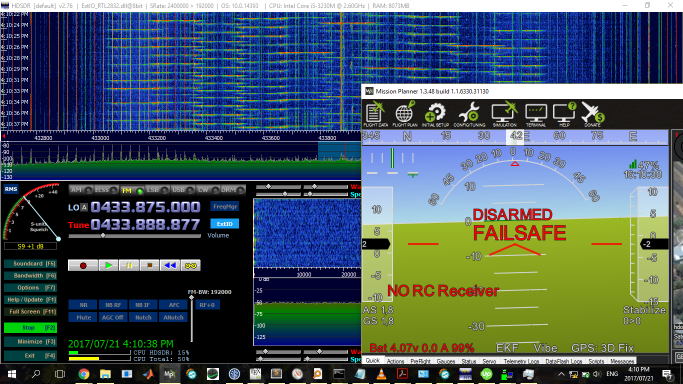
\includegraphics[scale=0.45]{images/range_test.PNG}
\caption{FHSS channel hopping}
\label{fig:range_test}
\end{subfigure}
\begin{subfigure}{0.5\textwidth}
\centering
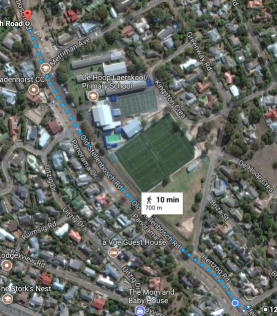
\includegraphics[scale=0.8]{images/range_test_700m.PNG}
\caption{700m NLOS before lost signal}
\label{fig:range_test_700m}
\end{subfigure}
\caption{Range testing}
\label{fig:range}
\end{figure}

Also, compass interference was measured against current draw as in Figure \ref{fig:interference} to lower the chance of errors.

\begin{figure}[H]
\centering
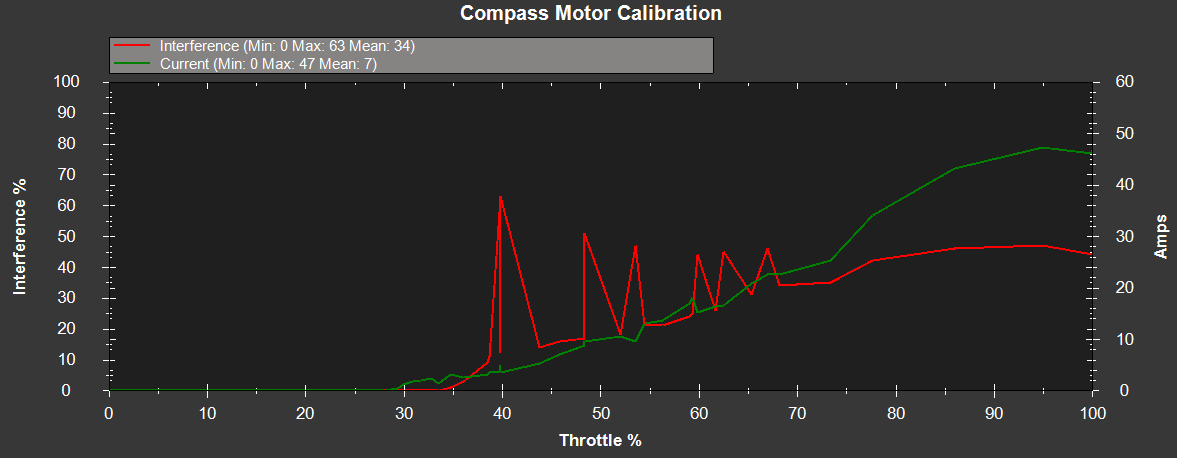
\includegraphics[scale=0.35]{images/comp_mot_true_current.PNG}
\caption{Measuring compass interference vs current draw.}
\label{fig:interference}
\end{figure}


%Many other tests were performed on each component subsystem. For example, a current meter was used to verify the current constants for both power modules, and 